% the following command is only required if the thesis is written in german
%\RequirePackage[ngerman=ngerman-x-latest]{hyphsubst}

% change to english for english theses
\documentclass[english,BCOR=1.5cm,twoside]{tudscrreprt}

\usepackage[T1]{fontenc}
\usepackage[utf8]{inputenc}
\usepackage[english]{babel}
\usepackage{isodate}

\usepackage[
    style=numeric-comp,
    backend=biber,
    url=false,
    doi=false,
    isbn=false,
    hyperref,
]{biblatex}
\addbibresource{bibliography.bib}
\AtEveryBibitem{%
    \clearfield{note}%
}

\usepackage[hidelinks]{hyperref} % makes all links clickable but hides ugly boxes
\usepackage[capitalise,nameinlink,noabbrev]{cleveref} % automatically inserts Fig. X in the text with \cref{..}

\usepackage[colorinlistoftodos,prependcaption,textsize=tiny]{todonotes}

\usepackage{graphicx}
\graphicspath{ {./images/} }

% if you need mathy stuff
\newtheorem{lem}{Lemma}
\crefname{lem}{Lemma}{Lemmas}
\newtheorem{thm}{Theorem}
\crefname{thm}{Theorem}{Theorems}
\newtheorem{defs}{Definition}
\crefname{defs}{Def.}{Defs.}

\usepackage{blindtext}

%\usepackage{tudscrsupervisor} % if you want to copy the sources of the task description into the thesis

\usepackage{csquotes}



\usepackage{caption}
\usepackage{subcaption}
\captionsetup{font=sf,labelfont=bf,labelsep=space}
\usepackage{floatrow}
\floatsetup{font=sf}
\floatsetup[table]{style=plaintop}
\captionsetup{singlelinecheck=off,format=hang,justification=raggedright}
\DeclareCaptionSubType[alph]{figure}
\DeclareCaptionSubType[alph]{table}
\captionsetup[subfloat]{labelformat=brace,list=off}

\usepackage{booktabs}
\usepackage{array}
\usepackage{tabularx}
\usepackage{tabulary}
\usepackage{tabu}
\usepackage{longtable}
\usepackage{xcolor,colortbl}
\usepackage{quoting}

\usepackage[babel]{microtype}

\usepackage{xfrac}

\usepackage{enumitem}
\setlist[itemize]{noitemsep}

\usepackage{ellipsis}
\let\ellipsispunctuation\relax

\usepackage{listings}
\usepackage{inconsolata}

\lstdefinestyle{common-style}{
  basicstyle=\scriptsize\ttfamily,  % the size of the fonts that are used for the code
  showspaces=false,                   % show spaces adding particular underscores
  showstringspaces=false,             % underline spaces within strings
  showtabs=false,                     % show tabs within strings adding particular underscores
%  frame=tlrb,                         % adds a frame around the code
  framexleftmargin=1em,               % space between left part of frame and listing
  tabsize=2,                          % sets default tabsize to 2 spaces
  breaklines=true,                    % sets automatic line breaking
  breakatwhitespace=true,             % sets if automatic breaks should only happen at whitespace
  keywordstyle={\color{blue}\textbf}, % keywords are blue
  commentstyle={\color{gray}},        % comments
  literate={\$}{{{\$}}}1,
  basewidth=0.5em,
  breakindent=40pt,
  breakautoindent=true,
  escapechar=\&,
  aboveskip={0.1\baselineskip}
}

\lstdefinestyle{shortlisting}{
	xleftmargin=\parindent,
	frame=none,
	aboveskip=3pt,belowskip=3pt
}

\lstdefinestyle{unboxed}{
  style=common-style,
	frame=none,
}

% JastAdd
\lstdefinelanguage{AST}{
	style=common-style,
	morekeywords={abstract,rel},
	otherkeywords={::=,->,<,>},
	morecomment=[l]{//}, morecomment=[s]{/*}{*/},
}

\lstdefinelanguage{JRAG}[]{java}{
	style=common-style,
	morekeywords={abstract,public,private,boolean,aspect,null,syn,inh,coll,eq,with,int,contributes,new,return,for,if,else,this,to,true,false},
	morecomment=[l]{//}, morecomment=[s]{/*}{*/},
}

\newcommand{\lstbg}[3][0pt]{{\fboxsep#1\colorbox{#2}{\strut #3}}}
\lstdefinelanguage{diff}[]{java}{
  style=common-style,
  morecomment=[f][\lstbg{HKS07!30}]-,
  morecomment=[f][\lstbg{HKS65!30}]+,
  morecomment=[f][\textit]{@@},
  %morecomment=[f][\textit]{---},
  %morecomment=[f][\textit]{+++},
}

\lstdefinestyle{AST} { language=AST,style=common-style } 
\lstdefinestyle{JRAG} { language=JRAG,style=common-style }
\lstdefinestyle{Java} { language=Java,style=common-style }


\newcommand{\todoD}[1]{\todo[color=green,inline,size=\small]{Dmytro: #1}}
\newcommand{\todoJ}[1]{\todo[color=green,inline,size=\small]{Johannes: #1}}
\newcommand{\todoR}[1]{\todo[color=yellow,inline,size=\small]{Roman: #1}}

\definecolor{Gray}{gray}{0.85}
\newcolumntype{a}{>{\columncolor{Gray}}c}

\begin{document}

\faculty{Faculty of Computer Science}
\department{}
\institute{Institute of Software and Multimedia Technology}
\chair{Chair of Software Technology}
\title{%
    Systematic Parameter Tuning of Genetic Optimization Approaches
}

%% for a bachelor thesis
%\thesis{bachelor}
%\graduation[B.Sc.]{Bachelor of Science}

% for a master thesis
\thesis{master}
\graduation[M.Sc.]{Master of Science}

% for a diploma thesis
%\thesis{diploma}
%\graduation[Dipl.Inf.]{Diplom-Informatiker}

\author{Roman Kosovnenko}
%\emailaddress[]{roman.kosovnenko@mailbox.tu-dresden.de}
\matriculationnumber{4733290}
\matriculationyear{2017}
\dateofbirth{18.1.1994}
\placeofbirth{Chernihiv}
%\discipline{Distributed Systems Engineering}

\course{Distributed Systems Engineering}

\supervisor{%
%	Dipl.-Inf. ABC XYZ%
	M.Sc. Dmytro Pukhkaiev
	\and Dipl.-Inf. Johannes Mey
    \and Dr.-Ing. Sebastian Götz%
}
\professor{Prof. Dr. rer. nat habil. Uwe Aßmann}
\date{9.3.2020}
\maketitle
\newpage

\section*{Acknowledgment}
I would like to take this opportunity to express my immense gratitude to all those who given their invaluable support and assistance.

I wish to express my deepest gratitude to my supervisors M.Sc. Dmytro Pukhkaiev, Dipl.-Inf. Johannes Mey and Dr.-Ing. Sebastian Götz, who convincingly guided and encouraged me to do the right thing even when the road got tough. Without their persistent help, the goal of this thesis would not have been achieved.

I am extremely grateful to my parents for their love,  support, and faith in my decisions.  Also, I express my thanks to my sister for her support. 

Last but not least, I would like to thank my friends and the people around me. They all kept me going. 

\tableofcontents
\listoffigures
\listoftables

\chapter{Introduction}\label{intro}
The optimization problem occurs in all aspects of our life. There exist different methods to solve optimization problems. One of them is the evolutionary computing~(EC) approach. The evolutionary algorithms~(EAs) are part of EC. EAs could solve many optimization problems. It is especially useful when the user does know additional information about the problem. All algorithms of EAs are based on variants of operators and parameters. It means that parameter values could influence the solution of the optimization problem. This thesis describes parameter tuning and parameter analysis of the genetic optimization approach of solving a problem of software variant selection and hardware resource allocation.  

This chapter describes the motivation for parameter tuning and analysis of the genetic optimization approach and marks out research questions to be answered in this thesis. It additionally outlines a solution and contains an overview of the thesis structure.

\section{Motivation}
Researchers and developers know that good parameter values could improve the results of the algorithm. However, searching for optimized parameter values is another problem that needs to be solved. This problem is one of the persisting challenges of the EC field~\cite{smit2010parameter}. The main problem is that the specific EA contains unique design choices presented in the form of operators or its parameters. 

There exist many recommendations about what values are preferable~\cite{de2007parameter, sipper2018investigating}.  But in experimental researches~\cite{de2007parameter, shahookar1990genetic, gockel1997influencing}, these recommendations does not work. 

As a result, parameters need to be tuned. EAs have two approaches for parameter setting: parameter tuning and parameter control. Parameter control could change the parameter value during the EA work. Parameter tuning finds optimized values before EA starts.

According to~\cite{ahmad18}, the genetic optimization approach solves less number of problems than other approaches does. Optimized parameter values could improve the results. This thesis aims to overcome the gap between approaches and improve the genetic optimization approach using parameter tuning.


\section{Objective}
The goal of this thesis is to improve a previously developed genetic optimization approach using parameter tuning.
The research objective is to identify and/or introduce parameters that can improve the genetic optimization approach in terms of its performance and scalability and the quality of the obtained solution. We need to answer the following research questions in order to reach the research objective: 
\begin{itemize}
	\item \textbf{RQ1}: Does the parameter tuning improve the results, and what effect does it give?
	\item \textbf{RQ2}: Were there any bad design choices in the genetic solver? Is there any way to improve it?
\end{itemize}

To answer these questions, we are using several methods that improve the genetic optimization approach. Moreover, we evaluate it on each stage. 

\section{Solution}

The suggested modifications improve the results of the genetic approach and consist of several steps.
The first step is searching for externally changeable parameters. These parameters we are optimizing. 
The second step is exposing parameters for external tuning because most parameters of the genetic solver are not exposed to external change.
Results at this point show that parameter tuning improves the result of the genetic solver, but for further improvement, it requires more modifications.
We introduce fine-grained crossover and mutation points by adding additional probabilities. Parameter tuning so far gives \textbf{valid results}. 

Due to the fact that the number of unique elements goes down on each iteration, we describe two methods to solve this issue.

Simple parameter control that stops the crossover if the part of unique elements in a population is lower than some value. This value is also a parameter. 
The population without duplicates is a second method to save population diversity. This method makes all individuals unique but slows down the solver.

The evaluation shows that fine-grained crossover/mutation points and parameter tuning give the best results for the genetic solver.
The results are improved not only in terms of solution validity but in terms of scalability.


\section{Overview}
This thesis is organized as follows: In Chapter~\ref{chapter:background}, we extend not advanced in the field of software selection and hardware resource allocation problem, evolutionary algorithms, and parameter tuning reader by background knowledge and defines the scope of the thesis. Chapter~\ref{chapter:Implementation} describes an iterative approach to improving the genetic approach. The evaluation results and analysis could be found in Chapter~\ref{chapter:evaluationAnalysis}. Finally, Chapter~\ref{chapter:conclusion} concludes the thesis and Chapter~\ref{chapter:futureWork} describe the future work.

\chapter{Background}
This thesis is based on several kinds of research of auto-tuning, evolutionary algorithms, and software optimization. This chapter summarizes the important aspects and details of approaches and optimization techniques used in the succeeding chapters.  

\section{Multi-Quality Auto-Tuning~(MQuAT)}
Multi-Quality Auto-Tuning (MQuAT) – is an approach to self-adaptive software, which provides design and operation principles for software systems that automatically provide the best possible utility to the user while producing the least possible cost.
It is based on the design-time part, which represents a new development method for self-optimizing systems and runtime parts, which concerns operation principles, namely,  novel techniques to runtime self-optimization~\cite{gotz13}.

\subsection{Design principles of MQuAT}
MQuAT presented a new method of developing self-optimized software. In which software is proposed to be constructed from components with specifically defined limits. In addition, components are intended to comprise multiple implementations, each providing the same but differing functionality in their non-functional behavior. Therefore, the design principle is the critical factor for runtime optimization because when there is a different configuration, optimization can be done, and the optimal or almost optimal configuration can be selected. To compare different implementations of the software component, they need to be specified with their non-functional properties (NFP)~\cite{gotz13}.
A new meta-architecture of the self-optimizing software system was created To highlight this fundamental principle. It called the cool component model~\cite{gotz10}.
A specialty of MQuAT is the application of QoS contracts to cover non-functional implementation behavior as well as the interrelationships of different components between NFPs. Contracts naturally describe the relationship between provisions and requirements.

\subsection{Operation principles of MQuAT}
The core runtime approach proposed in MQuAT is the THE Auto-Tuning Runtime Environment (THEATRE)\cite{gotz10, gotz12}.
The concept of runtime environment contains three layers: a user, software, and a resource layer. All of them depicted in Figure ~\ref{fig:threelayersmquat}
\begin{figure}
	\centering
	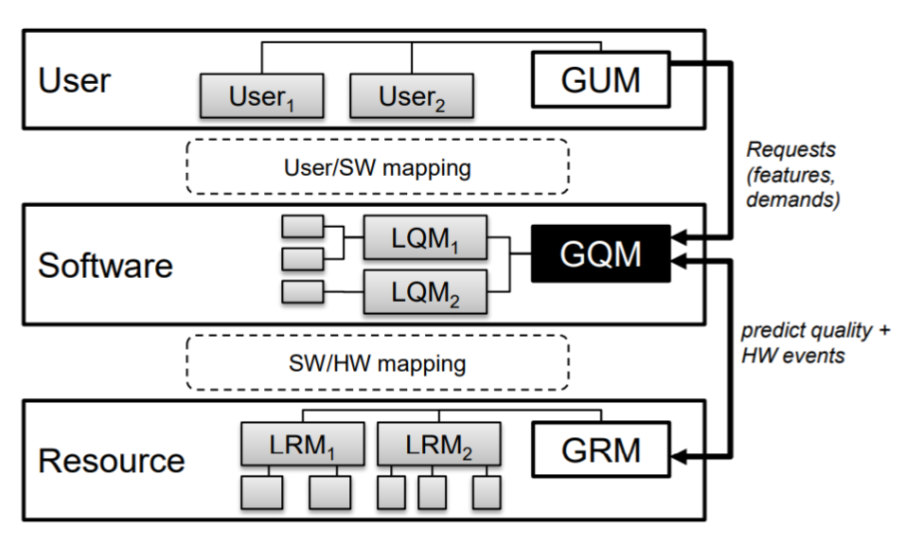
\includegraphics[width=\textwidth]{images/ThreeLayersMQuAT}
	\caption[Three layers of MQuAT]{Three layers of MQuAT}
	\label{fig:threelayersmquat}
\end{figure}

The user layer invokes features and identifies their specifications. The  Global  User  Manager  (GUM)  is required to manage the mapping between users and software component implementations and to coordinate the requests. User requests are minimal software system specifications that have to be met to satisfy the user. The general aim of the runtime system is to help the user as effectively as possible about the purposes of the user~\cite{gotz13}.

The software layer contains all software components, and it's implementations. Each component has a Local Quality Manager(LQM), which responsible for controlling the set of components~\cite{gotz13, ahmad18}. Also, there is a single Global Quality Manager (GQM) which carry out the study and preparation phases of the feedback loop, while the LQM is responsible for the implementation process~\cite{gotz13}.

The resources layer comprises physical (e.g., CPU or RAM) as well as virtual resources(e.g., operating system).
To controlling and monitoring all resources, the Global Resource Manager(GRM) is presented. Each resource has its own Local Resource Manager (LRM), which has in-depth knowledge about its resource and the ability to steer the resource by~\cite{gotz13, ahmad18}.

\subsection{MQuAT combine the design time and runtime}
\begin{figure}
	\centering
	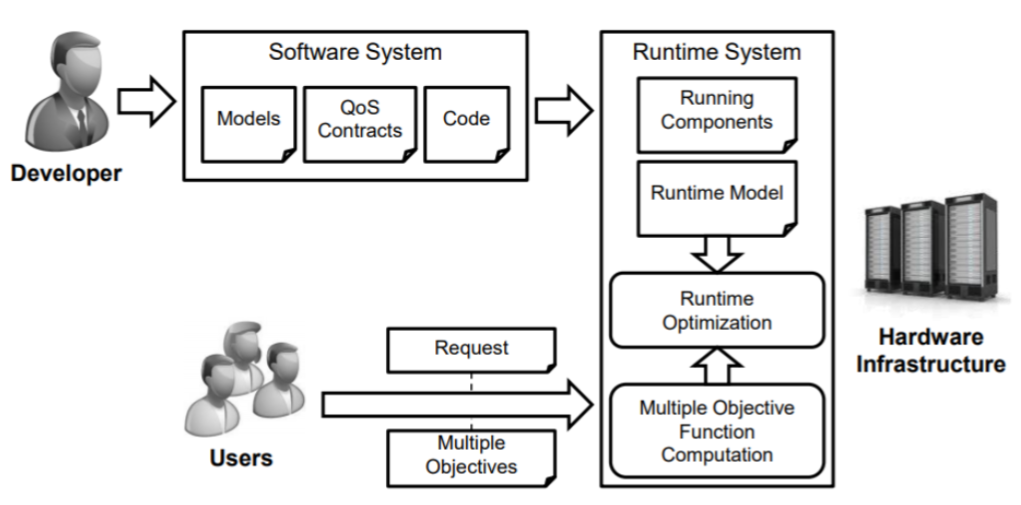
\includegraphics[width=\textwidth]{images/CombinedMQuAT}
	\caption[Combined structure of MQuAT]{Combined structure of MQuAT}
	\label{fig:CombinedMQuAT}
\end{figure}
As showed in Figure ~\ref{fig:CombinedMQuAT}, in addition to the actual code, the developer is creating the models and quality contracts. The users interact with the system at runtime and prepare their objectives and requests. 
In addition to the running components, the runtime system includes a runtime model, representing the current state of the system. The objectives of the user are transformed into objective functions of an optimization program prior to optimization. Depending on the type of optimization technique used, either all users ' objectives are merged into a single objective function, or one objective function is extracted per purpose. Such objective functions and the system's runtime model are used by the runtime optimization method to produce formulations of the optimization problem for the respective technique. Finally, the system determines whether the optimal configuration differs from the actual configuration~\cite{gotz13, ahmad18}.

For more details about MQuAT, please read refer~\cite{gotz13}. For this thesis, we are discussing a solver of the MQuAT problem that is based on MQuAT. Hence, detailed knowledge about MQuAT is not required. 


\section{MQuAT problem}

MQuAT problem was presented in ~\cite{gotz18}, and it consists of two problems:

\begin{itemize}
	\item Resource allocation in which the mapping of software component implementation to hardware resource leads to the least cost
	\item Variant selection, which provides the best utility by selecting better software implementations.
\end{itemize} 

To solve this problem was presented new generic metamodel. Both problems are interrelated by user requests specifying minimum requirements on the provided non-functional properties (i.e., minimum utility) while searching for a selection and mapping both to maximize utility and minimize costs. Correctness denotes that only solutions that \textit{do not violate} the users minimum requirements are considered \textbf{valid}.

The problem to be solved is selecting variants of software components and mapping them based on user requests to suitable hardware resources.

The MQuAT problem could be described as a metamodel which consists of:
\begin{itemize}
	\item Hardware metamodel, which consists of hierarchically structured resource types and resources as instances of these types. So the hardware model composes static awareness of resources (types) and knowledge of runtime (instances). Certain types of resources can run the software, i.e., they are valid targets for software implementation mapping. The container attribute is used to mark such types. Figure~\ref{fig:HWmodel} depicted Hardware metamodel.
	\begin{figure}
		\centering
		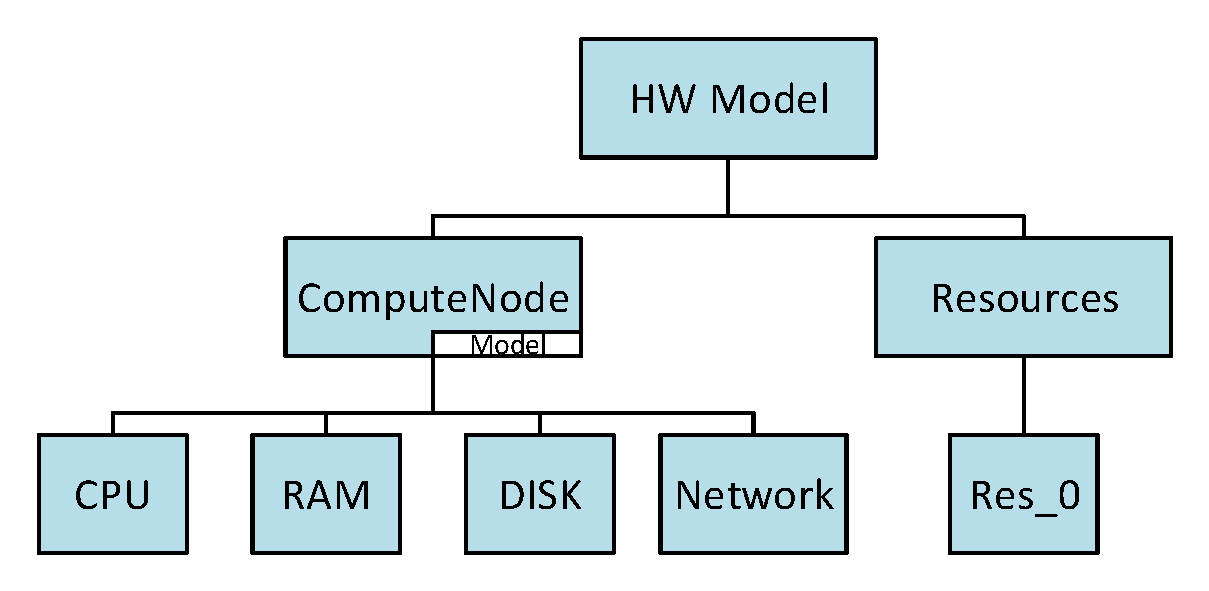
\includegraphics[width=\textwidth]{images/HWModel}
		\caption[Hardware meta-model]{Hardware meta-model}
		\label{fig:HWmodel}
	\end{figure}

	In addition, a set of properties further characterize resource types. Resources specify then specific values for these properties. As an example, the resource type RAM could be defined with a property amount of memory and marked as a container
	\item Software metamodel showed on Figure~\ref{fig:SWModel}. Its main element called component and represents some functionality.
	Each component consists of implementations that provide this functionality, requiring additional components or resources to complete their work. 
	\begin{figure}
		\centering
		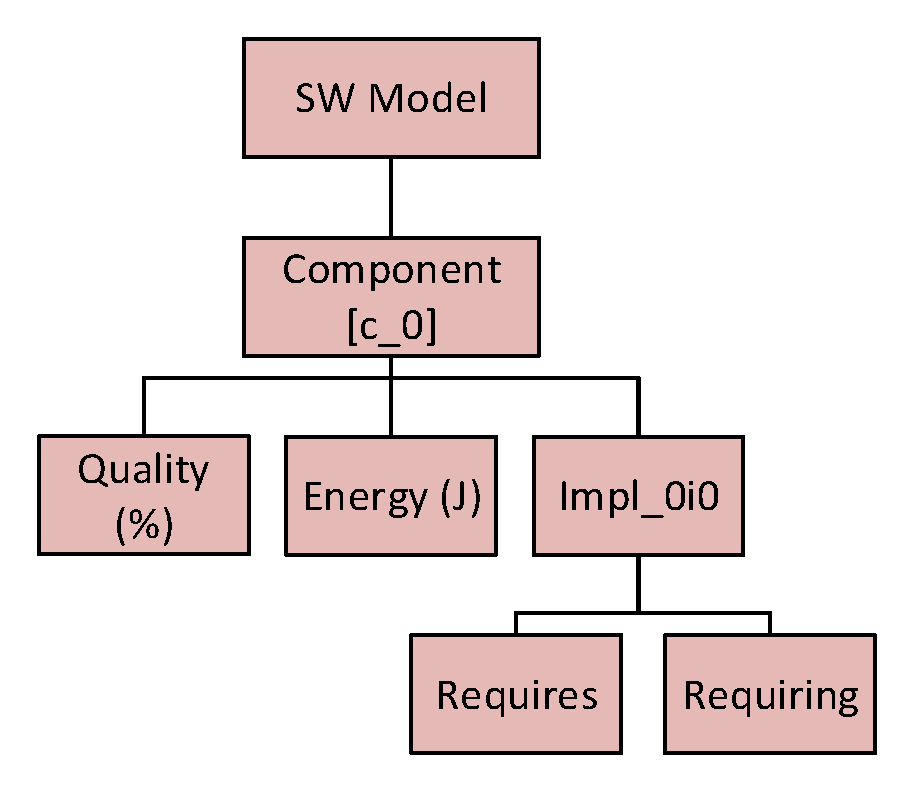
\includegraphics[width=0.75\textwidth]{images/SWModel}
		\caption[Software meta-model]{Software meta-model}
		\label{fig:SWModel}
	\end{figure}
	\item The Objective specifies how to calculate a solution's objective value, i.e., for which value(s) the problem should be optimized. This selects a property to optimize for, and an objective function to define how to aggregate all values of this property.
	\item A Request represents a user requirement, which specifies which algorithm should be used to execute parameters and requirements. Requests contain their functional requirements by referring to a target software component, limitations on non-functional requirements (e.g., quality).
\end{itemize}
Full problem depicted on Figure~\ref{fig:mquatmodel}
\begin{figure}
	\centering
	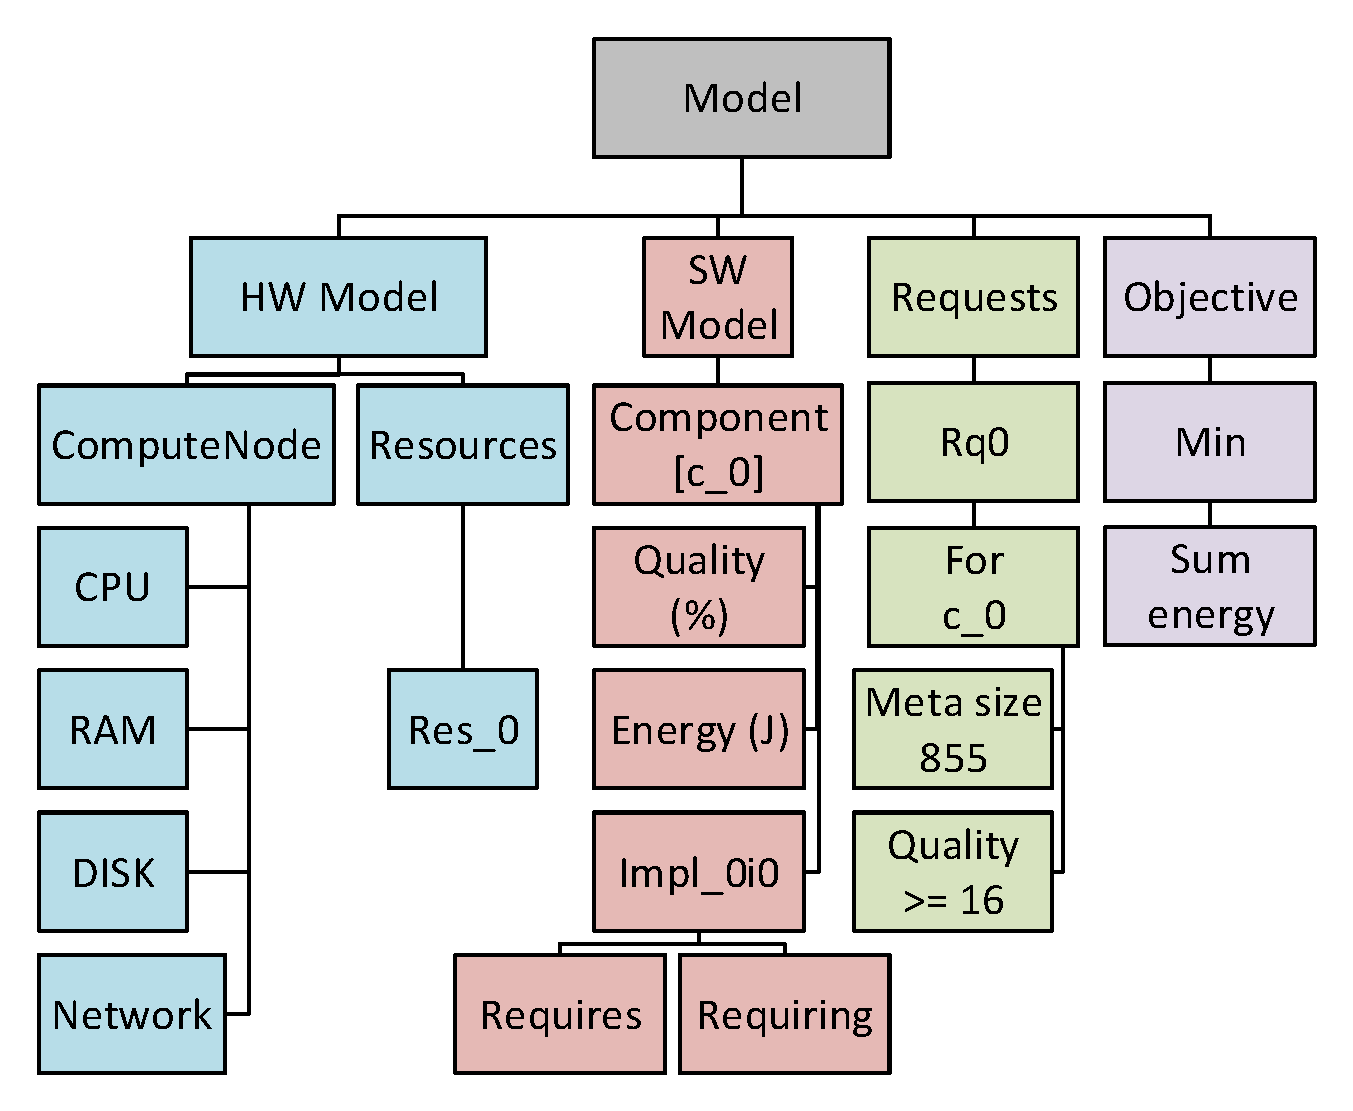
\includegraphics[width=\textwidth]{images/MQuATModel}
	\caption[MQuAT problem model]{MQuAT problem model}
	\label{fig:mquatmodel}
\end{figure}

There are some constraints that are grouped in Architectural, Request, and Negotiation constraints groups.
\begin{itemize}
	\item Architectural constraints ensure that each request is fulfilled, selecting exactly one implementation per component and deploying no more than one implementation on one resource.
	\item Request constraints ensure components are selected for each request so as to provide the requested non-functional properties.
	\item Negotiation constraints ensure non-functional requirements are met depending on the implementation.
\end{itemize}
There are additional constraints due to problem generation:
\begin{itemize}
	\item structures for the software and hardware components are fixed to ensure comparability,
	\item computeNode that represents a regular computer hardware consist of one or more CPUs, RAM memory, disk, and a networking interface,
	\item software model has a simple tree structure,
	\item fixed branching factor of two.
\end{itemize}
Each MQuAT problem is characterize by four parameters:
\paragraph{variants} - the number of implementations for each software component,
\paragraph{requests} - the number of requests to run software components, that described by user, 
\paragraph{depth} - depth of the software tree, that describes dependency of software components,
\paragraph{resources} - resource ratio of the minimally required resources.

\section{The solution of the MQuAT problem}
The solution is computed by the MQuAT solver. There are many solvers:
\begin{itemize}
	\item Simple solver, which goes step by step from one solution candidate to another.
	\item ILP solver, which generates integer linear programming (ILP) problem from the MQUAT problem and after that solve it.
	\item Random solver - tries random solution candidates.
	\item Simulated Annealing (SA) solver, based on the simulated annealing meta-heuristic~{pukhkaiev19}.
	\item Genetic solver that uses a genetic algorithm to solve the problem.
\end{itemize}
In this thesis, we talk about Genetic solver in detail in the next sections.
The solution could be represented as a tree structure. An example of the solution shown in Figure ~\ref{fig:SolutionModel}

It contains a list of assignments. Each assignment select one implementation of required component and map it to the resources~\cite{gotz18}.
A solution is valid if for each user request
\begin{enumerate}
	\item an implementation is deployed for the target component,
	\item for each component required implementation is deployed,
	\item all necessary (non-functional) property clauses (including request constraints) are met,
	\item at most one implementation for each resource is deployed.
\end{enumerate}
If it is valid and no other solution has a better objective value, then a solution is optimal~\cite{gotz18}.

\section{Genetic algorithm}
\label{sec:GeneticAlgorithm}
Evolutionary algorithms are a subset of evolutionary computation and belong to set of modern heuristics-based search method.~\cite{vikhar16}
Appeared as a result of the influence of the biological evolution on computer scientists. This domain contains different types.
There are
\begin{itemize}
	\item Genetic algorithm 
	\item Genetic programming
	\item Evolutionary programming
	\item Evolution strategy
\end{itemize}

\begin{figure}
	\centering
	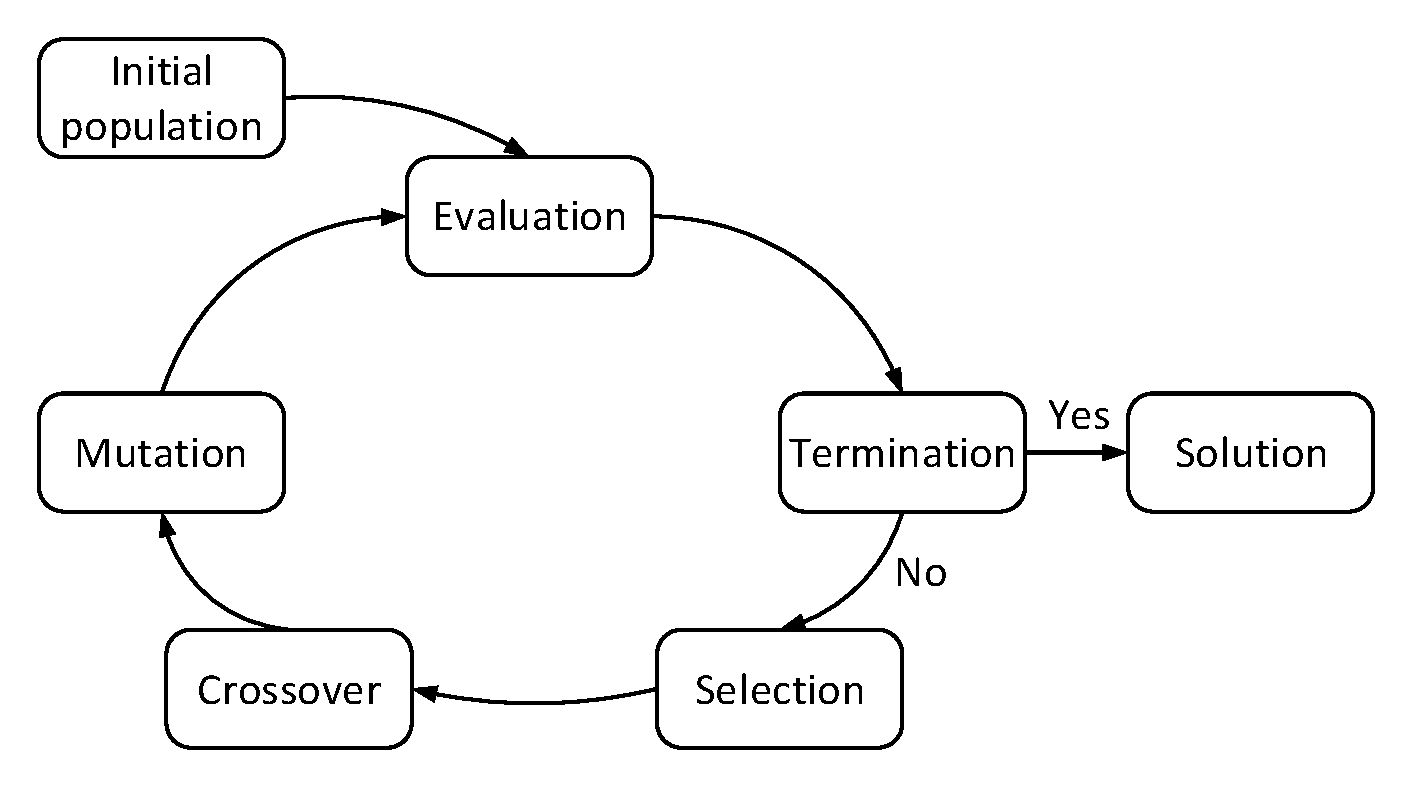
\includegraphics[width=0.8\textwidth]{images/GeneticLoop}
	\caption[Main loop of the genetic algorithm]{Main loop of the genetic algorithm}
	\label{fig:GeneticLoop}
\end{figure}
Main principle of GA looks like a loop with several steps.
The first step is the creation of an initial population - a set of randomly created individuals; each of them represents one solution. 
The second step is Evaluation. Calculate the fitness or objective function of the current population.
If the solution is founded and all requirements for the termination are fulfilled, then we get the final solution. Otherwise, select the best candidates to create a new generation.
In step 4, using recombination and mutation on selected candidates, GA creates a new generation of the population. And after that, evaluate it.

GA based on different components and operators.
\subsection{Selector}\label{sec:GeneticAlgorithm:Selector}
The selector is one of the most important components of GA. It selects \textit{\textbf{mu}} number of individuals from the population, that used to create new \textit{\textbf{lambda}} number of individuals.

There are many different selection algorithms
\begin{itemize}
	\item NSGA2 (Non-dominated sorting based genetic algorithm)
	\item SPEA2 (Strength Pareto Evolutionary Algorithm)
	\item NSGA3\todo{litref}
	\item SPEA3\todo{litref}
	\item PDE \todo{litref}
\end{itemize}
In this thesis, we focus on a selection algorithm only as a parameter of a genetic algorithm and use NSGA2 and SPEA2 due to software constraints of the used framework. 
\todo{Will add more information about selectors}
\subsection{crossover}\label{sec:GeneticAlgorithmCrossover}
Crossover is an operator of a genetic algorithm that allows the recombination of two individuals by swapping some genes between them.
In general, the crossover has several parameters such as
\begin{itemize}
	\item Crossover rate - parameter that describes the probability of two chromosomes to exchange their genes.
	\item Crossover point - the point in which the exchange could be done.
\end{itemize}

The principle of the crossover is next.
Firstly, select the crossover point. For example, a chromosome could be described as a vector of bits. Then the crossover point is the start index of bits, which were replaced by another chromosome.
Secondly, swap genes between chromosomes.

\begin{figure}
	\centering
	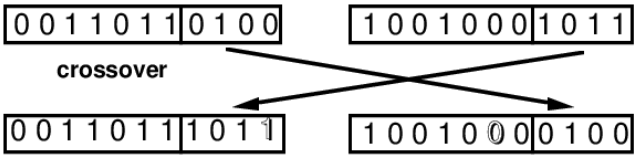
\includegraphics[width=0.5\textwidth]{images/crossoverVector.png}
	\caption[Example of the crossover]{Example of the crossover between chromosome that described as a vector of bits}
	\label{fig:crossoverVector}
\end{figure}

\subsection{mutation}\label{sec:GeneticAlgorithmMutation}

The mutation is an operator of a genetic algorithm that changes a single gene in a chromosome. As a crossover operator, a mutation has parameters:

\begin{itemize}
	\item Mutation rate - parameter that describes the probability of mutation.
\end{itemize}

To perform a mutation on chromosome need to do:
\begin{enumerate}
	\item Randomly select gene which mutates
	\item Change selected gene to another.
\end{enumerate}
\begin{figure}
	\centering
	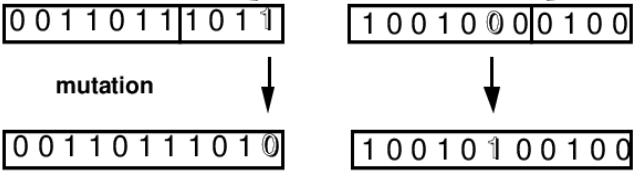
\includegraphics[width=0.5\textwidth]{images/MutationVector.png}
	\caption[Example of the mutation]{Example of the mutation between chromosome that described as a vector of bits}
	\label{fig:MutationVector}
\end{figure}
Figure~\ref{fig:MutationVector} presented a simple mutation on the chromosome that described as a vector of bits.




\section{Genetic solver}
To solve the MQuAT problem using a genetic algorithm, the genetic solver was developed by Jamal Ahmad in ~\cite{ahmad18}. And further improved by Johannes Mey.

This solver is based on Opt4J framework~\footnote{http://opt4j.sourceforge.net/download.html}. It's an open-source framework that gives the opportunity to implement a genetic algorithm for custom optimization problem by specifying several modules and classes.

To solve the custom problem using genetic algorithm, the user needs to create several things:
\begin{enumerate}
	\item Creator is needed to create a random genotype for the initial population.
	In the genetic solver Creator create the genotype by creating a random solution model and transform it into a Tree Shape Genotype structure.
	\item Decoder is needed to perform decoding the tree shape genotype into phenotype. The phenotype, in this case, is a Solution Model of MQuAT.
	\item Evaluator calculates the objective functions of the solution. In the case of genetic solver, the Evaluator calculates two objectives: 
	\begin{itemize}
		\item Validity errors - number of violated contracts
		\item Energy value - energy consumption
	\end{itemize}
\end{enumerate}

If your genotype can't be described as a vector, then you first need to implement:
\begin{enumerate}
	\item Genotype
	\item Crossover operator
	\item Mutation operator
\end{enumerate}

\subsection{Tree Shape Genotype}
Because of the problem model of MQuAT, which requires mapping of implementations to resources, in genetic solver was created Tree Shape Genotype~\cite{ahmad18}.
The example of this genotype shown on Figure~\ref{fig:TreeShapeGenotypeExample}

\begin{figure}
	\centering
	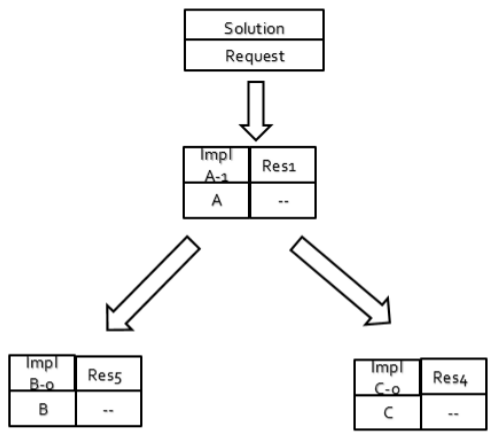
\includegraphics[width=0.6\textwidth]{images/TreeShapeGenotypeExample.png}
	\caption[Example of the Tree Shape Genotype]{Example of the Tree Shape Genotype}
	\label{fig:TreeShapeGenotypeExample}
\end{figure}

The first node in this genotype contains the input request. The second node represents the mapping of the user component. In this node, Impl A-1 is selected rather than Impl A-0 of the user component. As shown in Figure~\ref{fig:TreeShapeGenotypeExample}, this implementation is mapped to Hardware-Resources1. Moreover, Impl A-1 also requires software components B and C that have only one Impl B-0 and Impl C-0 implementation and are mapped to Hardware-Resource5 and Hardware-Resource4, respectively.

\subsection{Crossover operator}
This operator performs a crossover between two Tree Shaped Genotypes and are performed on software implementation and hardware resource in each tree shape genotype. Figure~\ref{fig:GeneticSolverCrossover} depicted the crossover. 
During this process, there is a check that ensures that the implementation and resources are not the same. If this check showed that comparing nodes are the same, then crossover goes recursively to child nodes and performs the check.
If the check showed that nodes are not the same, they swap the implementation, the resource, and all lower substructure.

\begin{figure}
	\centering
	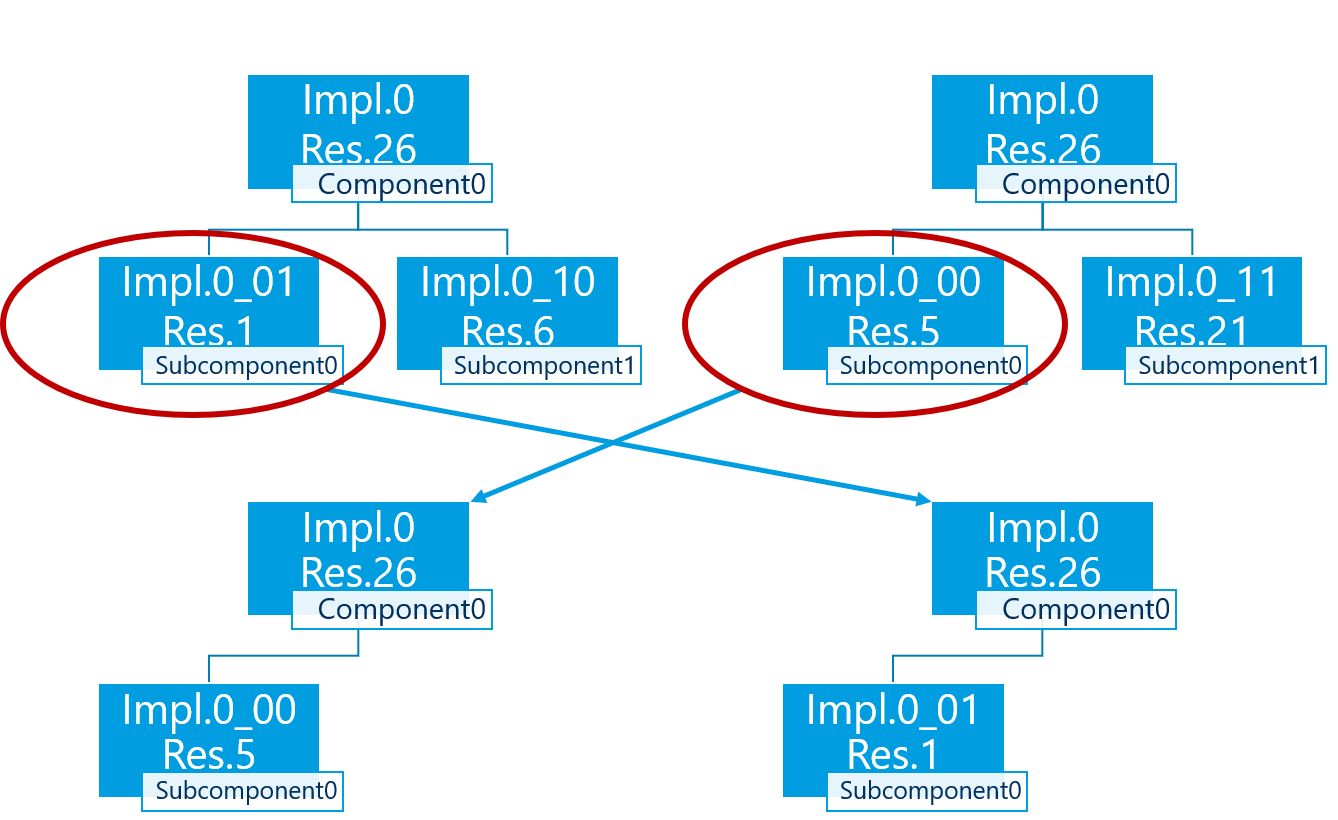
\includegraphics[width=0.9\textwidth]{images/GeneticSolverCrossover.png}
	\caption[Crossover in Tree Shape Genotype]{Example of crossover between two Tree Shape Genotypes}
	\label{fig:GeneticSolverCrossover}
\end{figure}



\subsection{Mutation operator}
Mutation operation is used to randomly add new features to the tree-shaped genotype. Figure~\ref{fig:GeneticSolverCrossover} depicts the mutation process in which with some probability to mutate current node or recursively go down to children.
There are two more probabilities that represent a chance of mutation in implementation and resource accordingly. 

\begin{figure}
	\centering
	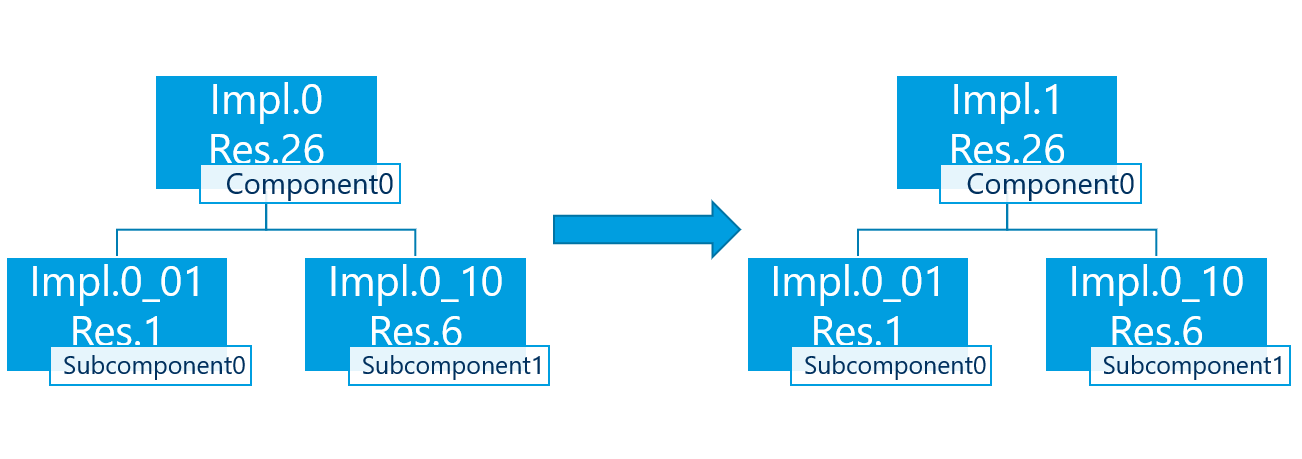
\includegraphics[width=\textwidth]{images/GeneticSolverMutation.png}
	\caption[Mutation in Tree Shape Genotype]{Example of mutation between two Tree Shape Genotypes}
	\label{fig:GeneticSolverMutation}
\end{figure}

\section{Parameter Tuning Strategies for GA}
information from literature!\todo{will add more in next draft}

\section{BRISE}
BRISE is a software product line (SPL) for parameter tuning~\cite{pukhkaiev19}.
This SPL has two conceptual parts:
\begin{itemize}
	\item Static part describes the main flow of parameter tuning, task management, and reporting.
	\item Configurable part should be configured for each experiment.
\end{itemize}

\begin{figure}
	\centering
	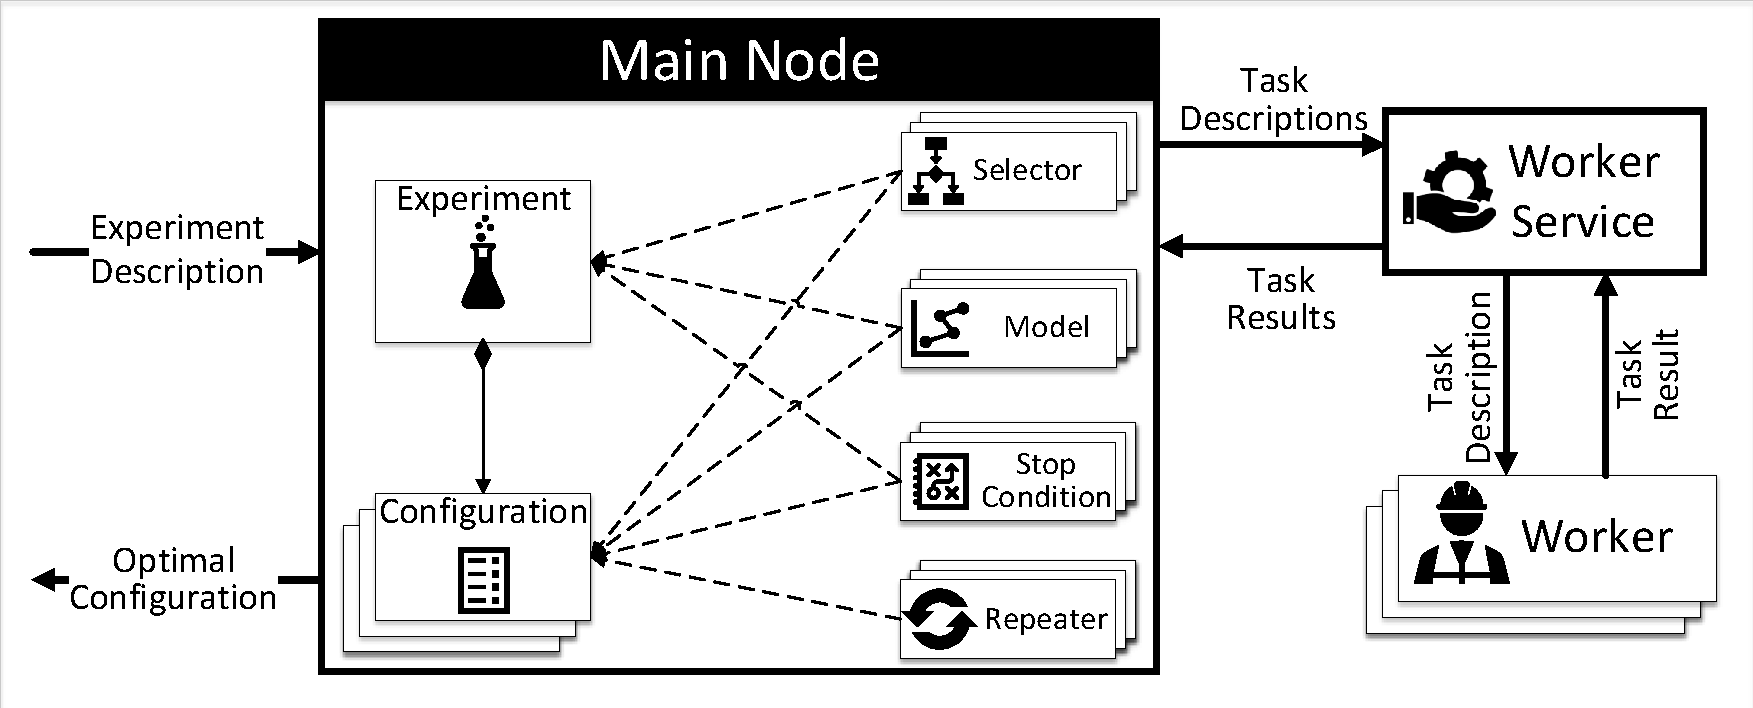
\includegraphics[width=\textwidth]{images/BRISEarch.pdf}
	\caption[The high-level architecture of BRISE]{The high-level architecture of BRISE}
	\label{fig:BRISEarch}
\end{figure}

Figure~\ref{fig:BRISEarch} shown the high-level architecture of BRISE.
Configurable part consist of 
	\paragraph{Experiment description} - describes the experiment, parameters that need to tune, the objective of the experiment, and expected values to detect outliers.
	\paragraph{Selector} - selection algorithm that is used to get the combination of parameters from the search space of all possible combinations. BRISE has two selection algorithms out of the box: Sobol sampling~\cite{sobol99} and Fedorov's exchange algorithm~\cite{fedorov13}. 
	\paragraph{Model} - predict new configuration. New Model builds after each iteration of measurement of configuration, and if Model predicts a valid result, this configuration goes to be measured in the next iteration. BRISE has several models out of the box.
	\paragraph{Stop condition} - the component that analyzes the results of the experiment, validates the result, and makes a decision to stop the experiment or continue. There are many different stop conditions that could work as a combination of criteria.
	\paragraph{Repeater} - component of BRISE that decide about the number of measurement for each configuration to get need accuracy of the results. 
	\paragraph{Worker} - contains the process that BRISE needs to tune. Run this process with different configurations and returns the metric of this configuration to use it in the next model build.
All components from the configurable part could be extended by users to achieve their goals.

BRISE has two modes: \textit{Search space exploration} and \textit{Hyperparameter tuning}.
First one is used to get information about search space of hyperparameters. In this mode there is no predictions cause BRISE uses the selector to cover the search space. As a result of using BRISE without predictions, the model component is disabled. Also stop condition is disabled in this mode and BRISE stops after it have covered all search space. Repeater works as it should to achieve needed accuracy.

The second mode is used to find the optimized values for hyperparameters. All components of the main node are used in this mode.

The main principle of how BRISE works in both modes is the same, but 
Search space exploration mode has one exception.

User prepare metric function that will runing in workers and measure the result for specified configuration of hyperparameters.
After that user describe the experiment description - JSON file that contains all information about hyperparameters, their ranges and default values, result structure, expected ranges for result values and the max time needed to run one task.

The user input of BRISE is experiment description, that in BRISE transforms into Experiment object. After that BRISE start working.

It start with measurement of default configuration. When the default configuration had been measured, selector gives set of new configurations to be measured. After measurments workers return the results to main node. The repeater checks the result and decide to measure this configuration one more time or results has needed accuracy. 

On the next step model component tries to build the model and validate itself. If built model is valid then it predicts new configuration. if the model is not valid, BRISE get new configuration from the selector. BRISE send it to worker service to measure and get the result. If SPL working in Search space exploration mode, the model build step is skipped and new configuration always received from the selector. 

This measurements are performing until stop condition criteria in stop condition component are met.










\chapter{Implementation}\label{chapter:Implementation}

In this chapter we describe several approaches to improve the Genetic Solver by parameter tuning.
We will concentrate on solving the problem with \textbf{5 minutes} timeout and the following properties:
\begin{itemize}
	\item \textbf{Software variants: 10;}
	\item \textbf{Number of requests: 15;}
	\item \textbf{Component tree depth: 2;}
	\item \textbf{Resources ratio: 5;}
\end{itemize}
on the an Intel Core i7-8700 CPU machine with 64Gb of memory using Fedora Server 29 and OpenJDK 1.8.0 201-b09 for \textbf{5 times}.

Our goal is to achieve valid results in terms of contract violations, and then get an optimal or near-optimal solution in terms of energy consumption. 

We mark base~\footnote{As a base version taked version at the master branch from 24.09.2019, commit: \href{https://git-st.inf.tu-dresden.de/mquat/mquat2/commit/57845c126c30a1ea59cb35eb16af0bd37930dda9}{57845c126c30a1ea59cb35eb16af0bd37930dda9}} version of the genetic solver as \textbf{B} (Base).


\begin{figure}
	\centering
	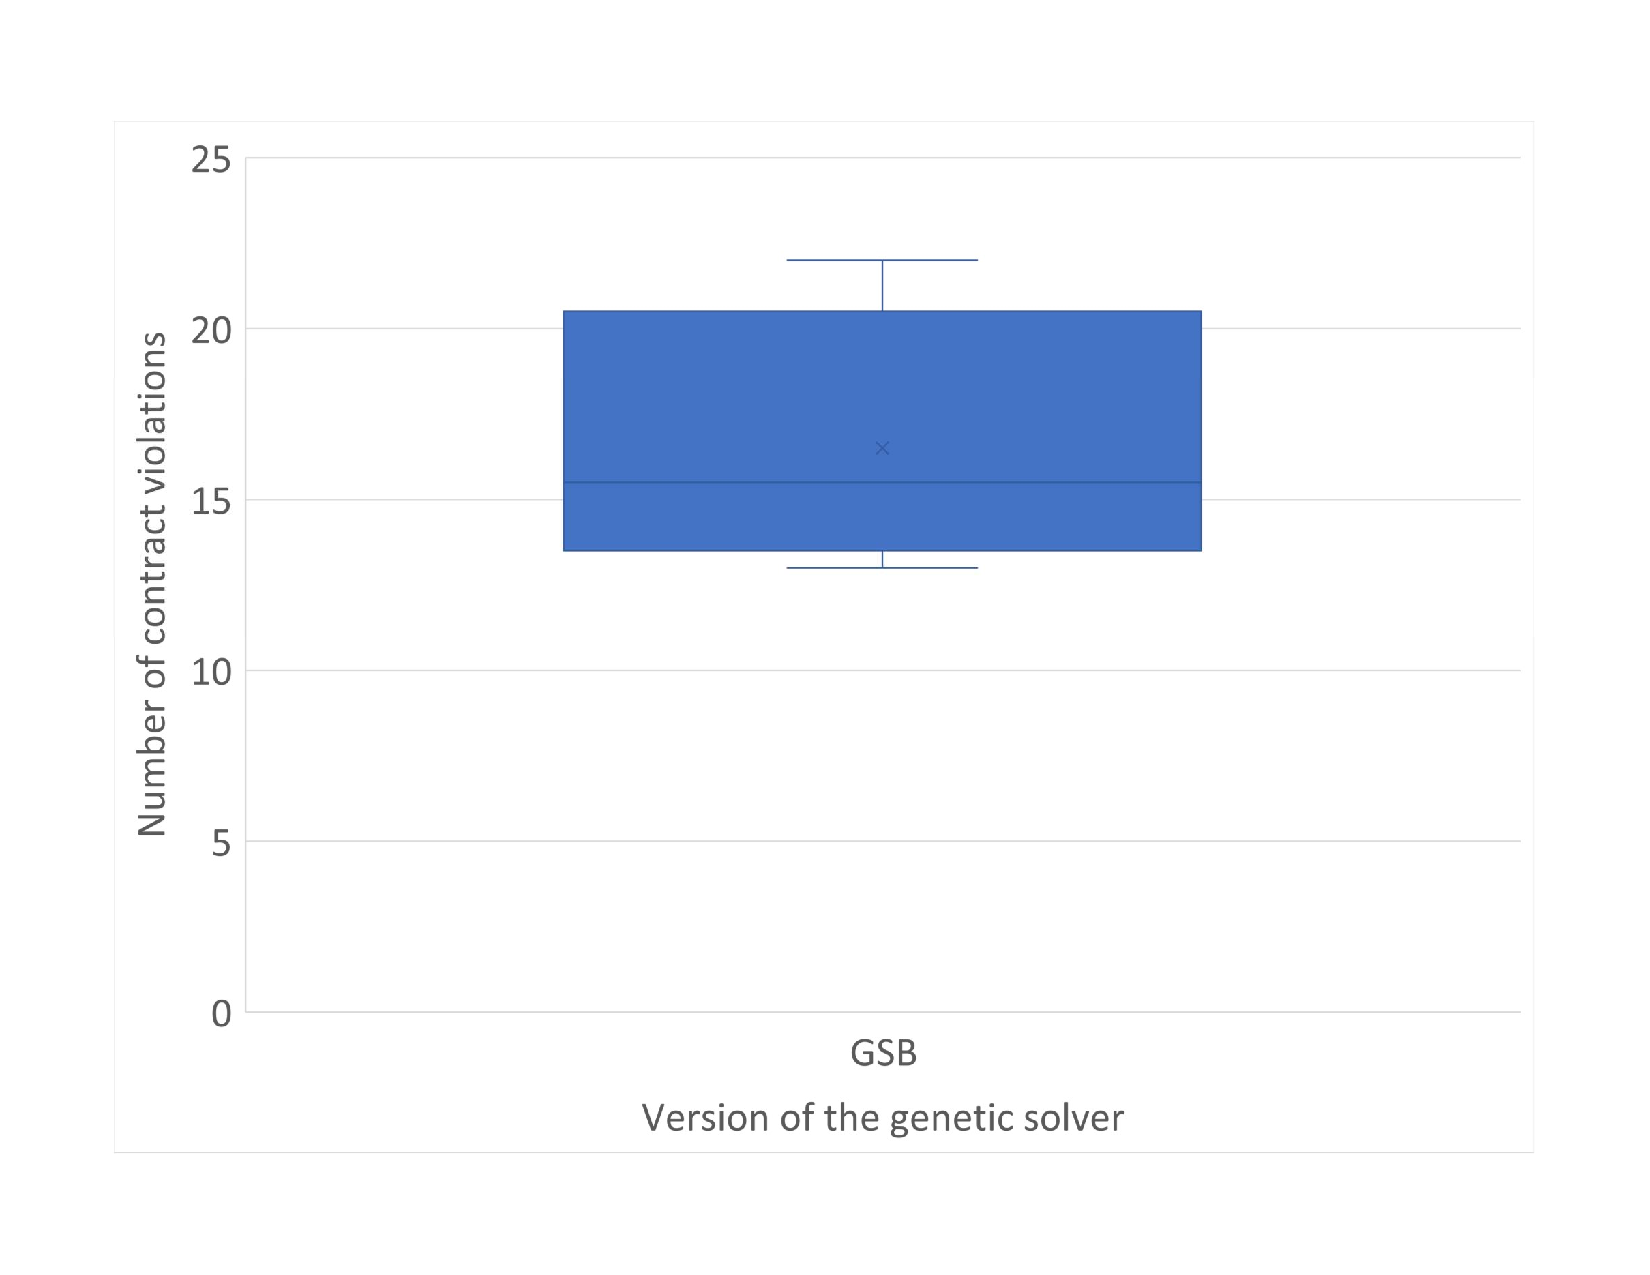
\includegraphics[width=\textwidth]{images/BoxPlotSolverBasic}
	\caption[Boxplot of contract violations for the base version of genetic solver]{Boxplot of contract violations for the base version of genetic solver}
	\label{fig:boxplotsolverbasic}
\end{figure}


Figure~\ref{fig:boxplotsolverbasic} shown the boxplot of the number of contract violations in the base~(\textbf{B}) version of the Genetic Solver. This plot shows that  the base~(\textbf{B}) version solves this task with the number of contract violations in a range from 13 to 22. As a result, there are no valid solutions for the current problem.




\section{First parameter tuning}

The first step to improve the genetic solver was a parameter tuning. To get a set of optimized parameter values it is needed to perform a few essential steps:

\begin{enumerate}
	\item Analyze the genetic solver to find all parameters that could be changed externally. They will be hyperparameters that BRISE will tune.
	\item Adapt BRISE to work with the genetic solver.
	\item Prepare Experiment description for BRISE.
	\item Run BRISE to get the near-optimal configuration of the Genetic Solver.
\end{enumerate}

\textbf{Step 1} involves the analysis of the solver for the presence of parameters that can be changed externally. After diving into the code of the genetic solver, the list of parameters was prepared. Each parameter has a name, short name that consist of capital \textbf{R} and the order number of parameters, the default value that was used in the genetic solver and a range of values for continues parameters or list of values for categorical parameters. The possible value we show with square brackets near the short name. There are:
\paragraph{\texttt{SelectorType}~(R1)~[NSGA2, SPEA2]} - type of the selector algorithm, mentioned in section~\ref{sec:GeneticAlgorithm:Selector}. Default value is \textit{NSGAII};
\paragraph{\texttt{Generations}~(R2)} - number of generations, performed by the genetic solver, working as a termination condition. In this thesis we use only timeout termination. Let us set this parameter in a way, that it does not influence the termination (since the timeout-based termination is used instead);
\paragraph{\texttt{PopulationSize}~(R3)~[100-5000]} - The parameter, that describes the number of individuals in a population. Default value is \textbf{500}. \\

Adaptation of the genetic solver to work in BRISE (\textbf{Step 2}) consists of preparing the executable file of the genetic solver and implementing a method for the worker, which encapsulates execution of the Genetic Solver with specified parameters and returns the results with a number of contract violations and energy consumption.

\textbf{Step 3} means that a user describes hyperparameters that need to be optimized and BRISE components configuration such as selector, repeater, model, and stop condition, list of hyperparameters described by a name, a range of values, or a set of values, the default value.

For parameter tuning of the genetic solver, we use Sobol sampling as a selector algorithm to get the new configuration of hyperparameters, student repeater with a minimal number of measurements - 3 and max number - 6. BRISE uses Bayesian Optimization~(BO) as a prediction model.
To stop BRISE, we use a combination of time-based stop condition with timeout - 12 hours and guaranteed stop condition, which ensures achieving the better result in comparison with the default set of parameters. The experiment description file is presented in appendix\todoR{ref to the appendix with experiment description}.

We use parameter values of the base~(\textbf{B}) version of the Genetic Solver as a default configuration for BRISE. Such decision makes it possible to use a guarantee stop condition. The default parameter values are presented in Table~\ref{tab:Parameters_B-T}. Also, there are a few parameters in gray-colored filling that have a hard-coded value, but we will discuss them in the next section. 

We mark current version~\footnote{commit: \href{https://git-st.inf.tu-dresden.de/mquat/mquat2/commit/e103f52b3333900d61c6218a1f2ca811bca10289}{e103f52b3333900d61c6218a1f2ca811bca10289}} of the genetic solver as \textbf{B-T}(Base-Tuned).


\begin{table}
	\centering
	\caption{Parameters of B and B-T versions of the Genetic Solver}\label{tab:Parameters_B-T}
	\resizebox{\textwidth}{!}{
		\begin{tabular}{c c c a a a a a a a a a a}
			\hline
			\rotatebox{0}{Genetic Solver} & \rotatebox{0}{\texttt{R1}} & \rotatebox{0}{\texttt{R3}} & \rotatebox{0}{\texttt{R4}} & \rotatebox{0}{\texttt{R5}} & \rotatebox{0}{\texttt{R6}} & \rotatebox{0}{\texttt{R7}} & \rotatebox{0}{\texttt{R8}}  & \rotatebox{0}{\texttt{R9}}  & \rotatebox{0}{\texttt{R10}} & \rotatebox{0}{\texttt{R11}} & \rotatebox{0}{\texttt{R12}} & \rotatebox{0}{\texttt{R13}} \\
			\hline            
			B & NSGA2 & 500 & 0.1 & 0.95 & 0.1 & 0.45 & 0.5 & 0.8 & 0.5 & 0.5 & 50 & 100 \\
			B-T & NSGA2 & 1533 & 0.1 & 0.95 & 0.1 & 0.45 & 0.5 & 0.8 & 0.5 & 0.5 & 50 & 100 \\
			\hline
		\end{tabular}
	}
\end{table}

\begin{figure}
	\centering
	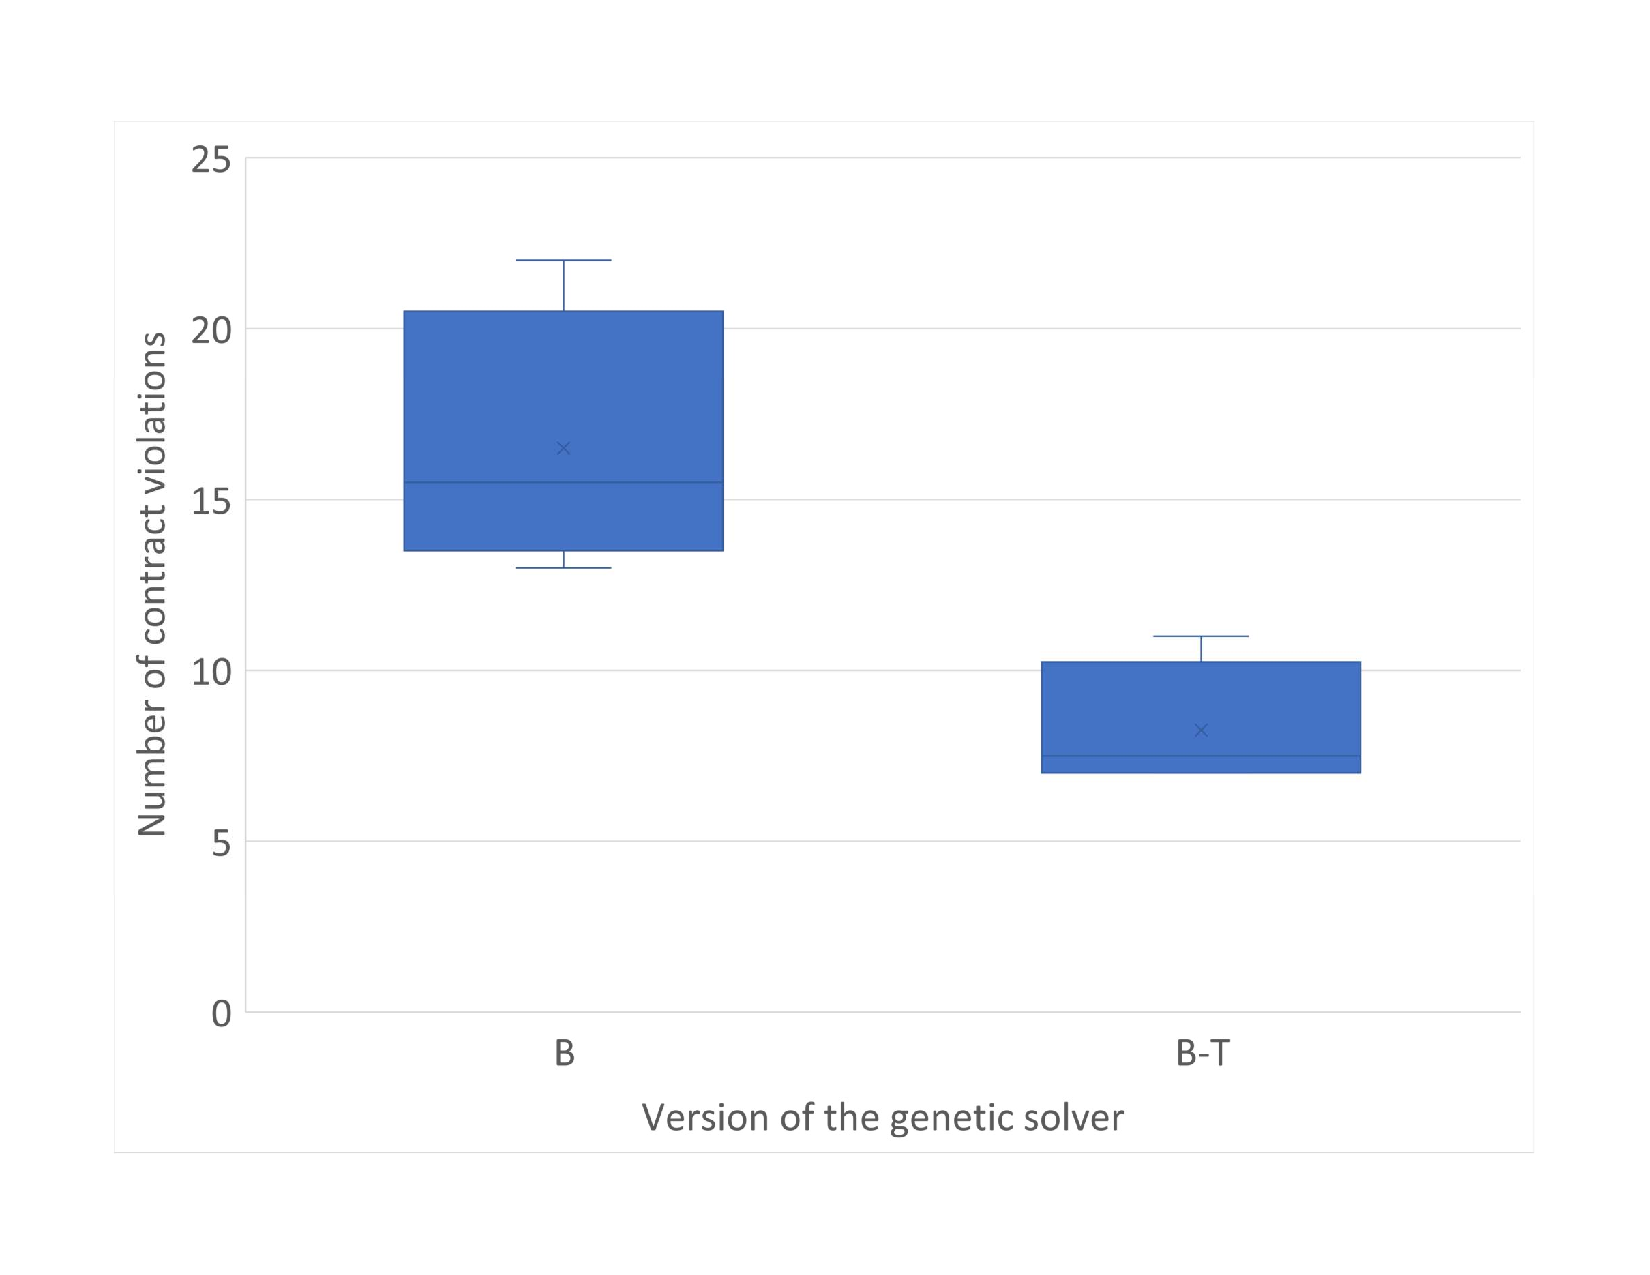
\includegraphics[width=\textwidth]{images/BoxPlotSolverBasicTuning}
	\caption[Boxplot with a number of contract violations for the base version of the Genetic Solver with tuned parameters]{Boxplot with a number of contract violations for the base version of the Genetic Solver with tuned parameters}
	\label{fig:boxplotsolverbasictuning}
\end{figure}

The result of hyperparameter optimization is presented in the Table~\ref{tab:Parameters_B-T}. As showed, BRISE gives a set of parameters with a bigger number of population size~(R3).

The results of solving the earlier described problem as a boxplot showed in Figure~\ref{fig:boxplotsolverbasictuning}. In the Figure~\ref{fig:boxplotsolverbasictuning} also showed a comparison between the base~(\textbf{B}) and its tuned~(\textbf{B-T}) version of the genetic solver. The \textbf{B-T} version of the genetic solver gives a better result compared with the \textbf{B} version. The minimal number of contract violations in the \textbf{B-T} version is almost 2 times fewer than in B version. 

Received results answer the \textbf{RQ1}. Parameter tuning improves results, and it has a positive effect on the genetic solver, but results are still not valid. 

\section{More parameters}

In the previous section, we showed that not all parameters of the genetic solver exposed for tuning. To make them changeable externally, we use \texttt{GoogleGuiceDependencyInjection}\footnote{\url{https://github.com/google/guice}} tool to change the values of these parameters during the solver call. Let us discuss these parameters:
\paragraph{\texttt{lambda}~(R4)~[0.0-1.0]} - as mentioned in Section~\ref{sec:GeneticAlgorithm:Selector}, it is the number of new offspring per generation. We use this parameter as a part of the population size. The default value is 0.1.
\paragraph{\texttt{CrossoverRate}~(R5)~[0.0-1.0]} - as mentioned in section~\ref{sec:GeneticAlgorithmCrossover}, it describes the probability of two individuals to gene exchange. The default value is 0.95.
\paragraph{\texttt{mu}~(R6)~[0.0-1.0]} - as mentioned in section~\ref{sec:GeneticAlgorithm:Selector}, it describes the number of parents, selected by the selector to create new individuals. We use this parameter as a part of the population size. The default value is 0.1.
\paragraph{\texttt{MutationRate}~(R7)~[0.0-1.0]} - as mentioned in section~\ref{sec:GeneticAlgorithmMutation}, it describes the probability of the individual to mutate. BRISE will tune this parameter with default value 0.45 from the base~(\textbf{B}) version of the genetic solver.
\paragraph{\texttt{ResourceMutationProbability}~(R8)~[0.0-1.0]} - the likelihood that during the mutation, the assigned resource will mutate. BRISE will tune this parameter with default value 0.5 from the B version of the genetic solver.
\paragraph{\texttt{CrossoverProbability}~(R9)~[0.0-1.0]} - it describes the probability of doing crossover that checks in the crossover operator. The default value of this parameter is 0.8. This parameter was removed in later versions of the genetic solver because it duplicates the functionality of \texttt{CrossoverRate}~(R5). This fact answers \textbf{RQ2}. It is one bad design choice that we want to find, according to \textbf{RQ2}.\\ 


Within the genetic solver evaluator, two factors penalize the quality of the solution in the case of a contract breach or errors in dependencies in the software tree. These coefficients were not set for external tuning. The default value for all parameters is 0.5.
\paragraph{\texttt{ValidityWeight}~(R10)~[0.0-1.0]} - coefficient that shows how each contract violation decreases the quality of the solution.
\paragraph{\texttt{SoftwareValidityWeight}~(R11)~[0.0-1.0]} - coefficient that shows how each error in the software tree decrease the quality of the solution.\\

As described in Section~\ref{sec:GeneticSolver}, a creator creates random individuals for the initial population.
This method has two features that are necessary to obtain better individuals at the initial stage. These features have parameters:
\paragraph{\texttt{RandomSoftwareAssignmentAttempts}~(R12)~[1-1000]} - max number of attempts to set a valid software tree to the individual on the creation phase. The default value is 50.
\paragraph{\texttt{populateSoftwareSolutionAttempts}~(R13)~[1-1000]} -  max number of attempts to assign software components and resources to get a valid individual on the creation phase. The default value is 100.\\

We mark this version~\footnote{commit: \href{https://git-st.inf.tu-dresden.de/mquat/mquat2/commit/e1db4a941622f9a6609ffcfb5d05df9e7abaffc2}{e1db4a941622f9a6609ffcfb5d05df9e7abaffc2}} of the genetic solver as \textbf{WHC-T}(Without Hard-Code-Tuned).

After optimization, we use an optimized set of values of hyperparameters from BRISE, showed in Table~\ref{tab:Parameters_NHC-T}, as parameters for the \textbf{WHC-T} version genetic solver. As shown with more parameters, BRISE suggests using the \textit{SPEA2} selector algorithm, but the value of the \texttt{CrossoverRate}~(R5) is not changed.

\begin{table}
	\centering
	\caption{Parameters of WHC-T version of the genetic solver}\label{tab:Parameters_NHC-T}
	\resizebox{\textwidth}{!}{
		\begin{tabular}{c c c c c c c c c c c c c}
			\hline
			\rotatebox{0}{Genetic solver} & \rotatebox{0}{\texttt{R1}} & \rotatebox{0}{\texttt{R3}} & \rotatebox{0}{\texttt{R4}} & \rotatebox{0}{\texttt{R5}} & \rotatebox{0}{\texttt{R6}} & \rotatebox{0}{\texttt{R7}} & \rotatebox{0}{\texttt{R8}}  & \rotatebox{0}{\texttt{R9}}  & \rotatebox{0}{\texttt{R10}} & \rotatebox{0}{\texttt{R11}} & \rotatebox{0}{\texttt{R12}} & \rotatebox{0}{\texttt{R13}} \\
			\hline            
			WHC-T & SPEA2 & 2014 & 0.98 & 0.95 & 0.58 & 0.02 & 0.64 & 0.3 & 0.95 & 0.17 & 79 & 266 \\
			\hline
		\end{tabular}
	}
\end{table}

Results of the WHC-T version of the genetic solver presented as boxplot in comparison with earlier versions~(\textbf{B}, \textbf{B-T}) is shown in Figure~\ref{fig:boxplotsolverNoHardcodedTuning}. This boxplot shows that the WHC-T version of the genetic solver is better in comparison to B-T. The max number of contract violations in WHC-T is \textbf{7}. This number is equal to a minimum number of contract violations from the B-T version. But solutions are still \textbf{not valid} for the current problem. 

\begin{figure}
	\centering
	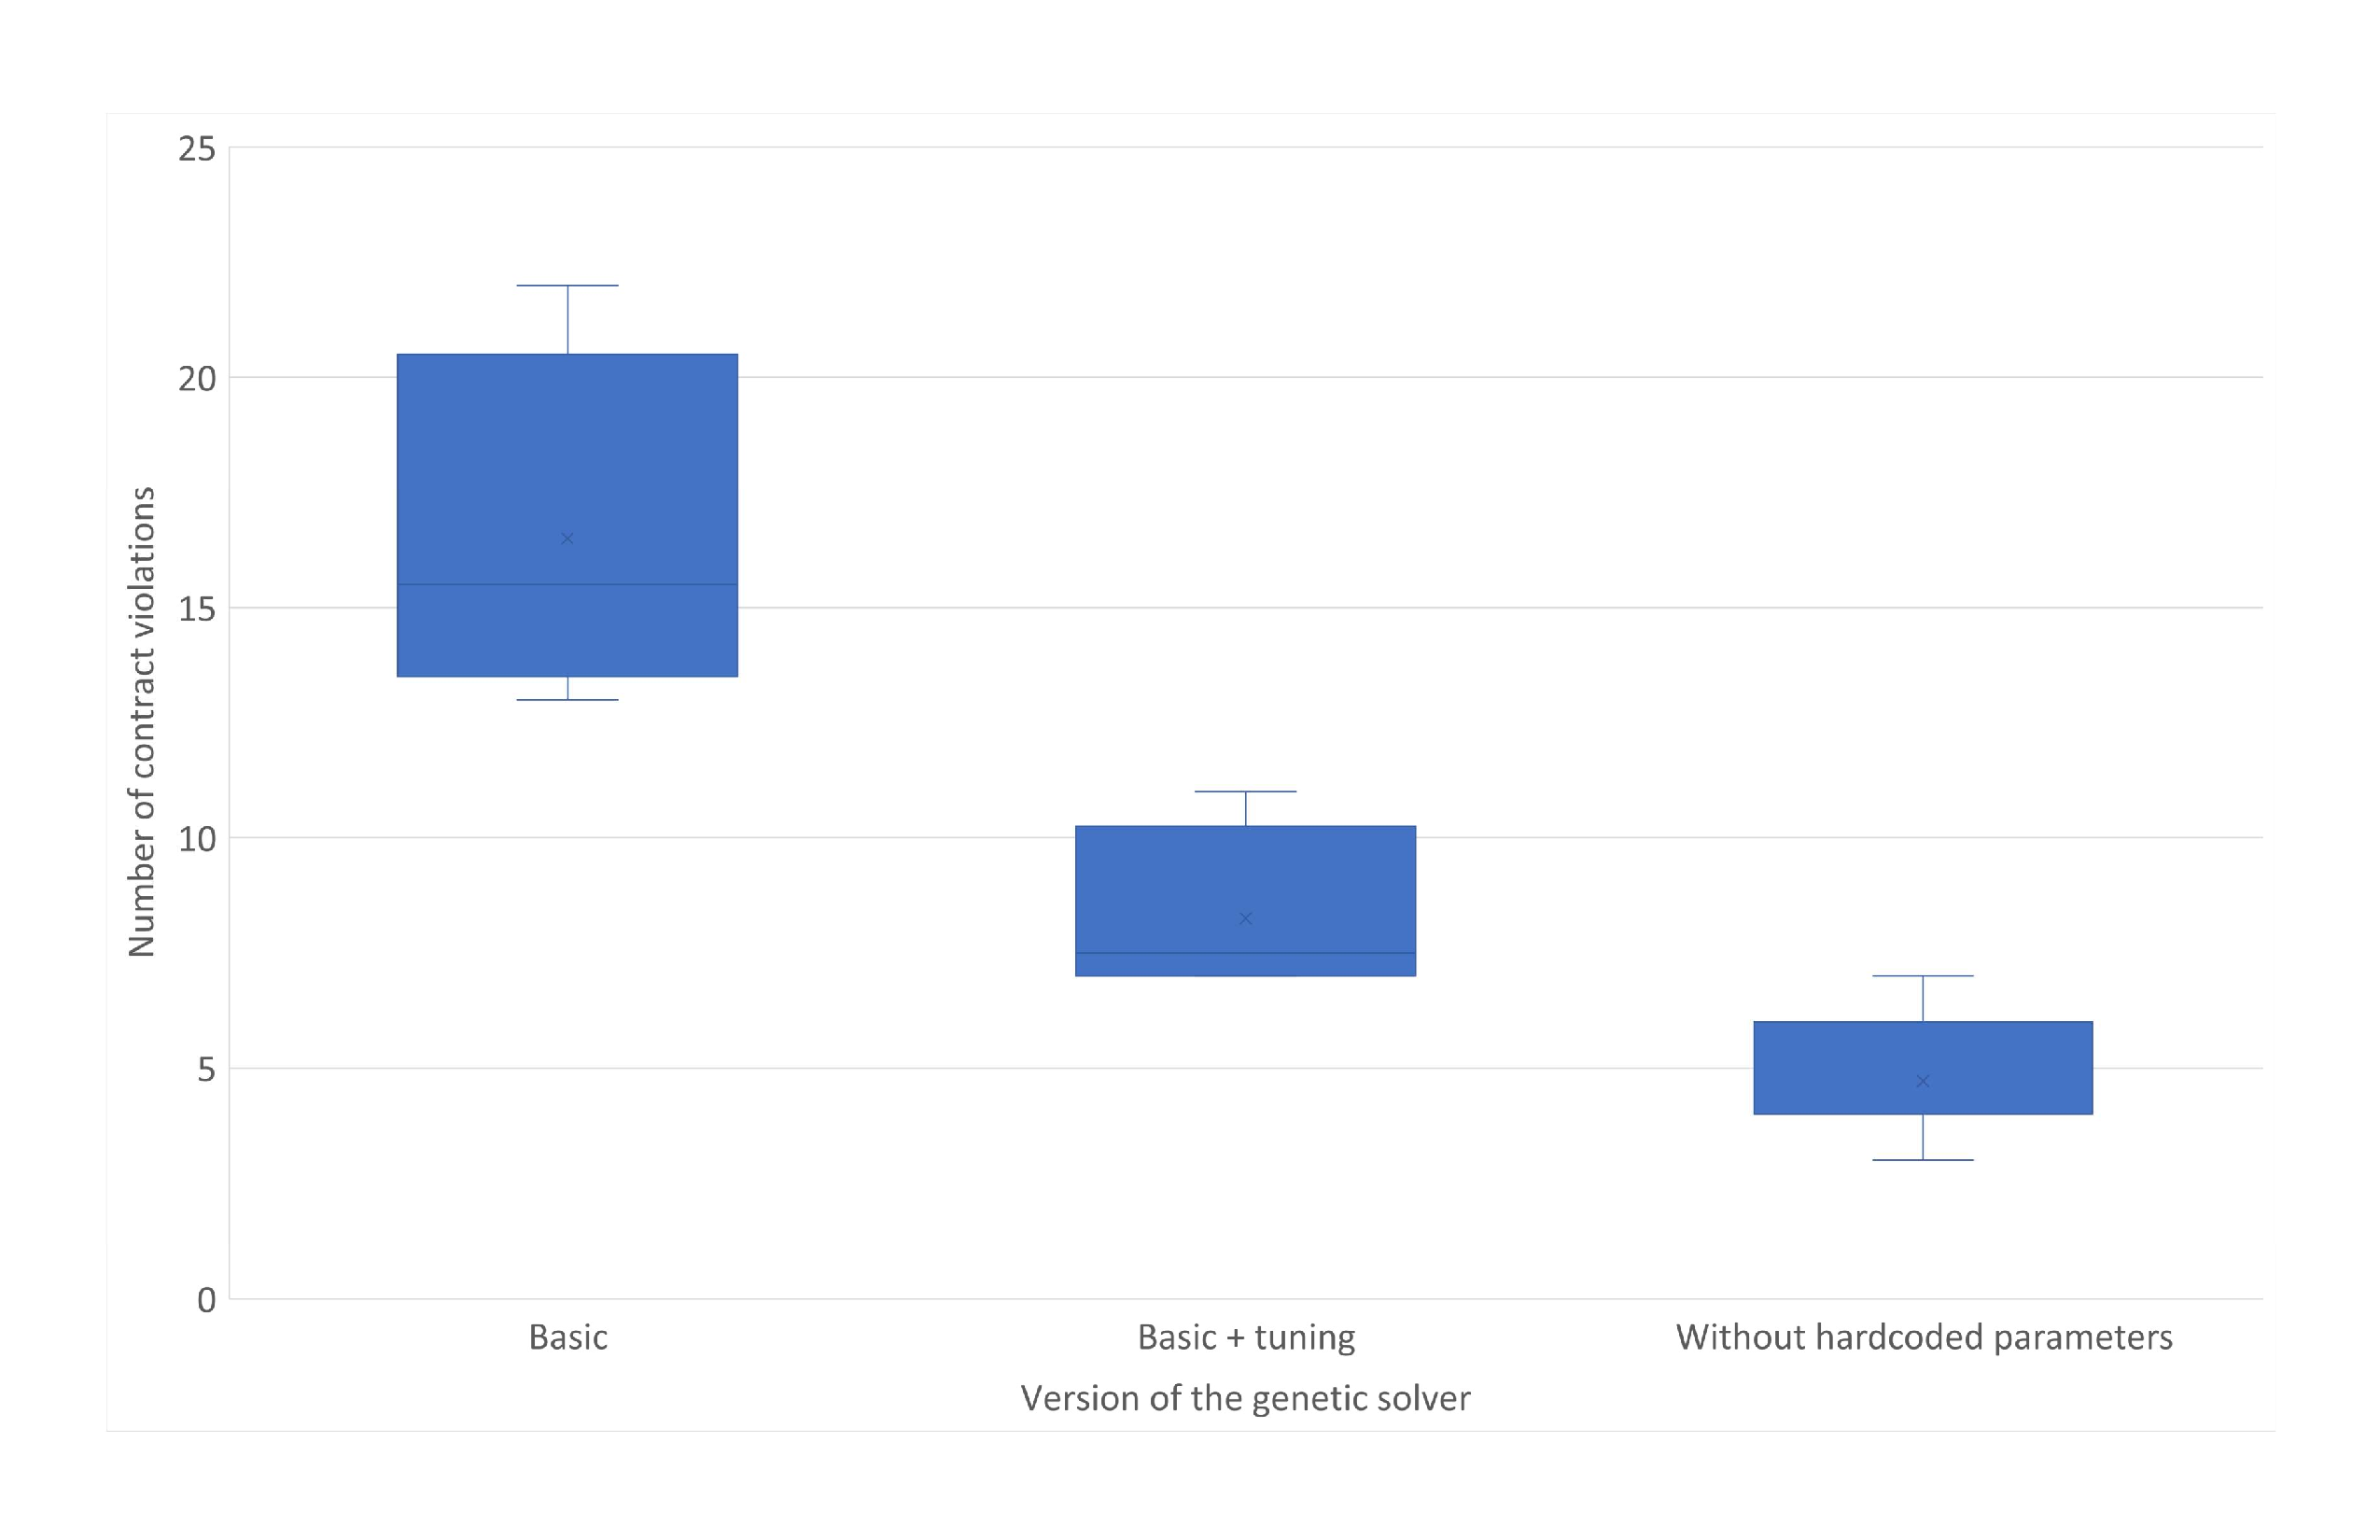
\includegraphics[width=\textwidth]{images/BoxPlotSolverNoHardcodedTuning.pdf}
	\caption[Boxplot with a number of contract violations for the genetic solver without hardcoded parameters in comparison with previous versions]{Boxplot with a number of contract violations for the genetic solver without hardcoded parameters in comparison with previous versions}
	\label{fig:boxplotsolverNoHardcodedTuning}
\end{figure}

This section shows how correctly selected parameter values affect the result of the algorithm in terms of solution validity. For the described problem without complex changes in the algorithm, we got a result which in the worst-case, gave a solution that is almost twice as good as the best solution in the B version of the genetic solver. However, parameter optimization is not enough to obtain valid solutions for the tasks described at the beginning of this chapter. 

\section{New Parameters}\label{sec:NP}

Since the parameter tuning from the previous steps do not give us valid results, we decided to use a parameter engineering approach.
Detailed analysis of crossover and mutation operators showed that the crossover point and the mutation points are coarse-grained. The principle how these points defines described in Section~\ref{sec:GeneticAlgorithmCrossover} and Section~\ref{sec:GeneticAlgorithmMutation}.

We add a few more parameters to crossover and mutation operators. These are probabilities, that allow change of the crossover/mutation points location in different ways in the Tree Shape Genotype.
There are:
\paragraph{\texttt{CrossoverOnRandomChildProbability}~(R14)~[0.0-1.0]} - the chance that crossover will occur on the random child or both children otherwise~(since the MQuAT problem constraints described in Section~\ref{sec:MQuATProblem}).
\paragraph{\texttt{CrossoverOnRandomLevelProbability}~(R15)~[0.0-1.0]} - the probability that describes a chance to do a crossover on random level of the tree, 
\paragraph{\texttt{CrossoverOnRandomRequestProbability}~(R16)~[0.0-1.0]} - the chance to do a crossover on random request,
\paragraph{\texttt{MutationOnRandomChildProbability}~(R17)~[0.0-1.0]} - the probability that describes a chance of mutation on a random child,
\paragraph{\texttt{MutationOnRandomLevelProbability}~(R18)~[0.0-1.0]} - the chance of mutation on a random level of the tree shape genotype.

The default value for there probabilities, except \texttt{Cross\-ov\-er\-On\-Ran\-dom\-Re\-qu\-est\-Pro\-ba\-bi\-li\-ty}~(R16), is 0.5. For the \texttt{CrossoverOnRandomRequestProbability}~(R16) is 0.0. These values we received empirically during developing.

This version~\footnote{commit: \href{https://git-st.inf.tu-dresden.de/mquat/mquat2/commit/817f7f1ef06f3acbbb4d5e24e32a26c5e6abc4b5}{817f7f1ef06f3acbbb4d5e24e32a26c5e6abc4b5}} of the genetic solver marked as \textbf{NP}(New Probabilities).

The set of parameters used during development is presented in Table~\ref{tab:Parameters_NP-T}. New parameters have the values described above. Furthermore, previously discussed parameters have values from the B version of the genetic solver. That means that all parameters are not tuned.

\begin{table}
	\centering
	\caption{Parameters of NP and NP-T versions of the genetic solver}\label{tab:Parameters_NP-T}
	\resizebox{\textwidth}{!}{
		\begin{tabular}{c c c c c c c c c c c c c c c c c}
			\hline
			\rotatebox{0}{Genetic solver} & \rotatebox{0}{\texttt{R1}} & \rotatebox{0}{\texttt{R3}} & \rotatebox{0}{\texttt{R4}} & \rotatebox{0}{\texttt{R5}} & \rotatebox{0}{\texttt{R6}} & \rotatebox{0}{\texttt{R7}} & \rotatebox{0}{\texttt{R8}}  & \rotatebox{0}{\texttt{R10}} & \rotatebox{0}{\texttt{R11}} & \rotatebox{0}{\texttt{R12}} & \rotatebox{0}{\texttt{R13}} &
			\rotatebox{0}{\texttt{R14}} &
			\rotatebox{0}{\texttt{R15}} &
			\rotatebox{0}{\texttt{R16}} &
			\rotatebox{0}{\texttt{R17}} &
			\rotatebox{0}{\texttt{R18}} \\
			\hline            
			NP & NSGA2 & 500 & 0.1 & 0.95 & 0.1 & 0.45 & 0.5 & 0.5 & 0.5 & 50 & 100 & 0.5 & 0.5 & 0.0 & 0.5 & 0.5 \\
			NP-T & NSGA2 & 2550 & 0.5 & 0.5 & 0.5 & 0.5 & 0.5 & 0.5 & 0.5 & 500 & 500 & 0.5 & 0.5 & 0.5 & 0.5 & 0.5 \\
			\hline
		\end{tabular}
	}
\end{table}

The result of the \textbf{NP} version of the genetic solver presented as boxplot in comparison with earlier versions~(\textbf{B}, \textbf{B-T}, \textbf{WHC-T}) shown in Figure~\ref{fig:boxplotsolverNewParameters}. If we compare the \textbf{B} and the \textbf{NP} versions, then both versions have non-optimized parameter values. The NP version has a minimal number of contract violations equal 3. It is \textbf{3} times less violations than in the best case if the \textbf{B} version. Moreover, this version of the genetic solver has results comparable to the results after parameter tuning in the \textbf{WHC-T} version. We can conclude, that better-designed parameters could also improve the target system. 

\begin{figure}
	\centering
	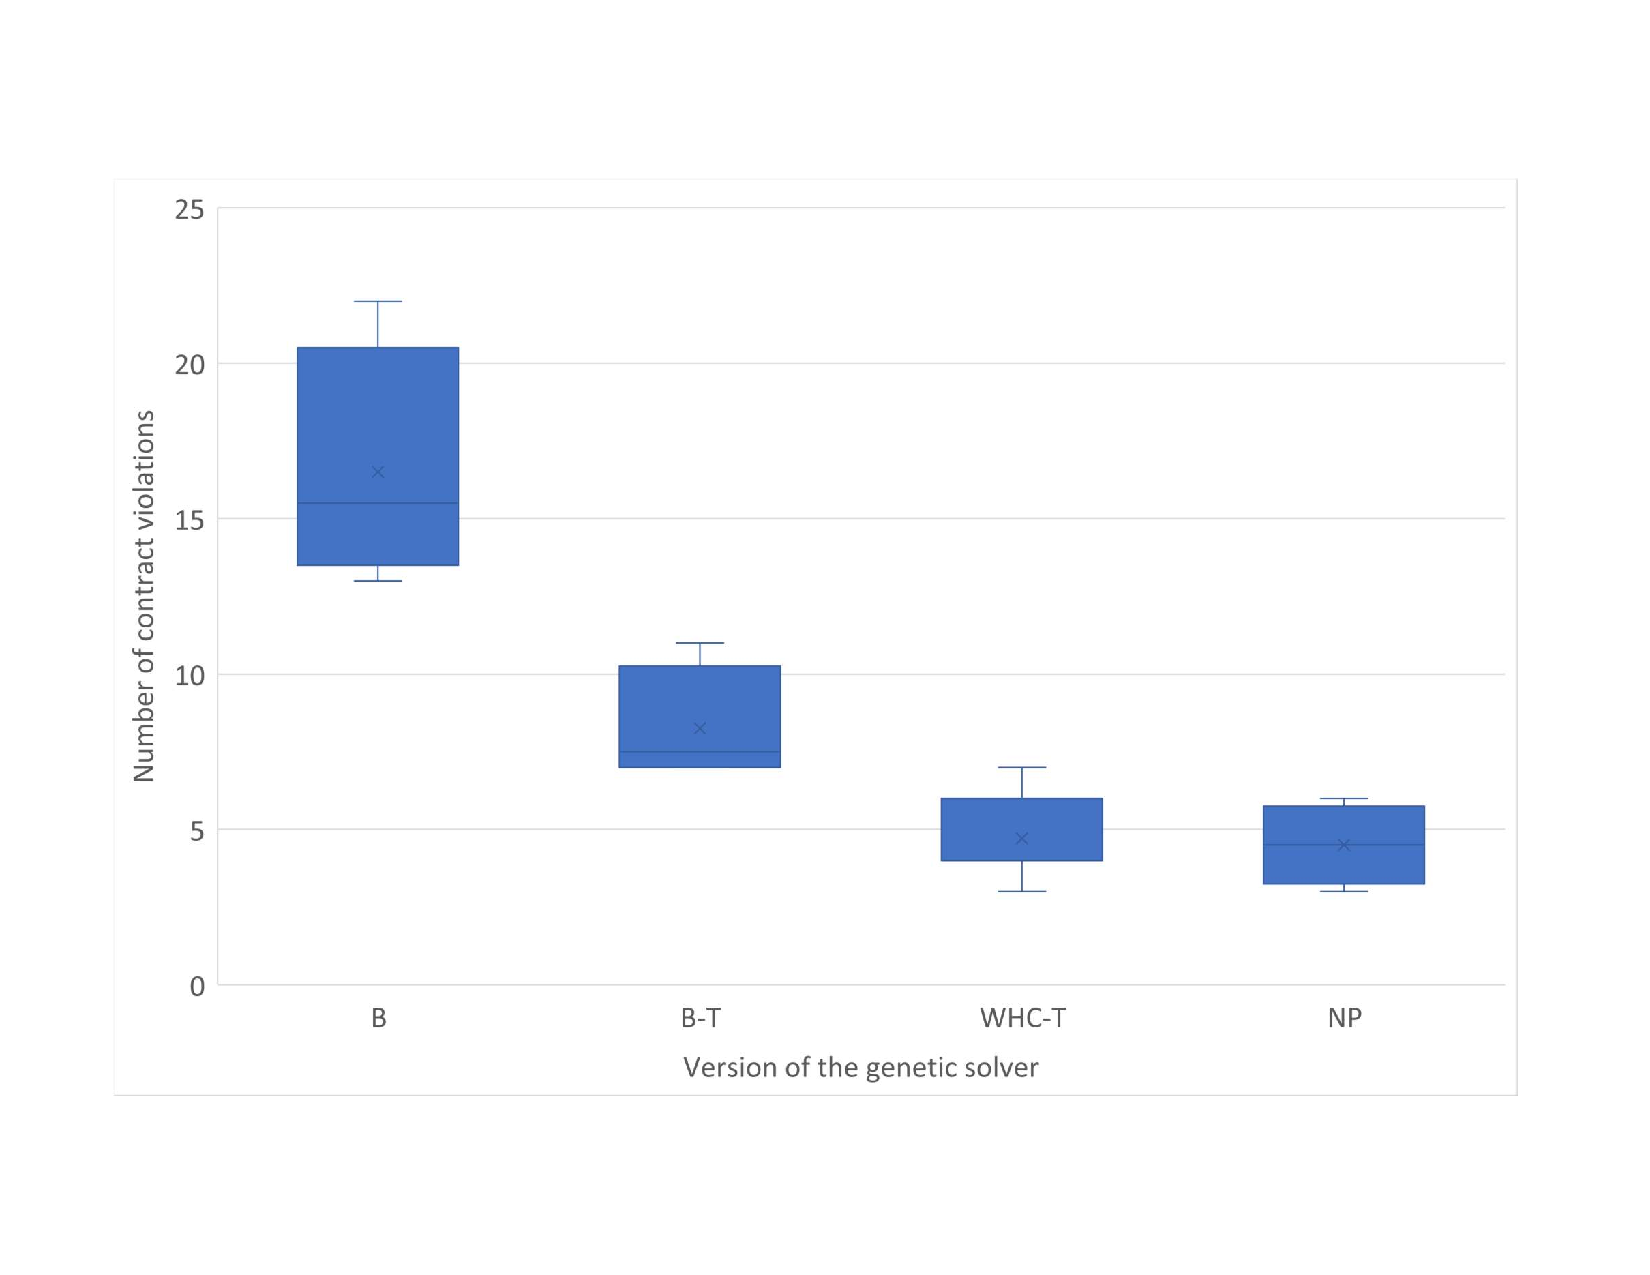
\includegraphics[width=\textwidth]{images/BoxPlotSolverNewParameters.pdf}
	\caption[Boxplot with a number of contract violations for the genetic solver with added probabilities without tuning in comparison with previous versions]{Boxplot with a number of contract violations for the genetic solver with added probabilities without tuning in comparison with previous versions}
	\label{fig:boxplotsolverNewParameters}
\end{figure}

After adding new parameters, we started BRISE to optimize all parameters. The optimized set of parameters is presented in Table~\ref{tab:Parameters_NP-T}. We marked the \textbf{NP} version with optimized set of parameters as \textbf{NP-T}(New Probabilities-Tuned)~\footnote{commit: \href{https://git-st.inf.tu-dresden.de/mquat/mquat2/commit/e103f52b3333900d61c6218a1f2ca811bca10289}{e103f52b3333900d61c6218a1f2ca811bca10289}}. As it was shown, parameter tuning with described parameters returns \textit{NSGA2} as a selector. Moreover, BRISE decide that optimized values of parameters located in the middle of the values range.

\begin{figure}
	\centering
	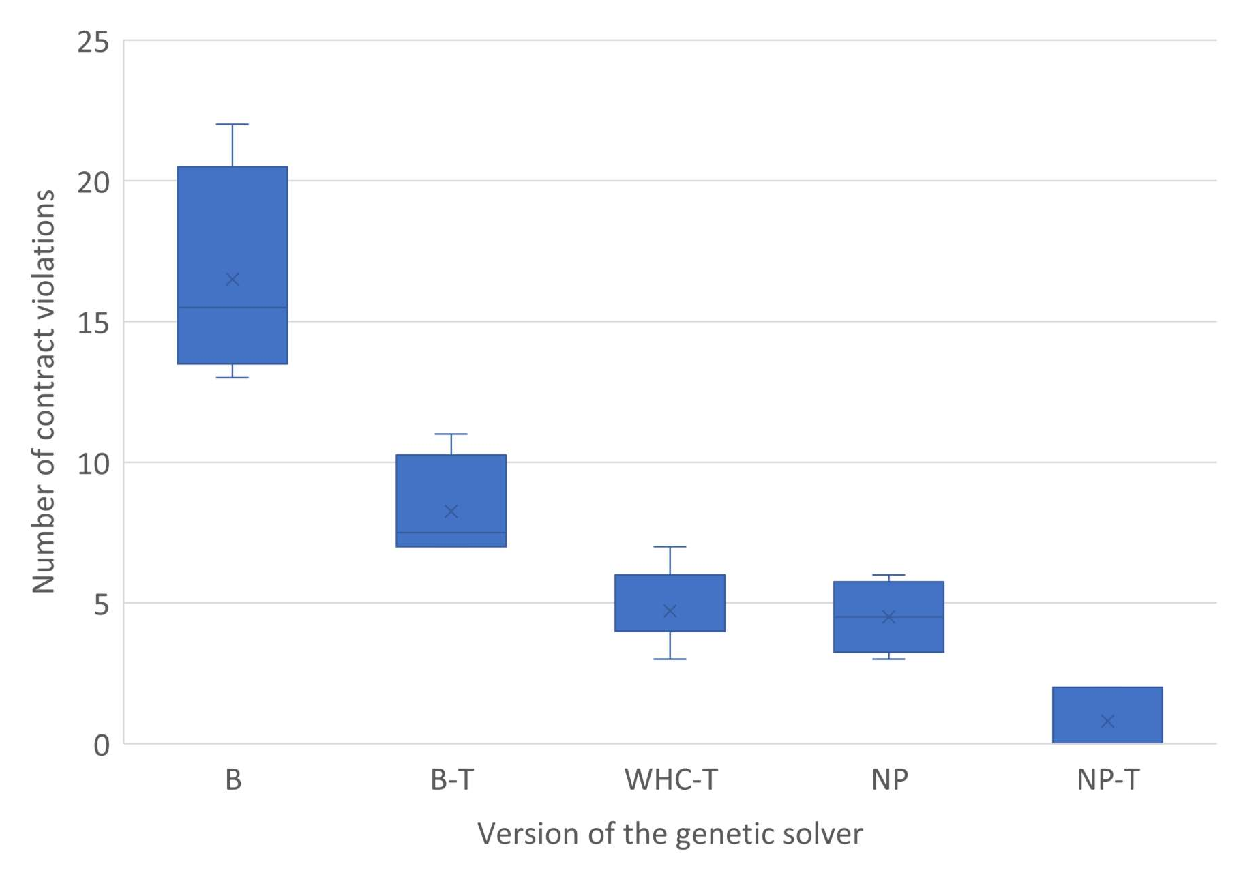
\includegraphics[width=\textwidth]{images/BoxPlotSolverNewParametersTuning.pdf}
	\caption[Boxplot with a number of contract violations for the genetic solver with added probabilities and tuned parameters in comparison with previous versions]{Boxplot with a number of contract violations for the genetic solver with added probabilities and tuned parameters in comparison with previous versions}
	\label{fig:boxplotsolverNewParametersTuning}
\end{figure}

Boxplots in Figure~\ref{fig:boxplotsolverNewParametersTuning} show the comparisons of the NP-T version of the genetic solver to earlier discussed versions~(\textbf{B}, \textbf{B-T}, \textbf{WHC-T}, \textbf{NT}). As shown, the combined approach of parameter engineering and parameter tuning gives a zero number of contract violations. It means that the \textbf{NP-T} version has a \textbf{valid} solution for the MQuAT problem described at the beginning of this chapter. Even the worth-case of the \textbf{NP-T} version with 2 contract violations is better than all versions presented in previous sections. \\ 

This section showed that the parameters thought out in the algorithm are as important as the values of these parameters. If the algorithm is not designed correctly, the tuning parameter may improve the results, but this may not be enough. But not all solutions of the \textbf{NP-T} version are valid. The reason for this is that all versions of the genetic solver that were previously discussed trap into the local optimum.  It could not get out because, at a certain moment, the majority of the individuals in the population becomes the same, and any newly created individual in most cases has worse value of the objective function. But we try to solve it.

\section{Simple parameter control}

The reason why all individuals become the same is the creation of the offspring. To create a new individual, the selector takes the best individuals. Crossover, takes two individuals from the selector, and performs a gene exchange, creating two new individuals. If these individuals give a worse solution, then the selector in the new iteration will drop them, but if they are better, it will take them to create new individuals. At a certain point, there will be a situation that the crossover occurs between two identical genotypes, which creates two identical to parents individuals. There is a case \texttt{1~-~mutationRate} that mutation will not happen, and two identical as parents individuals will be added to the population. It increases the number of identical elements and leads to the collapse of the genetic diversity of the population.

The idea of solving this issue is in internally changeable crossover rate. It changes the chance of the crossover depending on the number of identical individuals in a population. 
The principle of operation is as follows. After each iteration, the ratio of unique genotypes in the population is calculated. If the resulting number is smaller than the value of \texttt{PartOfUniqueIndividualsToStopCrossover}~(R19)~[0.0-1.0] parameter, then the probability of a crossover will be set to 0.0, and vice versa, the crossover rate returns its value if the ratio of unique genotypes in the population is bigger than the value of \texttt{PartOfUniqueIndividualsToReturnCrossover}~(R20)~[0.0-1.0] parameter.

The value for \texttt{PartOfUniqueIndividualsToStopCrossover} is 0.25 and\linebreak for \texttt{PartOfUniqueIndividualsToReturnCrossover} is 0.75.

The version of the genetic solver with internally changeable crossover rate marked as \textbf{ICCR}(Internally Changeable Crossover Rate)~\footnote{commit: \href{https://git-st.inf.tu-dresden.de/mquat/mquat2/commit/c89422c6e46a5f4e8bc09205df7713ad8fe6907c}{c89422c6e46a5f4e8bc09205df7713ad8fe6907c}} and tuned version~\footnote{commit: \href{https://git-st.inf.tu-dresden.de/mquat/mquat2/commit/128a6f2f844edd70d0e8ee616f09ac897cb86f4e}{128a6f2f844edd70d0e8ee616f09ac897cb86f4e}} was marked as \textbf{ICCR-T}(Internally Changeable Crossover Rate-Tuned).

The parameter sets used for both versions presented in Table~\ref{tab:Parameters_ICCR-T}. If we compare optimized values of parameters from previous section, we can see that \textit{NSGA2} selector changed to \textit{SPEA2}. All other values are the same.

\begin{table}
	\centering
	\caption{Parameters of ICCR and ICCR-T versions of the genetic solver}\label{tab:Parameters_ICCR-T}
	\resizebox{\textwidth}{!}{
		\begin{tabular}{c c c c c c c c c c c c c c c c c c c}
			\hline
			\rotatebox{0}{Genetic solver} & \rotatebox{0}{\texttt{R1}} & \rotatebox{0}{\texttt{R3}} & \rotatebox{0}{\texttt{R4}} & \rotatebox{0}{\texttt{R5}} & \rotatebox{0}{\texttt{R6}} & \rotatebox{0}{\texttt{R7}} & \rotatebox{0}{\texttt{R8}}  &  \rotatebox{0}{\texttt{R10}} & \rotatebox{0}{\texttt{R11}} & \rotatebox{0}{\texttt{R12}} & \rotatebox{0}{\texttt{R13}} &
			\rotatebox{0}{\texttt{R14}} &
			\rotatebox{0}{\texttt{R15}} &
			\rotatebox{0}{\texttt{R16}} &
			\rotatebox{0}{\texttt{R17}} &
			\rotatebox{0}{\texttt{R18}} &
			\rotatebox{0}{\texttt{R19}} &
			\rotatebox{0}{\texttt{R20}} \\
			\hline            
			ICCR & NSGA2 & 500 & 0.1 & 0.95 & 0.1 & 0.45 & 0.5 & 0.5 & 0.5 & 50 & 100 & 0.5 & 0.5 & 0.0 & 0.5 & 0.5 & 0.25 & 0.75 \\
			ICCR-T & SPEA2 & 2550 & 0.5 & 0.5 & 0.5 & 0.5 & 0.5 & 0.5 & 0.5 & 500 & 500 & 0.5 & 0.5 & 0.5 & 0.5 & 0.5 \\
			\hline
		\end{tabular}
	}
\end{table}


\begin{figure}
	\centering
	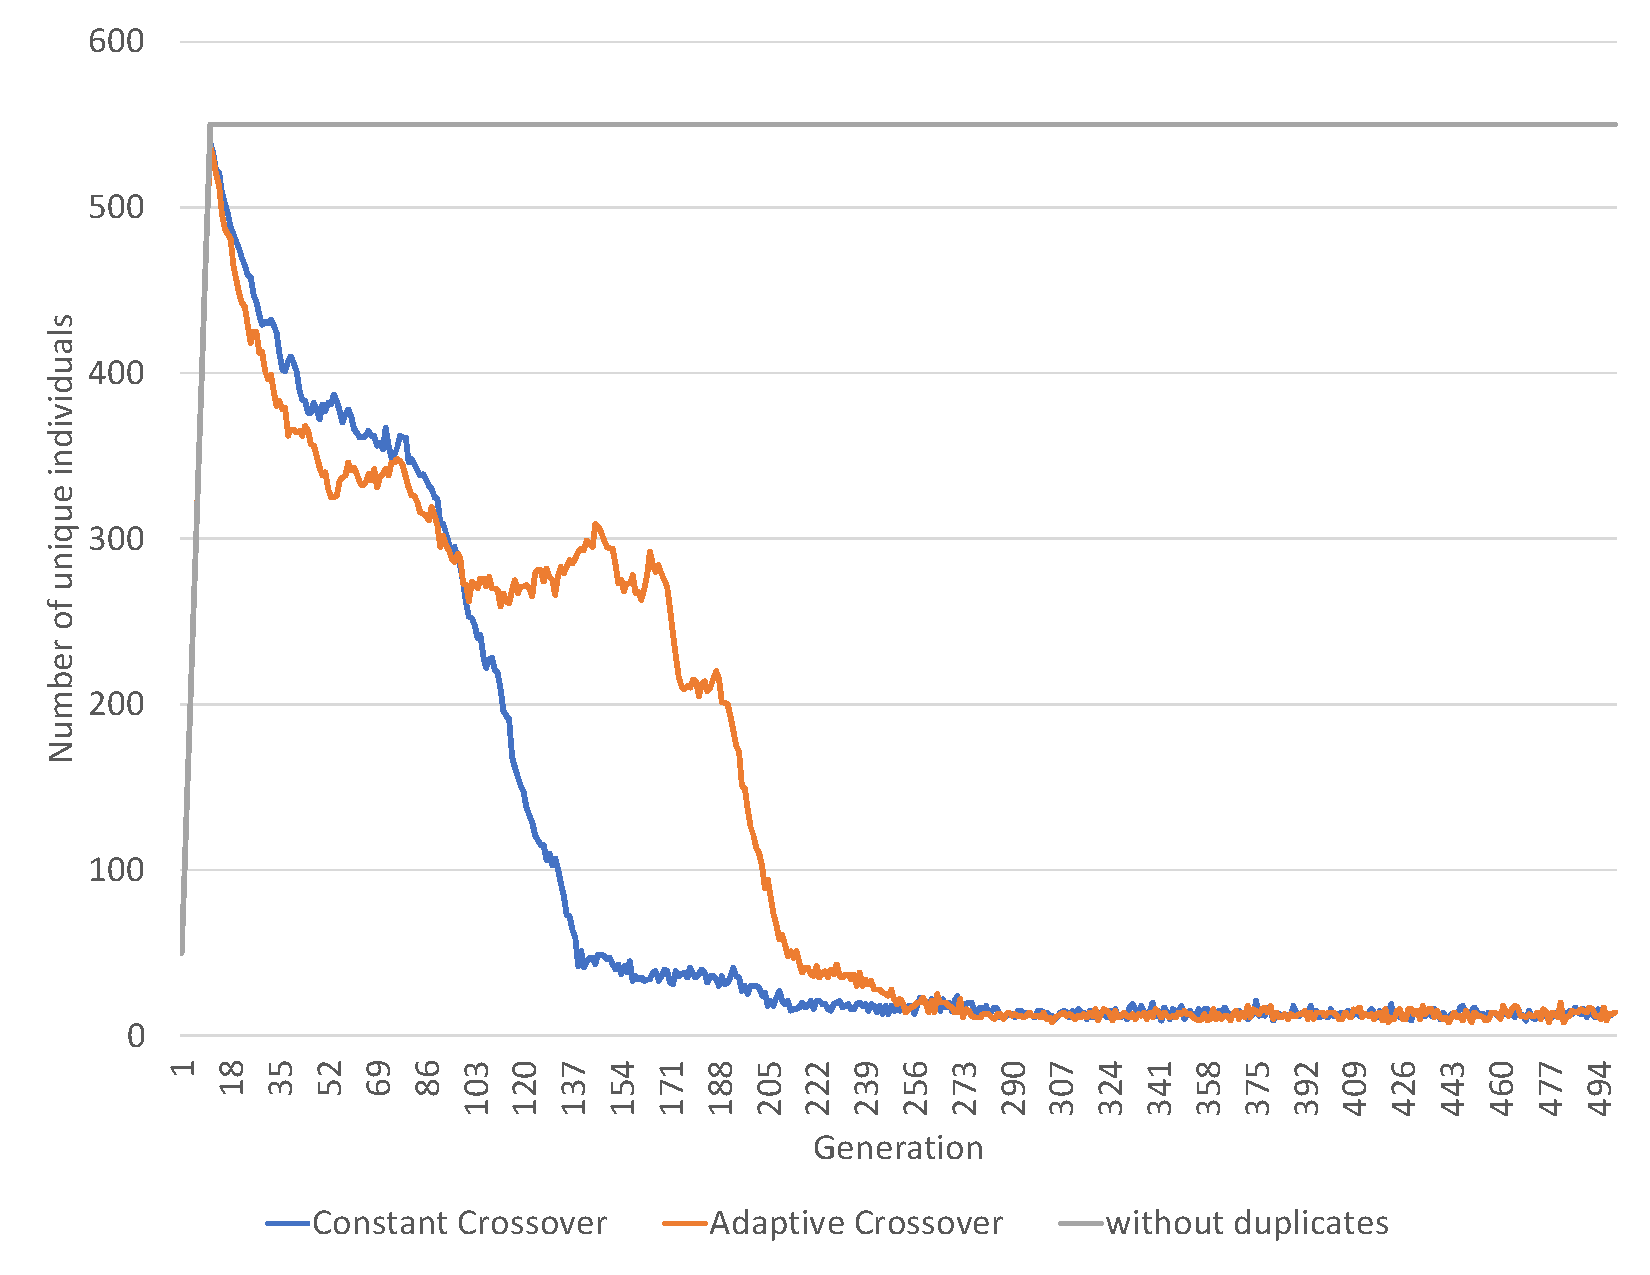
\includegraphics[width=\textwidth]{images/UniqIndividualsPerGeneration3.pdf}
	\caption[]{}
	\label{fig:UniqIndividualsPerGeneration3}
\end{figure} 


The internally changeable crossover rate slightly delay the collapse of the diversity of individuals in the population. Figure~\ref{fig:UniqIndividualsPerGeneration3} shows the deterioration in population diversity for a constant crossover rate and an internally changeable crossover rate.


The comparison of the results of \textbf{ICCR} and \textbf{ICCR-T} versions with all earlier discussed versions is presented as boxplots showed in Figure~\ref{fig:boxplotsolverAdaptiveCrossoverTuning}. The \textbf{ICCR} version gives better results than all untuned versions of the genetic solver. However, the range between max and min number of contract violations in the \textbf{ICCR} version is bigger than in the \textbf{NP} version.
The \textbf{ICCR} also better than tuned versions such as \textbf{B-T} and \textbf{WHC-T}, but worse than the \textbf{NP-T} version. The \textbf{ICCR-T} version as an \textbf{NP-T} version gives a valid solution, but in more like an exception case. The boxplot of the \textbf{ICCR-T} version also shows that parameter tuning for internally changeable parameters works not so efficient as for static parameters like in \textbf{NP} version, at least for the discussed problem. 

\begin{figure}
	\centering
	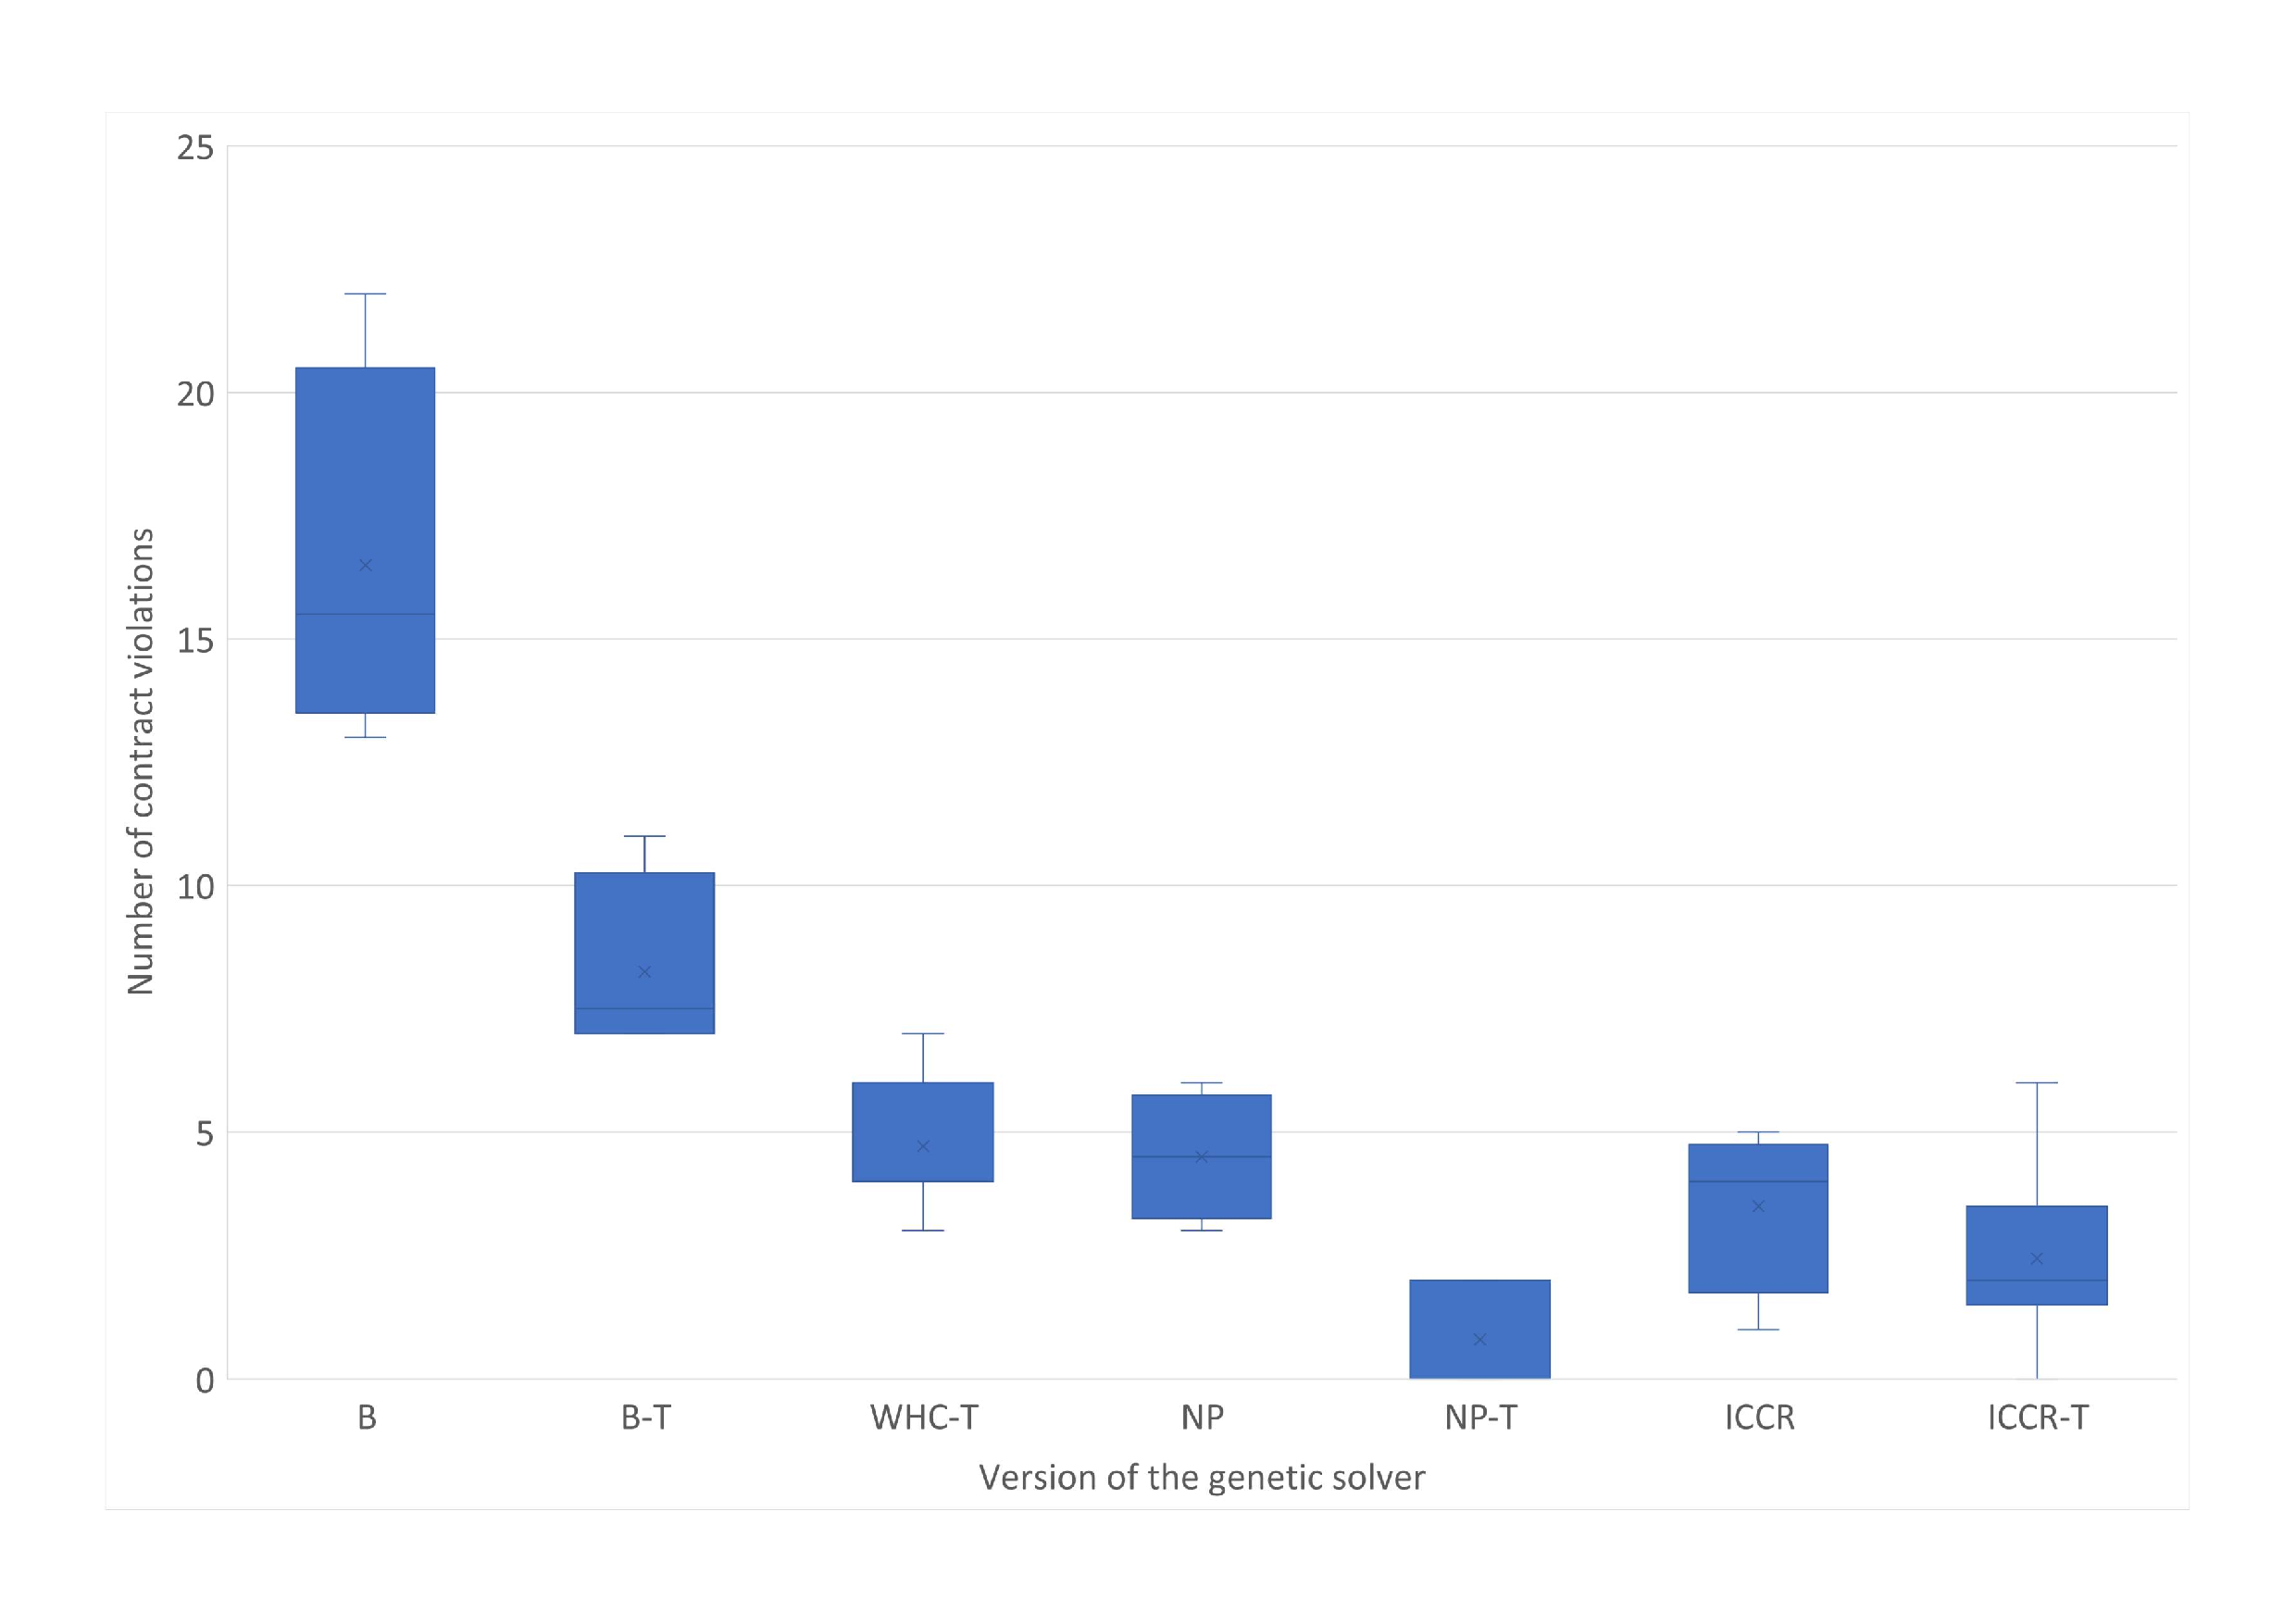
\includegraphics[width=\textwidth]{images/BoxPlotSolverAdaptiveCrossoverTuning.pdf}
	\caption[Boxplot with a number of contract violations for the genetic solver with internally changeable crossover rate in comparison with previously discussed versions]{Boxplot with a number of contract violations for the genetic solver with internally changeable crossover rate in comparison with previously discussed versions}
	\label{fig:boxplotsolverAdaptiveCrossoverTuning}
\end{figure}


This section shows that parameter control could improve the results and postpone stuck in a local optimum. However, parameter tuning for static parameters does not work so well on parameters that change their values during the run-time.                     

\section{Unique genotypes in a population}
\label{sec:WD}

Since the changeable crossover rate from the previous section only delays the collapse of the diversity of individuals in the population, we try a more radical solution. We block the possibility of adding to the population a new individual if the population already contains the same individual. It means that at any moment, the population will consist of unique individuals. In this version of the genetic solver, the use of the changeable crossover rate does not make any sense, so it was disabled, and a constant value was used.

Untuned version ot the genetic solver with blocked duplicates in the population marked as  \textbf{WD}~\footnote{commit: \href{https://git-st.inf.tu-dresden.de/mquat/mquat2/commit/1d79c50d7932c9216c653bf6d0354d990f6aecbc}{1d79c50d7932c9216c653bf6d0354d990f6aecbc}}~(Without Duplicates) and tuned version~\footnote{commit: \href{https://git-st.inf.tu-dresden.de/mquat/mquat2/commit/24504c77024ac383c77849c5121471e0f06ce913}{24504c77024ac383c77849c5121471e0f06ce913}} marked as \textbf{WD-T}~(Without Duplicates-Tuned).

The number of unique individuals in the population for the WD version presented in Figure~\ref{fig:UniqIndividualsPerGeneration3}. In each generation, after the initial population has been created, the number of unique elements in the population is not changing.



Parameters for both versions presented in Table~\ref{tab:Parameters_WD-T}.


\begin{table}
	\centering
	\caption{Parameters of WD and WD-T versions of the genetic solver}\label{tab:Parameters_WD-T}
	\resizebox{\textwidth}{!}{
		\begin{tabular}{c c c c c c c c c c c c c c c c c}
			\hline
			\rotatebox{0}{Genetic solver} & \rotatebox{0}{\texttt{R1}} & \rotatebox{0}{\texttt{R3}} & \rotatebox{0}{\texttt{R4}} & \rotatebox{0}{\texttt{R5}} & \rotatebox{0}{\texttt{R6}} & \rotatebox{0}{\texttt{R7}} & \rotatebox{0}{\texttt{R8}}  &  \rotatebox{0}{\texttt{R10}} & \rotatebox{0}{\texttt{R11}} & \rotatebox{0}{\texttt{R12}} & \rotatebox{0}{\texttt{R13}} &
			\rotatebox{0}{\texttt{R14}} &
			\rotatebox{0}{\texttt{R15}} &
			\rotatebox{0}{\texttt{R16}} &
			\rotatebox{0}{\texttt{R17}} &
			\rotatebox{0}{\texttt{R18}} \\
			\hline            
			WD & NSGA2 & 500 & 0.1 & 0.95 & 0.1 & 0.45 & 0.5 & 0.5 & 0.5 & 50 & 100 & 0.5 & 0.5 & 0.0 & 0.5 & 0.5 \\
			WD-T & SPEA2 & 1057 & 0.49 & 0.66 & 0.82 & 0.04 & 0.95 & 0.09 & 0.04 & 929 & 383 & 0.68 & 0.85 & 0.51 & 0.41 & 0.65 \\
			\hline
		\end{tabular}
	}
\end{table}

\begin{figure}
	\centering
	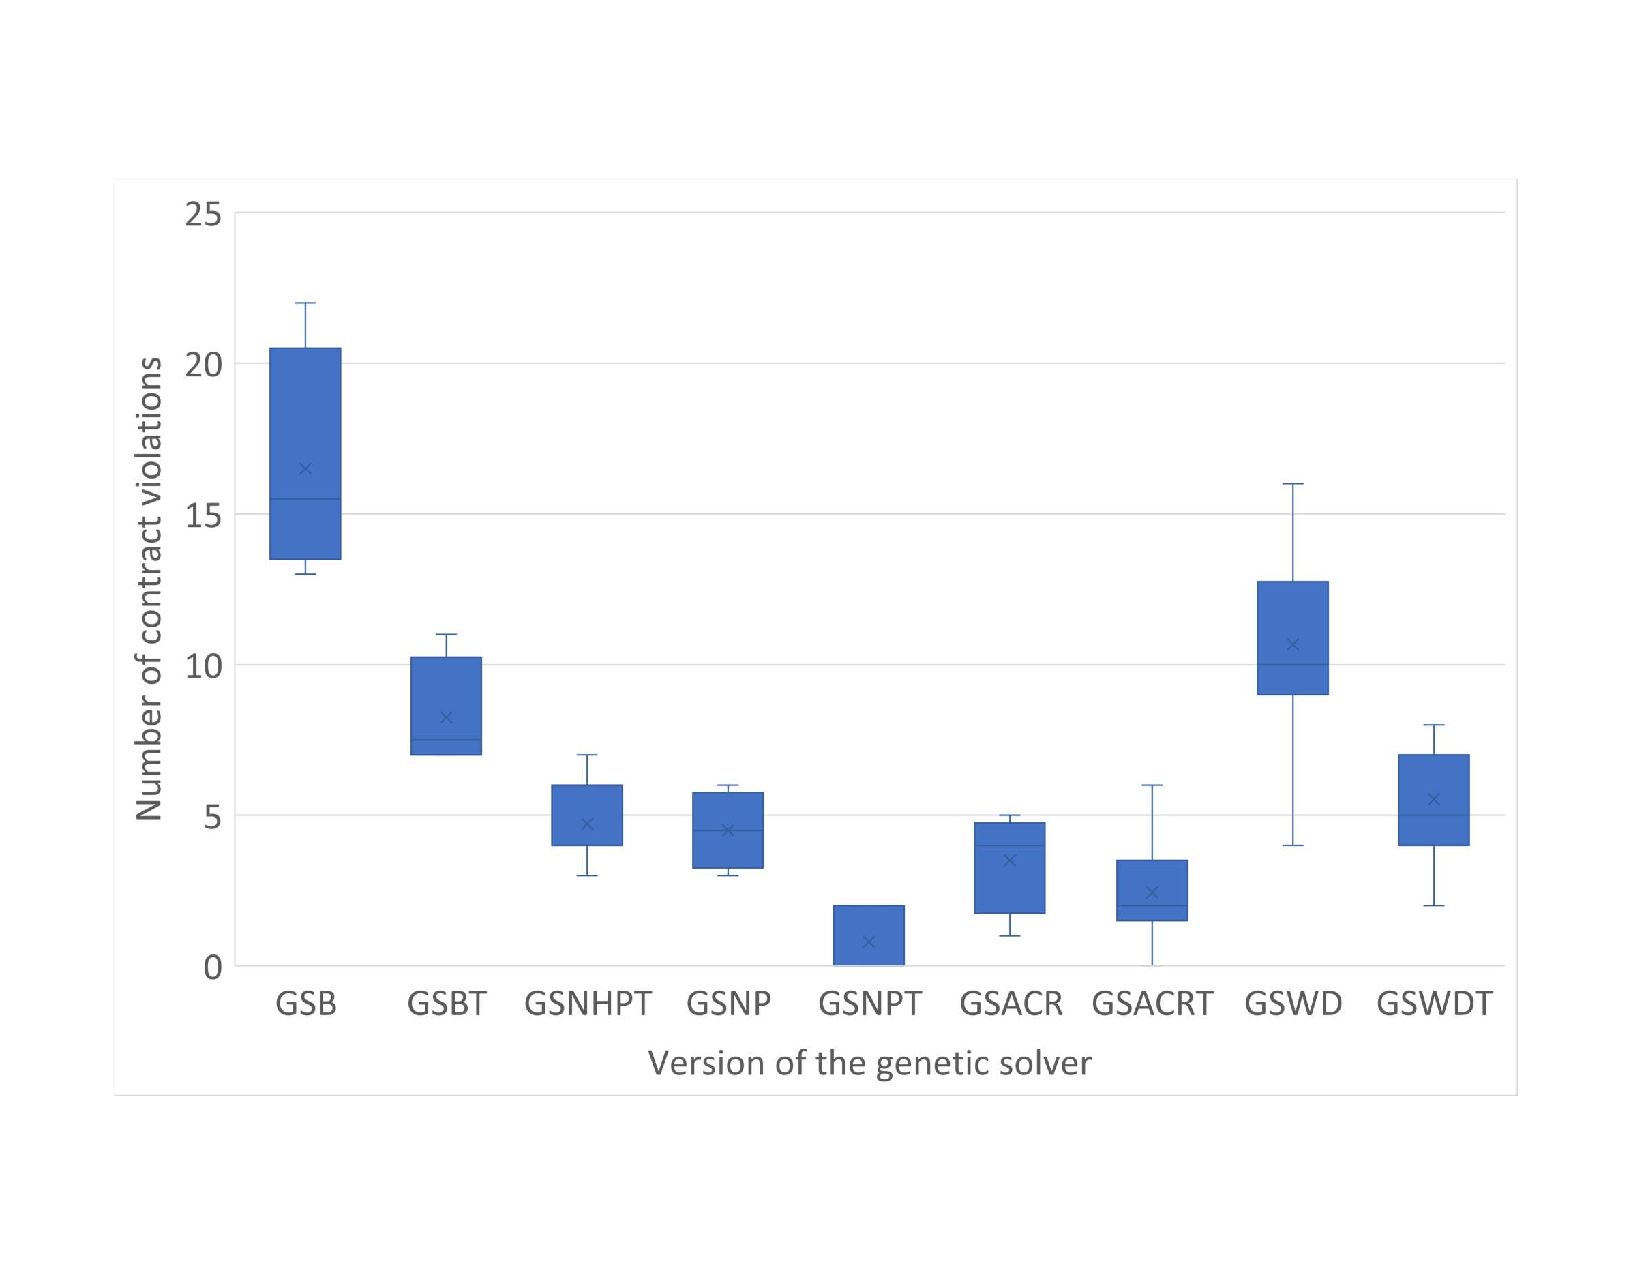
\includegraphics[width=\textwidth]{images/BoxPlotSolverNoDuplicates.pdf}
	\caption[Boxplot with a number of contract violations for the genetic solver without duplicates in the population in comparison with previous versions]{Boxplot with a number of contract violations for the genetic solver without duplicates in the population in comparison with previous versions}
	\label{fig:boxplotsolverNoDuplicates}
\end{figure} 

Figure~\ref{fig:boxplotsolverNoDuplicates} shows the results of this approach with and without parameter tuning. Obtained results show that the WD version of the genetic solver gives better results only in comparison to the B version and not always. The WD-T version gives better results with less range between min and max number of contract violations than WD. But it much worse than NP-T.

There are two main reasons why the results of this approach are much worse than previous versions. The first one is a calculation speed. It is slower than in previous versions. As a result, the number of created generations is lower. For the NP version, this number is 15177. For the WD version, this number is 2605, more than five times less according to our tests.

The second reason is a small number of "good" individuals selected to create offspring. This number is low because the selector could select the best individual from the population only once per selection. As a result, selected the best individual could give a few new individuals. Theoretically, the small value of the \texttt{mu} parameter could help. Nevertheless, BRISE gives the value of the \texttt{mu} parameter even higher than the default value. 

The conclusion of this idea is quite pessimistic because other approaches work better on this problem, but it may work better than others with different problems or on long term optimization.


\begin{table}
	\centering
	\caption{Parameters of NP and NP-T versions of the genetic solver}\label{tab:Parameters_all_versions}
	\resizebox{\textwidth}{!}{
		\begin{tabular}{c c c c c c c c c c c c c c c c c c c c}
			\hline
			\rotatebox{0}{Genetic solver} & \rotatebox{0}{\texttt{R1}} & \rotatebox{0}{\texttt{R3}} & \rotatebox{0}{\texttt{R4}} & \rotatebox{0}{\texttt{R5}} & \rotatebox{0}{\texttt{R6}} & \rotatebox{0}{\texttt{R7}} & \rotatebox{0}{\texttt{R8}}  & \rotatebox{0}{\texttt{R9}}  & \rotatebox{0}{\texttt{R10}} & \rotatebox{0}{\texttt{R11}} & \rotatebox{0}{\texttt{R12}} & \rotatebox{0}{\texttt{R13}} &
			\rotatebox{0}{\texttt{R14}} &
			\rotatebox{0}{\texttt{R15}} &
			\rotatebox{0}{\texttt{R16}} &
			\rotatebox{0}{\texttt{R17}} &
			\rotatebox{0}{\texttt{R18}} &
			\rotatebox{0}{\texttt{R19}} &
			\rotatebox{0}{\texttt{R20}} \\
			\hline            
			B & NSGA2 & 500 & \cellcolor{Gray} 0.1 & \cellcolor{Gray} 0.95 & \cellcolor{Gray} 0.1 & \cellcolor{Gray} 0.45 & \cellcolor{Gray} 0.5 & \cellcolor{Gray} 0.8 & \cellcolor{Gray} 0.5 & \cellcolor{Gray} 0.5 & \cellcolor{Gray} 50 & \cellcolor{Gray} 100 \\
			
			B-T & NSGA2 & 1533 & \cellcolor{Gray} 0.1 & \cellcolor{Gray} 0.95 & \cellcolor{Gray} 0.1 & \cellcolor{Gray} 0.45 & \cellcolor{Gray} 0.5 & \cellcolor{Gray} 0.8 & \cellcolor{Gray} 0.5 & \cellcolor{Gray} 0.5 & \cellcolor{Gray} 50 & \cellcolor{Gray} 100 \\    
			
			WHC-T & SPEA2 & 2014 & 0.98 & 0.95 & 0.58 & 0.02 & 0.64 & 0.3 & 0.95 & 0.17 & 79 & 266 \\
			
			NP & NSGA2 & 500 & 0.1 & 0.95 & 0.1 & 0.45 & 0.5 & & 0.5 & 0.5 & 50 & 100 & 0.5 & 0.5 & 0.0 & 0.5 & 0.5 \\
			
			NP-T & NSGA2 & 2550 & 0.5 & 0.5 & 0.5 & 0.5 & 0.5 & & 0.5 & 0.5 & 500 & 500 & 0.5 & 0.5 & 0.5 & 0.5 & 0.5 \\
			
			ICCR & NSGA2 & 500 & 0.1 & 0.95 & 0.1 & 0.45 & 0.5 & & 0.5 & 0.5 & 50 & 100 & 0.5 & 0.5 & 0.0 & 0.5 & 0.5 & 0.25 & 0.75 \\
			
			ICCR-T & SPEA2 & 2550 & 0.5 & 0.5 & 0.5 & 0.5 & 0.5 & & 0.5 & 0.5 & 500 & 500 & 0.5 & 0.5 & 0.5 & 0.5 & 0.5 & 0.5 & 0.5 \\
			
			WD & NSGA2 & 500 & 0.1 & 0.95 & 0.1 & 0.45 & 0.5 & & 0.5 & 0.5 & 50 & 100 & 0.5 & 0.5 & 0.0 & 0.5 & 0.5 \\
			
			WD-T & SPEA2 & 1057 & 0.49 & 0.66 & 0.82 & 0.04 & 0.95 & & 0.09 & 0.04 & 929 & 383 & 0.68 & 0.85 & 0.51 & 0.41 & 0.65 \\
			\hline
		\end{tabular}
	}
\end{table}
\todoR{Do I really need this table?}



\chapter{Evaluation and Analysis}

In the previous chapter, a few approaches that could improve the genetic solver were presented.
The best results give a combination of the genetic solver with added probabilities and parameter tuning.
Other methods like a changeable crossover rate or population without duplicated individuals have less effect on the results.

However, we get valid results only for one problem. What if the problem will be smaller or bigger?
The evaluation was done to find out how all approaches work with different problem sizes. 

\section{Evaluation}
\label{sec:evaluation}

To evaluate the genetic solver, we performed a benchmark. The benchmark set consists of 36 problems. Each problem has different parameters that describe it.
All parameters are:
\begin{itemize}
	\item Software variants - [2, 4] ,
	\item Number of requests - [1, 2, 4],
	\item Component tree depth - [2, 3, 4],
	\item  Resources ratio - [50, 100],
	\item timeout to solve the problem: 5 minutes.
\end{itemize}

This set was tested with several versions of the genetic solver:

\begin{itemize}
	\item basic (B),
	\item basic with tuned parameters (B-T),
	\item without hard-coded parameters and tuning (WHC-T) 
	\item with added parameters (NP),
	\item with added parameters and tuning (NP-T),
	\item with internally changeable crossover rate (ICCR),
	\item with internally changeable crossover rate and tuning (ICCR-T),
	\item without duplicates in the population (WD),
	\item without duplicates in the population and tuning (WD-T).
\end{itemize}

Each version of the genetic solver tries five times to solve each problem.

The benchmark set was run on an Intel Core i7-8700 CPU machine with 64Gb of memory using Fedora Server 29 and OpenJDK 1.8.0 201-b09.

Benchmark trying so solve each task, if a solution was valid, genetic solver start to solve the next problem. If, after five attempts, the genetic solver did not find a valid solution, it proceeded to the next problem.

\begin{figure}
	\centering
	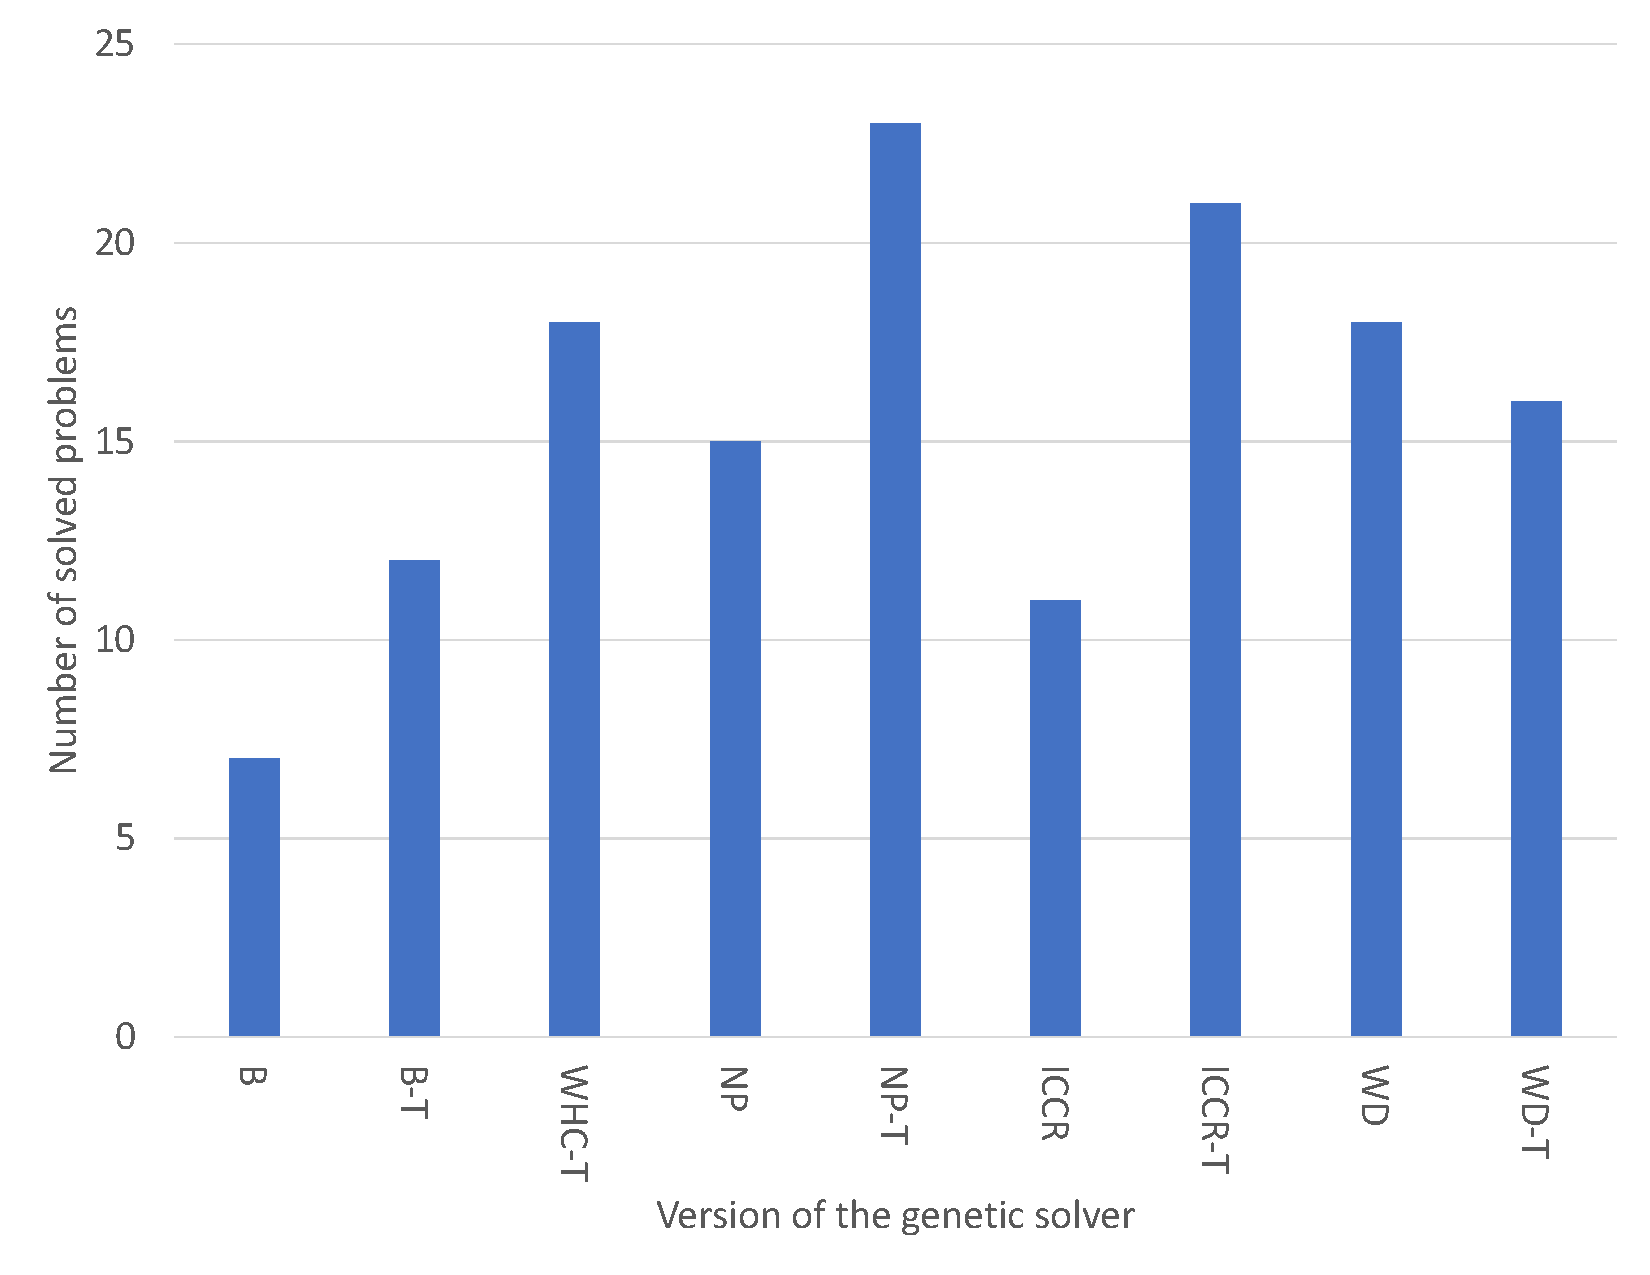
\includegraphics[width=\textwidth]{images/EvaluationNumberOfSolvedProblems.pdf}
	\caption[Number of problems for each version of the genetic solver]{Number of solved problems for each version of the genetic solver}
	\label{fig:EvaluationNumberOfSolvedProblems}
\end{figure}

Figure~\ref{fig:EvaluationNumberOfSolvedProblems} results of the benchmark. For each version of the genetic solver, a vertical bar was built. The height of the bar shows the number of solved problems from the benchmark set. The B version solved the least of problems than any other version. Almost in all cases, parameter tuning increases the number of solved problems. It also confirms the answer to \textbf{RQ1}. 

The comparison of B-T, WHC-T, and NP versions shows that the NP bar is higher than B-T but lower than WHC-T. This comparison confirms the first conclusion from Section~\ref{sec:NP}, that well-designed parameters are important for any algorithm. The combination of parameter engineering and parameter tuning in NP-T gives the best results. The same situation was for one problem in the previous chapter~(Figure~\ref{fig:boxplotsolverNoDuplicates}). 

The WD-T gives worse results than the untuned version. The possible reason for such results is a high value of the \texttt{meu}~(R6) parameter. The result of the benchmark for the ICCR-T version contradicts the results obtained in the last section because the parameter tuning of the ICCR version gives the biggest improvement. In general, benchmark results for a set of 36 MQuAT problems correspond to the results for one problem.

The benchmark also shows that no one version of the genetic solver solved all problems from the set. Table~\ref{tab:ProblemsColorCoding} shows the results of the benchmark in the context of a solved or unsolved problem. Each row describes the result for a specified problem. The problem numbers contain in column \textit{Problem Id}. Black filled cell means that solver solved the problem. Table~\ref{tab:ProblemsColorCoding} also shows ids of problems that unsolved by all versions of the genetic solver.

\begin{table}
	\caption{Problem color coding}\label{tab:ProblemsColorCoding}
	\resizebox{0.8\textwidth}{!}{
	\begin{minipage}[t]{0.5\linewidth}
		\begin{tabular}[t]{c | c | c | c | c | c | c | c | c | c |}
			\rotatebox{90}{Problem Id} & \rotatebox{90}{B} & \rotatebox{90}{B-T} & \rotatebox{90}{WHC-T} & \rotatebox{90}{NP} & \rotatebox{90}{NP-T} & \rotatebox{90}{ICCR} & \rotatebox{90}{ICCR-T} & \rotatebox{90}{WD} & \rotatebox{90}{WD-T} \\
			\hline            
			1 & $\blacksquare$ & $\blacksquare$ & $\blacksquare$ & $\blacksquare$ & $\blacksquare$ & $\blacksquare$ & $\blacksquare$ & $\blacksquare$ & $\blacksquare$ \\ 
			2 & $\square$ & $\square$ & $\blacksquare$ & $\square$ & $\blacksquare$ & $\square$ & $\square$ & $\blacksquare$ & $\blacksquare$  \\
			3 & $\square$ & $\square$ & $\square$ & $\square$ & $\blacksquare$ & $\square$ & $\square$ & $\blacksquare$ & $\square$  \\
			4 & $\square$ & $\blacksquare$ & $\blacksquare$ & $\blacksquare$ & $\blacksquare$ & $\blacksquare$ & $\blacksquare$ & $\blacksquare$ & $\blacksquare$ \\
			5 & $\square$ & $\square$ & $\square$ & $\square$ & $\blacksquare$ & $\square$ & $\blacksquare$ & $\square$ & $\square$ \\
			6 & $\square$ & $\square$ & $\square$ & $\square$ & $\square$ & $\square$ & $\square$ & $\square$ & $\square$ \\
			7 & $\square$ & $\blacksquare$ & $\blacksquare$ & $\blacksquare$ & $\blacksquare$ & $\square$ & $\blacksquare$ & $\blacksquare$ & $\blacksquare$\\
			8 & $\square$ & $\square$ & $\square$ & $\square$ & $\square$ & $\square$ & $\square$ & $\square$ & $\square$ \\
			9 & $\square$ & $\square$ & $\square$ & $\square$ & $\square$ & $\square$ & $\square$ & $\square$ & $\square$ \\
			10 & $\blacksquare$ & $\blacksquare$ & $\blacksquare$ & $\blacksquare$ & $\blacksquare$ & $\blacksquare$ & $\blacksquare$ & $\blacksquare$ & $\blacksquare$ \\
			11 & $\square$ & $\square$ & $\blacksquare$ & $\blacksquare$ & $\blacksquare$ & $\blacksquare$ & $\blacksquare$ & $\blacksquare$ & $\blacksquare$ \\
			12 & $\square$ & $\square$ & $\square$ & $\square$ & $\blacksquare$ & $\square$ & $\blacksquare$ & $\blacksquare$ & $\square$  \\
			13 & $\blacksquare$ & $\blacksquare$ & $\blacksquare$ & $\blacksquare$ & $\blacksquare$ & $\blacksquare$ & $\blacksquare$ & $\blacksquare$ & $\blacksquare$ \\
			14 & $\square$ & $\square$ & $\square$ & $\square$ & $\blacksquare$ & $\square$ & $\blacksquare$ & $\square$ & $\square$  \\
			15 & $\square$ & $\square$ & $\square$ & $\square$ & $\square$ & $\square$ & $\square$ & $\square$ & $\square$ \\
			16 & $\square$ & $\blacksquare$ & $\blacksquare$ & $\blacksquare$ & $\blacksquare$ & $\square$ & $\blacksquare$ & $\square$ & $\blacksquare$ \\
			17 & $\square$ & $\square$ & $\square$ & $\square$ & $\square$ & $\square$ & $\square$ & $\square$ & $\square$ \\
			18 & $\square$ & $\square$ & $\square$ & $\square$ & $\square$ & $\square$ & $\square$ & $\square$ & $\square$ \\
			\hline
		\end{tabular} %
	\end{minipage}
	%\setlength{\tabcolsep}{0.05cm}
	%\renewcommand{\arraystretch}{0}
	\begin{minipage}[t]{0.49\linewidth}
		\begin{tabular}[t]{c | c | c | c | c | c | c | c | c | c}
			\rotatebox{90}{Problem Id} & \rotatebox{90}{B} & \rotatebox{90}{B-T} & \rotatebox{90}{WHC-T} & \rotatebox{90}{NP} & \rotatebox{90}{NP-T} & \rotatebox{90}{ICCR} & \rotatebox{90}{ICCR-T} & \rotatebox{90}{WD} & \rotatebox{90}{WD-T} \\
			\hline            
			19 & $\blacksquare$ & $\blacksquare$ & $\blacksquare$ & $\blacksquare$ & $\blacksquare$ & $\blacksquare$ & $\blacksquare$ & $\blacksquare$ & $\blacksquare$\\
			20 & $\square$ & $\square$ & $\blacksquare$ & $\blacksquare$ & $\blacksquare$ & $\blacksquare$ & $\blacksquare$ & $\blacksquare$ & $\blacksquare$ \\
			21 & $\square$ & $\square$ & $\square$ & $\square$ & $\blacksquare$ & $\square$ & $\blacksquare$ & $\square$ & $\square$ \\
			22 & $\blacksquare$ & $\blacksquare$ & $\blacksquare$ & $\square$ & $\blacksquare$ & $\blacksquare$ & $\blacksquare$ & $\blacksquare$ & $\blacksquare$ \\
			23 & $\square$ & $\square$ & $\blacksquare$ & $\blacksquare$ & $\blacksquare$ & $\square$ & $\blacksquare$ & $\blacksquare$ & $\square$ \\
			24 & $\square$ & $\square$ & $\square$ & $\square$ & $\square$ & $\square$ & $\square$ & $\square$ & $\square$ \\
			25 & $\square$ & $\square$ & $\blacksquare$ & $\blacksquare$ & $\blacksquare$ & $\square$ & $\blacksquare$ & $\square$ & $\blacksquare$ \\
			26 & $\square$ & $\square$ & $\square$ & $\square$ & $\square$ & $\square$ & $\square$ & $\square$ & $\square$ \\
			27 & $\square$ & $\square$ & $\square$ & $\square$ & $\square$ & $\square$ & $\square$ & $\square$ & $\square$ \\
			28 & $\blacksquare$ & $\blacksquare$ & $\blacksquare$ & $\blacksquare$ & $\blacksquare$ & $\blacksquare$ & $\blacksquare$ & $\blacksquare$ & $\blacksquare$ \\
			29 & $\square$ & $\blacksquare$ & $\blacksquare$ & $\blacksquare$ & $\blacksquare$ & $\blacksquare$ & $\blacksquare$ & $\blacksquare$ & $\blacksquare$ \\
			30 & $\square$ & $\square$ & $\square$ & $\square$ & $\square$ & $\square$ & $\square$ & $\square$ & $\square$ \\
			31 & $\blacksquare$ & $\blacksquare$ & $\blacksquare$ & $\blacksquare$ & $\blacksquare$ & $\blacksquare$ & $\blacksquare$ & $\blacksquare$ & $\blacksquare$ \\
			32 & $\square$ & $\square$ & $\blacksquare$ & $\blacksquare$ & $\blacksquare$ & $\square$ & $\blacksquare$ & $\blacksquare$ & $\square$ \\ 
			33 & $\square$ & $\square$ & $\square$ & $\square$ & $\square$ & $\square$ & $\square$ & $\square$ & $\square$ \\
			34 & $\square$ & $\blacksquare$ & $\blacksquare$ & $\square$ & $\blacksquare$ & $\square$ & $\blacksquare$ & $\blacksquare$ & $\blacksquare$ \\
			35 & $\square$ & $\square$ & $\square$ & $\square$ & $\square$ & $\square$ & $\square$ & $\square$ & $\square$ \\
			36 & $\square$ & $\square$ & $\square$ & $\square$ & $\square$ & $\square$ & $\square$ & $\square$ & $\square$ \\
			\hline
		\end{tabular} %
	\end{minipage}
	}
	\mbox{$\blacksquare$: solved, $\square$: unsolved}
\end{table}

Unsolved tasks are presented in Table~\ref{tab:UnsolvedProblems}. It shows parameters that specified the problem. We can see, there are a few types of unsolved problems are exist. All versions of the genetic solver could not solve the problem that contains two or more requests, and the depth is three or more. The exception for this definition is a problem number 30. It has one request and depth four, but it also has variants four and resources - 100 and genetic solvers could not solve it.

\begin{itemize}
	\item Software variants - [2, 4] ,
	\item Number of requests - [1, 2, 4],
	\item Component tree depth - [2, 3, 4],
	\item Resources ratio - [50, 100],
	\item timeout to solve the problem: 5 minutes.
\end{itemize}

\begin{table}
	\centering
	\caption{Not solved problems}\label{tab:UnsolvedProblems}
	%\resizebox{0.6\textwidth}{!}{
		\begin{tabular}{c c c c c}
			\hline
			Problem Id & Software variants & umber of requests & Component tree depth & Resources ratio \\
			\hline            
			6 & 2 & 2 & 4 & 50 \\
			8 & 2 & 4 & 3 & 50 \\
			9 & 2 & 4 & 4 & 50 \\
			15 & 2 & 2 & 4 & 100 \\
			17 & 2 & 4 & 3 & 100 \\
			18 & 2 & 4 & 4 & 100 \\
			24 & 4 & 2 & 4 & 50 \\
			26 & 4 & 4 & 3 & 50 \\
			27 & 4 & 4 & 4 & 50 \\
			30 & 4 & 1 & 4 & 100 \\
			33 & 4 & 2 & 4 & 100 \\
			35 & 4 & 4 & 3 & 100 \\
			36 & 4 & 4 & 4 & 100 \\
			\hline
		\end{tabular}
	%}
\end{table}

If a genetic solver could solve some problems, then solutions have a quality.
Let us now discuss the quality of the received results. Figure~\ref{fig:EnergyPercentage} shows the percentage of the deviation from the optimum for problems that solved by all versions of the genetic solver. The optimum values for problems received by the ILP solver. If the percentage of the deviation is zero, that means that the received solution is \textbf{optimal}. The max deviation is near 30\% for the B version with problem 31. However, other versions give solutions with deviation from optimal that less than 10\% or even optimal solutions for the NP-T version. There are high deviations from optimum in problems number 13 for tuned versions of the genetic solver such as B-T, NP-T, ICCR-T, and WD-T. Nevertheless, WHC-T and untuned versions give a near-optimal solution with minimal deviation. The ICCR version gives a much higher percentage of deviation than other versions in problem 19.

\begin{figure}
	\centering
	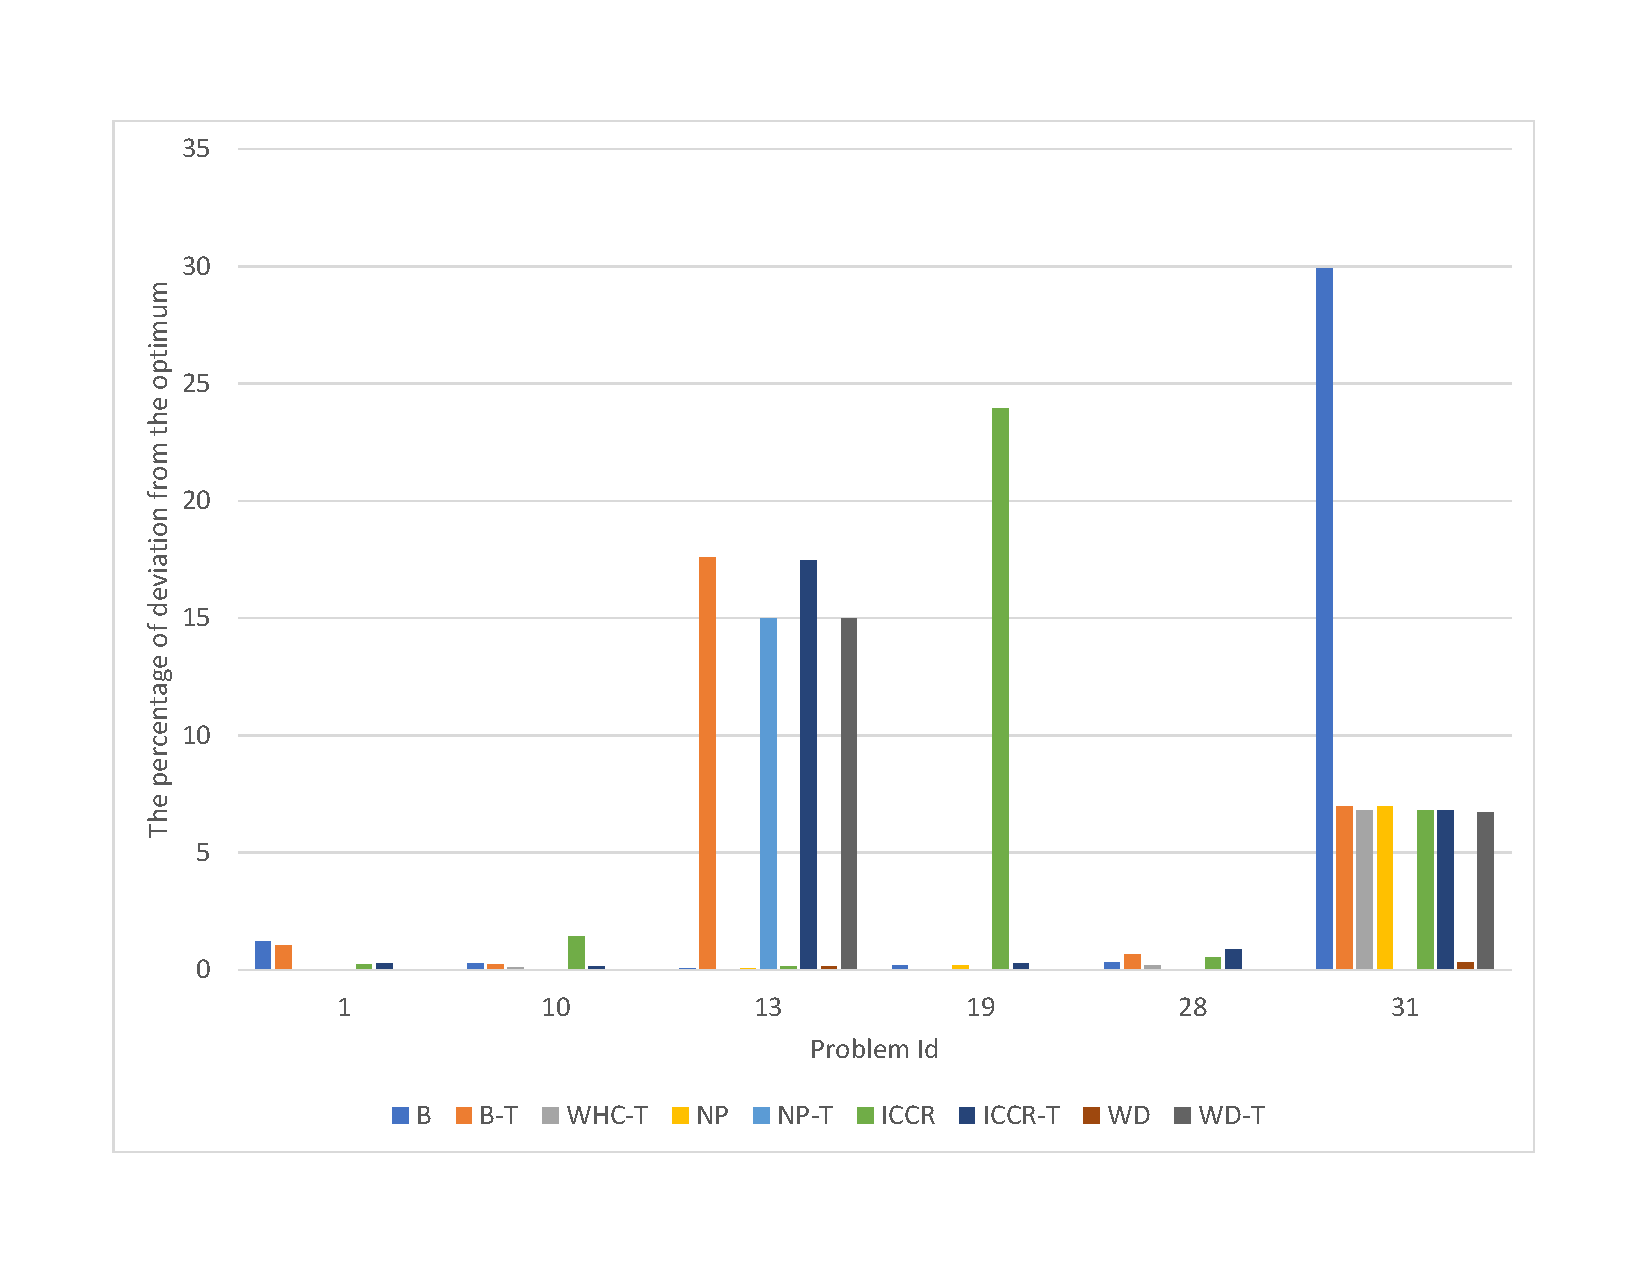
\includegraphics[width=\textwidth]{images/EnergyPercentage.pdf}
	\caption[]{}
	\label{fig:EnergyPercentage}
\end{figure}

Figure~\ref{fig:EnergyPercentage} also shows that the deviation is increasing for big size problems. To confirm that fact, we take two problems with different sizes~(Figures~\ref{fig:SmallMediumProblemEnergy}). These problems solved by all versions of the genetic solver except the B version. Figure~\ref{fig:SmallProblemEnergy} shows the percentage of deviation from optimum for a small size problem. This problem's parameters are:
\begin{itemize}
	\item Software variants: 2,
	\item Number of requests: 2,
	\item Component tree depth: 2,
	\item Resources ratio: 50,
	\item timeout to solve the problem: 5 minutes.
\end{itemize}

The quality of results for the problem is near-optimal because the deviation is less than one percent. The NP-T and WD-T versions give an optimal solution for the problem.

Figure~\ref{fig:MediumProblemEnergy} shows the percentage of deviation from optimum for a bigger size problem. This problem's parameters are:
\begin{itemize}
	\item Software variants: 4,
	\item Number of requests: 1,
	\item Component tree depth: 3,
	\item Resources ratio: 100,
	\item timeout to solve the problem: 5 minutes.
\end{itemize}


The quality of results in a case of the bigger problem is much worse. The minimal deviation is 35\% for the NP-T version because the deviation is less than one percent. The NP-T and WD-T versions give an optimal solution for the problem. The WD and WD-T versions give less number of valid solutions, but with better quality. The quality of the solution from other solvers is lower because the percentage of the deviation is more than 100\%. The reason why the quality of solutions is decreasing with a bigger size of the problem could be a higher number of hardware resources. The higher number of resources means that more hardware resources could satisfy the requirements of the software component. The genetic solver could not find best-suited resources for requested components, and as a result, quality is decreasing. 


\begin{figure}
	\centering
	\begin{subfigure}{0.45\textwidth}
		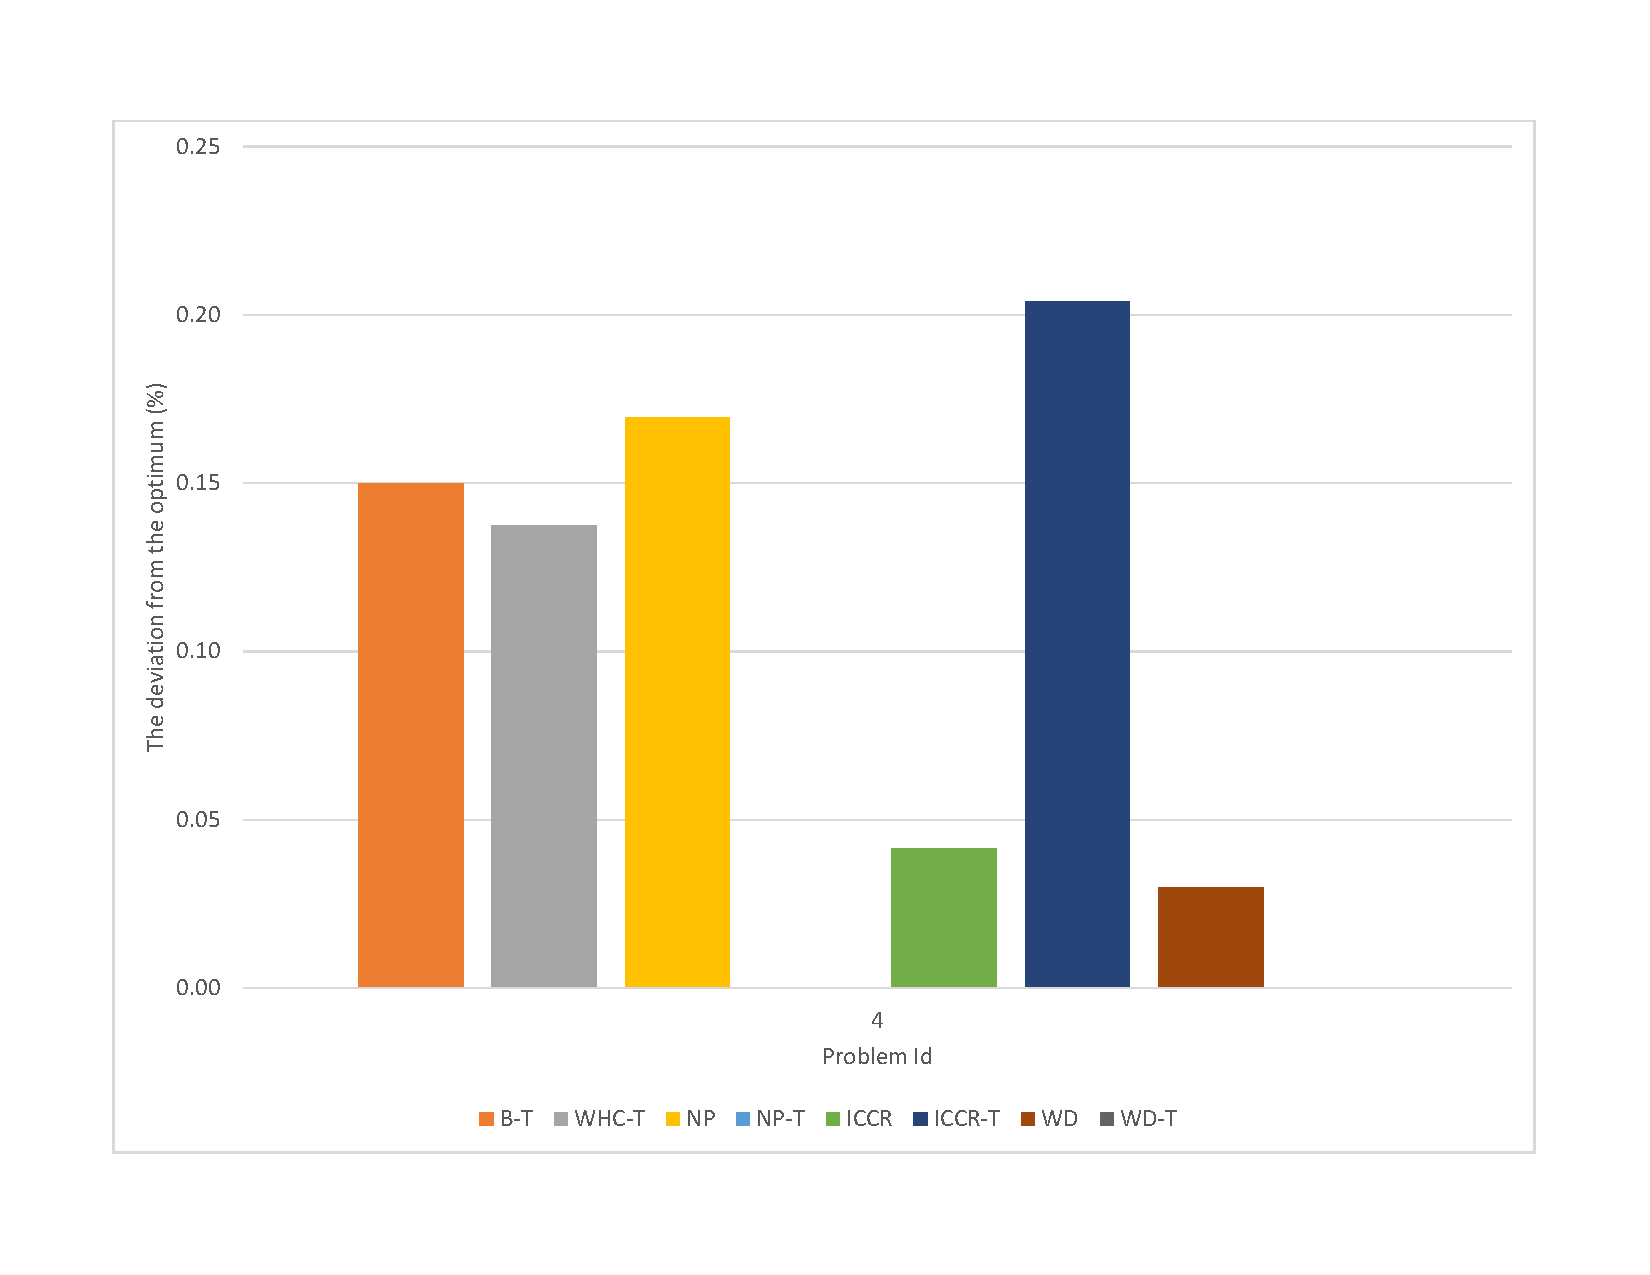
\includegraphics[width=\textwidth]{images/EnergyDeviationSmallProblem.pdf}
		\caption{$y=x$}
		\label{fig:SmallProblemEnergy}
	\end{subfigure}
	\hfill
	\begin{subfigure}{0.45\textwidth}
		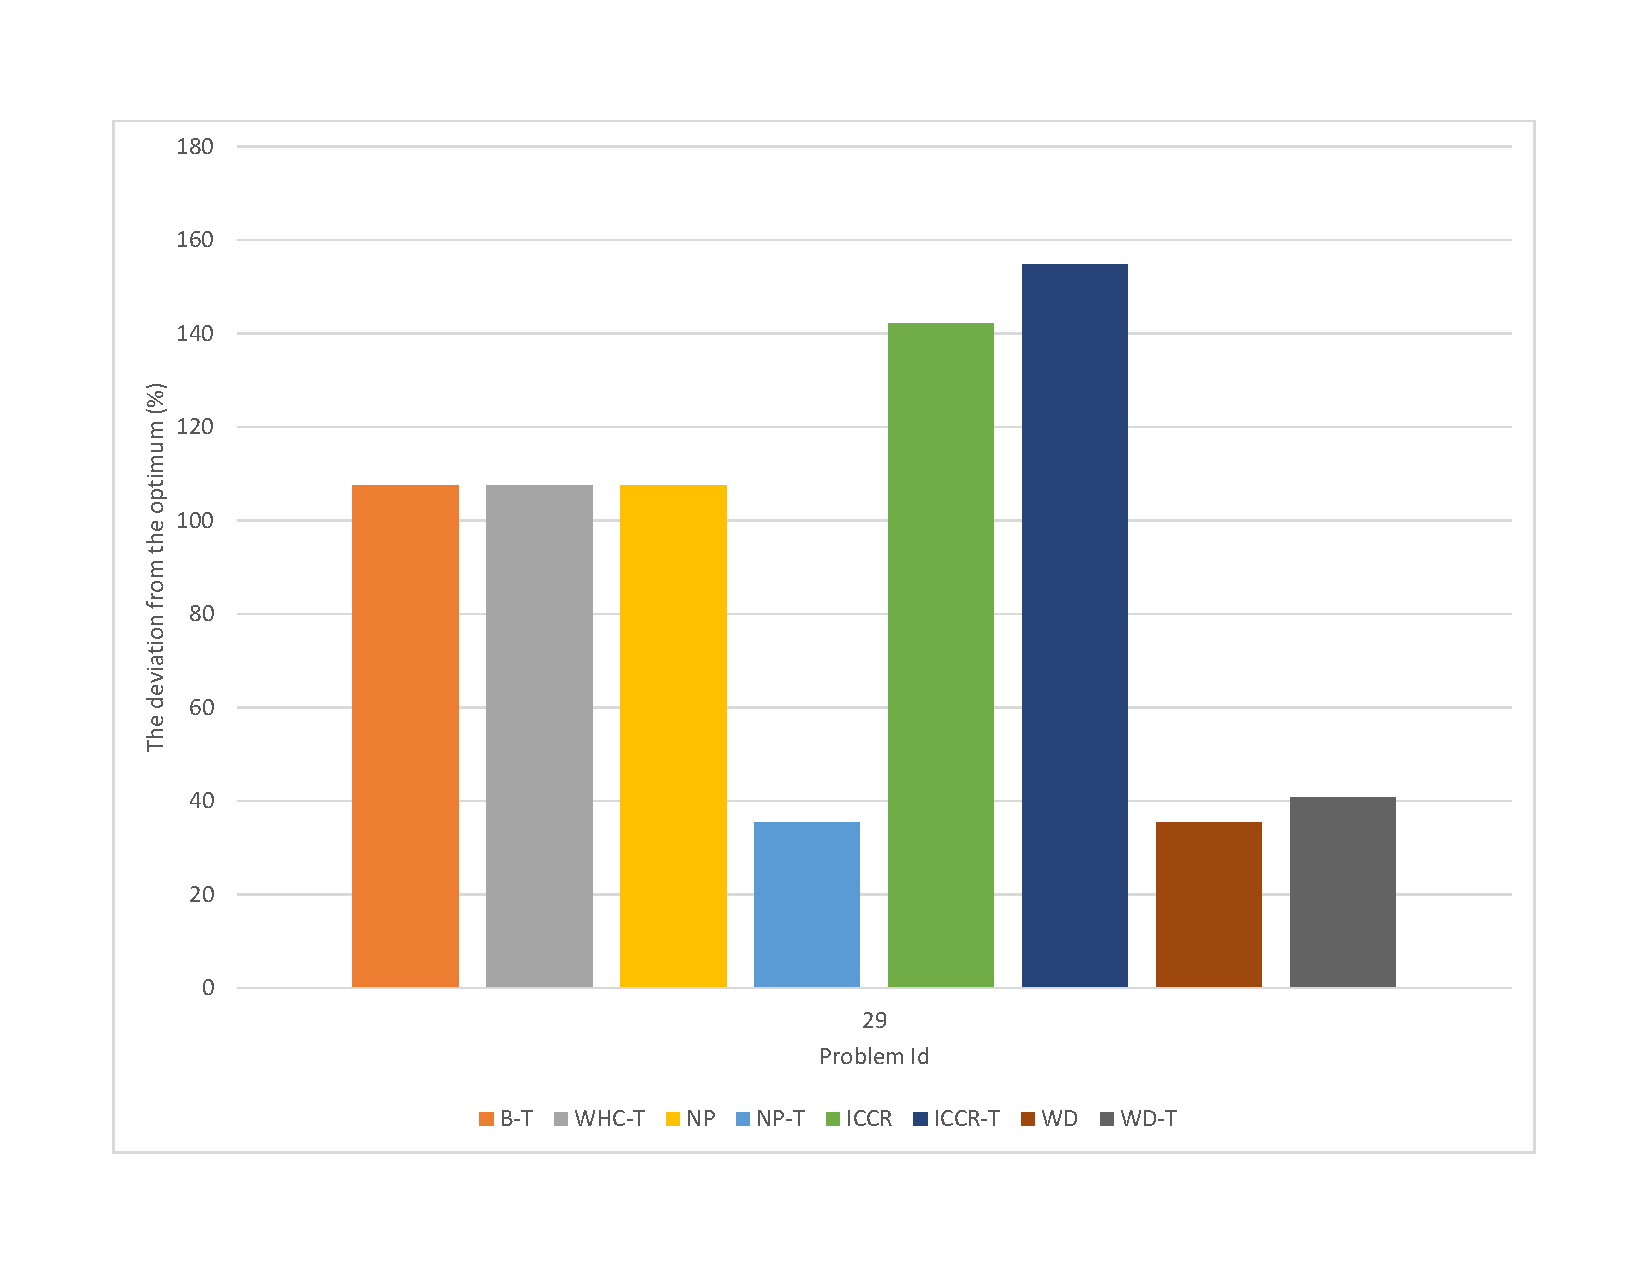
\includegraphics[width=\textwidth]{images/EnergyDeviationMediumProblem.pdf}
		\caption{$y=x$}
		\label{fig:MediumProblemEnergy}
	\end{subfigure}    
	\caption{Three simple graphs}
	\label{fig:SmallMediumProblemEnergy}    
\end{figure}


This section shows that modification that we made improve the results of the genetic solver. The NP-T version solved three times more problems than the B version. We evaluated the quality of solutions. As a result of the quality evaluation, we make two conclusions. First, modified versions of the genetic solver also improve the quality of the results. Second, the quality is decreasing for a bigger size of the problem.
However, there are problems from the set that could not be solved by the genetic solver.


\section{Analysis}

Benchmark showed that a genetic solver could not solve all MQuAT problems from the evaluation set.
In this section, we presented an analysis of results, reasons why described in Chapter~\ref{chapter:Implementation} approaches, and optimizations have lower efficiency that we need.

Firstly, let us discuss the reasons why modifications that we made improve the genetic solver. After that, we will concentrate on the reasons why not all tasks could be solved.

There are a few reasons why the genetic solver with our modifications could solve more problems than the B version. First of all, parameter tuning was performed for all versions. Optimized values of parameters give better results, as it showed in the previous section. The second reason are new probabilities that we added in Section~\ref{sec:NP}. These probabilities give a possibility to change the position of the crossover and mutation points randomly, and as a result, the genetic solver gives results that a bit worse than parameter tuning. 

Nevertheless, not all tasks were solved. One of the reasons for such a result is parameter tuning. We optimized parameters for a specific problem that we described at the beginning of Chapter~\ref{chapter:Implementation}.

Obtained results could be described with a \textbf{"no free lunch" (NFL) theorem}\cite{wolpert1996, wolpert1997}. It says that if an algorithm works well with a certain class of tasks, then it must pay for it with a deterioration in performance on the set of all remaining problems.

Another reason that we optimize parameters without knowledge about dependencies between them. Parameters that we found or added did not fit well for our goals. Let us analyze earlier discussed parameters.

We start an analysis with search space representation. For this representation, we performed measurements for more than three thousand configurations using BRISE in the Search space exploration mode with the NP version of the genetic solver. This mode was described in Section~\ref{sec:BRISE}. For this type of analysis, we use the same problem as in Chapter~\ref{chapter:Implementation} and it has parameter values:
\begin{itemize}
	\item Software variants: 10,
	\item Number of requests: 15,
	\item Component tree depth: 2,
	\item Resources ratio: 5,
	\item timeout to solve the problem: 5 minutes.
\end{itemize}

The search space representation for the SPEA2 selector as a parallel coordinates plot showed in Figure~\ref{fig:SearchSpaceViewFull}.
Each parameter is represented in the plot as a vertical line that contains all possible values of the parameter. Each configuration that was measured showed on the plot as a line that connects all values that describe itself. The last vertical line and the color shows the number of contract violations that give the configuration. The more dark color means fewer contract violations and vise versa, the lighter color gives a higher number of contract violations.

\begin{figure}
	\centering
	\includegraphics[width=\textwidth]{images/SPEA2.pdf}
	\caption[]]{}
	\label{fig:SearchSpaceViewFull}
\end{figure}

Figure~\ref{fig:SearchSpaceViewFull} shows all values of parameters could give "good" and "bad" results. There are no visible dependencies between parameters. 

\begin{figure}
	\centering
	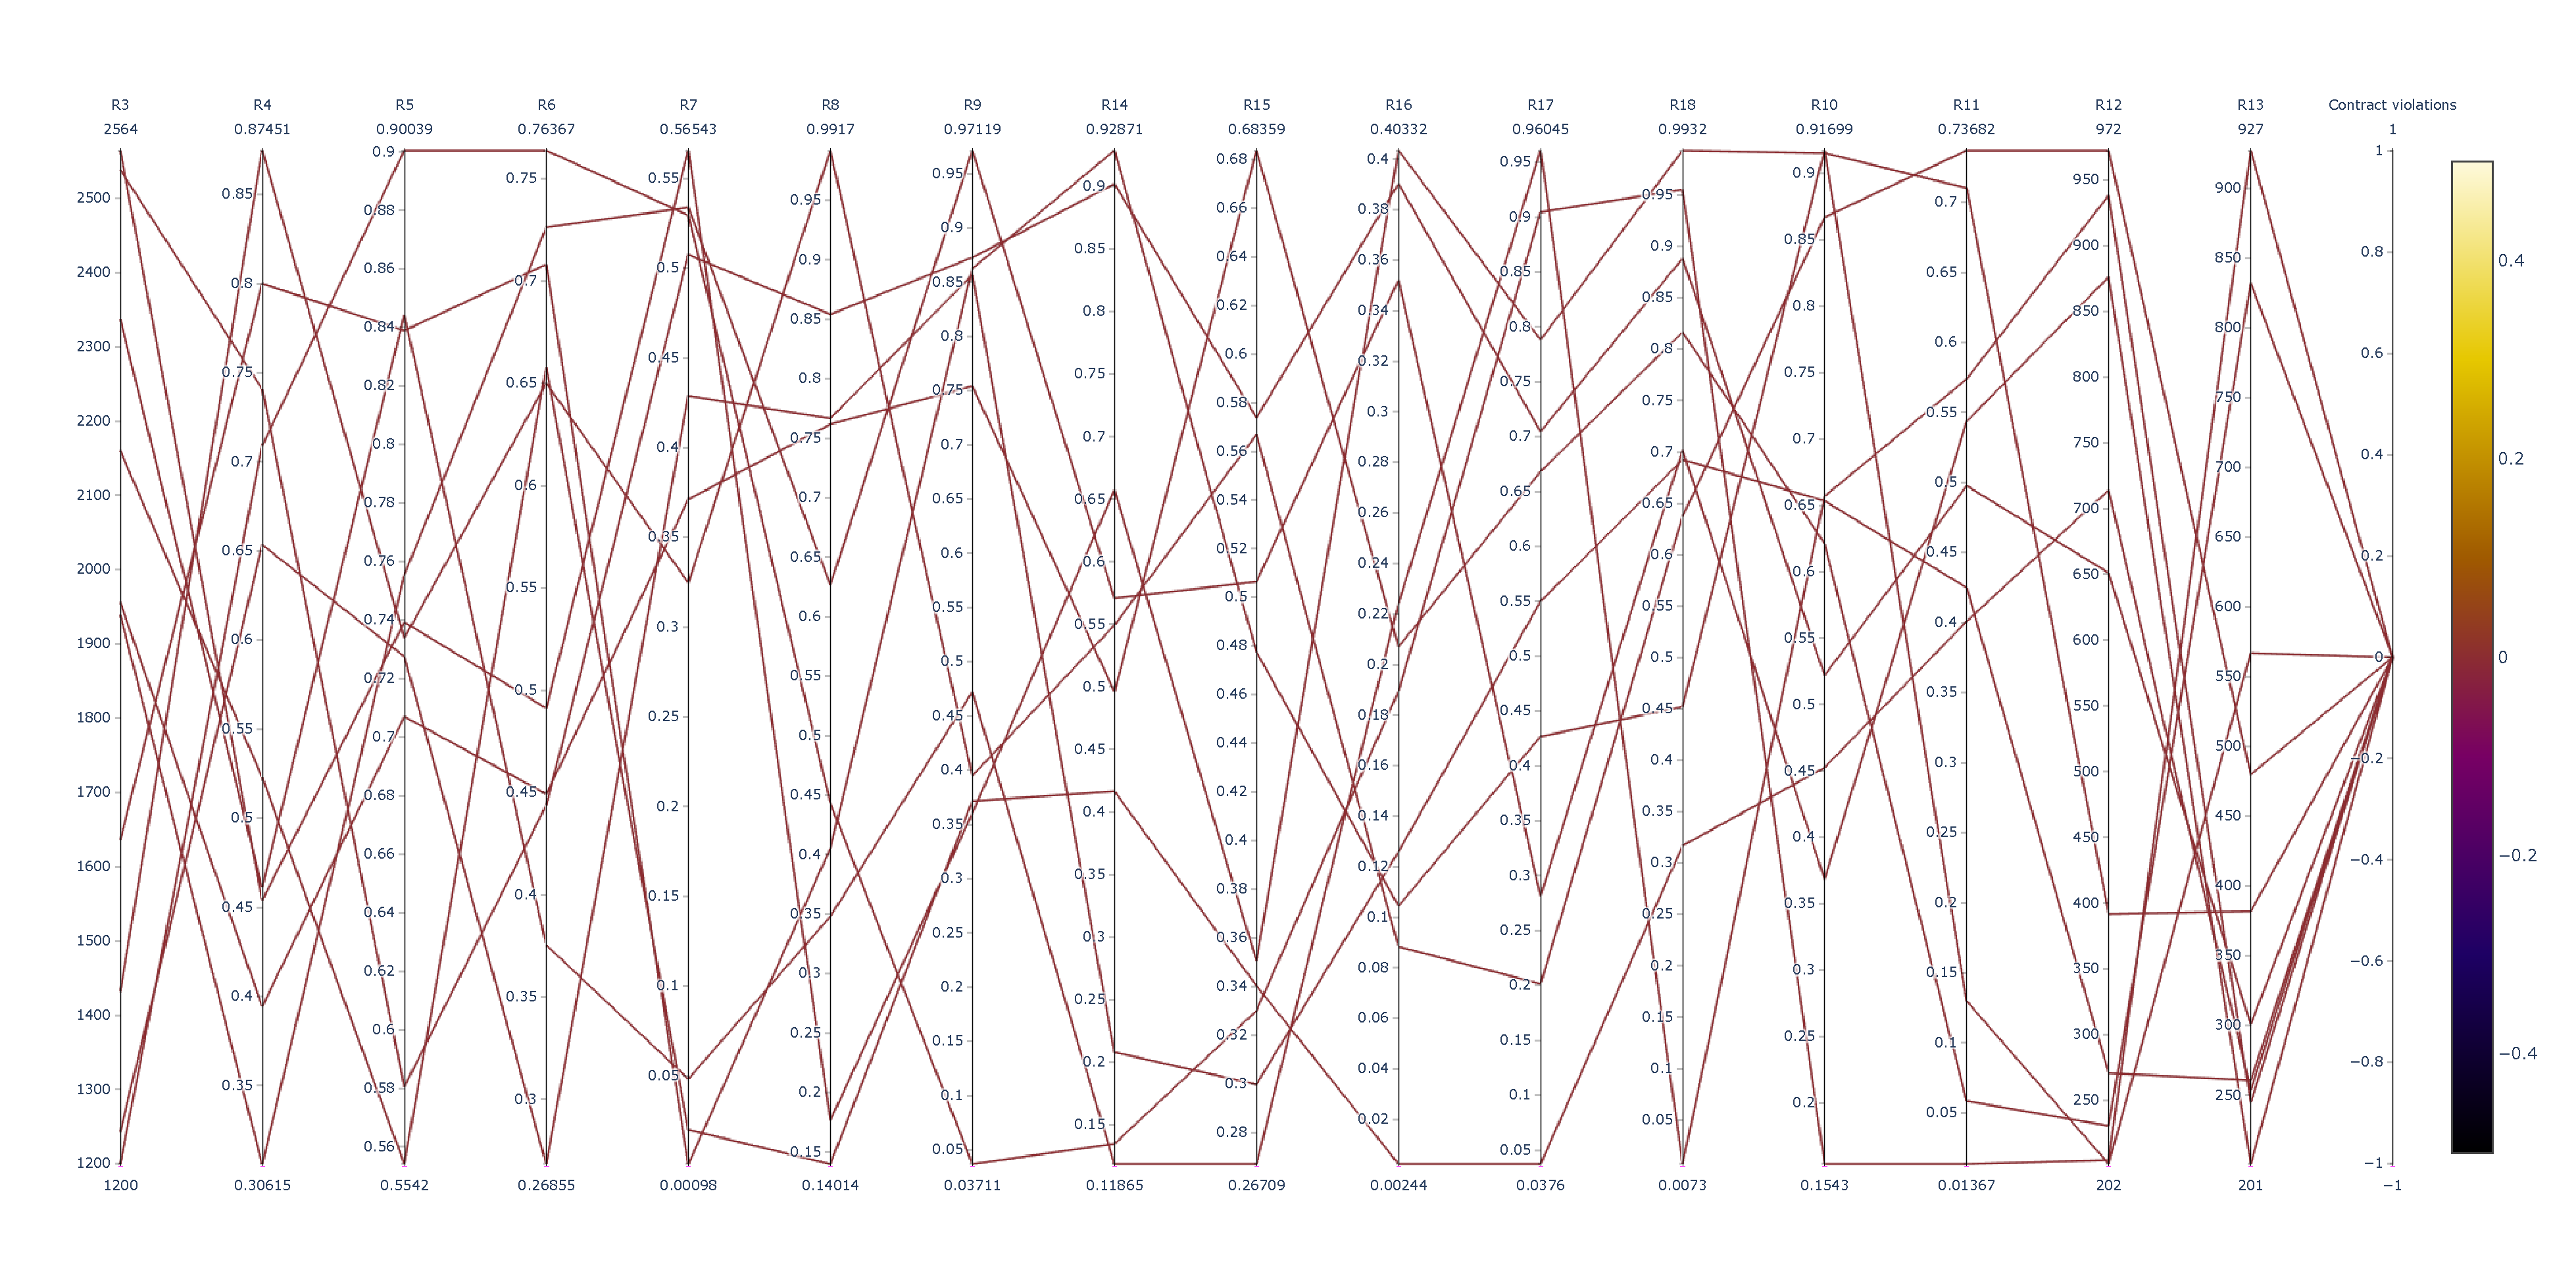
\includegraphics[width=\textwidth]{images/SPEA2_Zero_validity.html.pdf}
	\caption[]]{}
	\label{fig:SearchSpaceValid}
\end{figure}

If we are filtering out all configurations that gave not valid results, we obtained the search space with a few configurations that give valid results. A parallel plot that demonstrates this situation showed in Figure~\ref{fig:SearchSpaceValid}. The plot shows that only a few configurations give a valid result for the specified problem. However, still, there are no visible dependencies between the parameters and the number of contract violations, or between the parameters themselves.

\begin{figure}
	\centering
	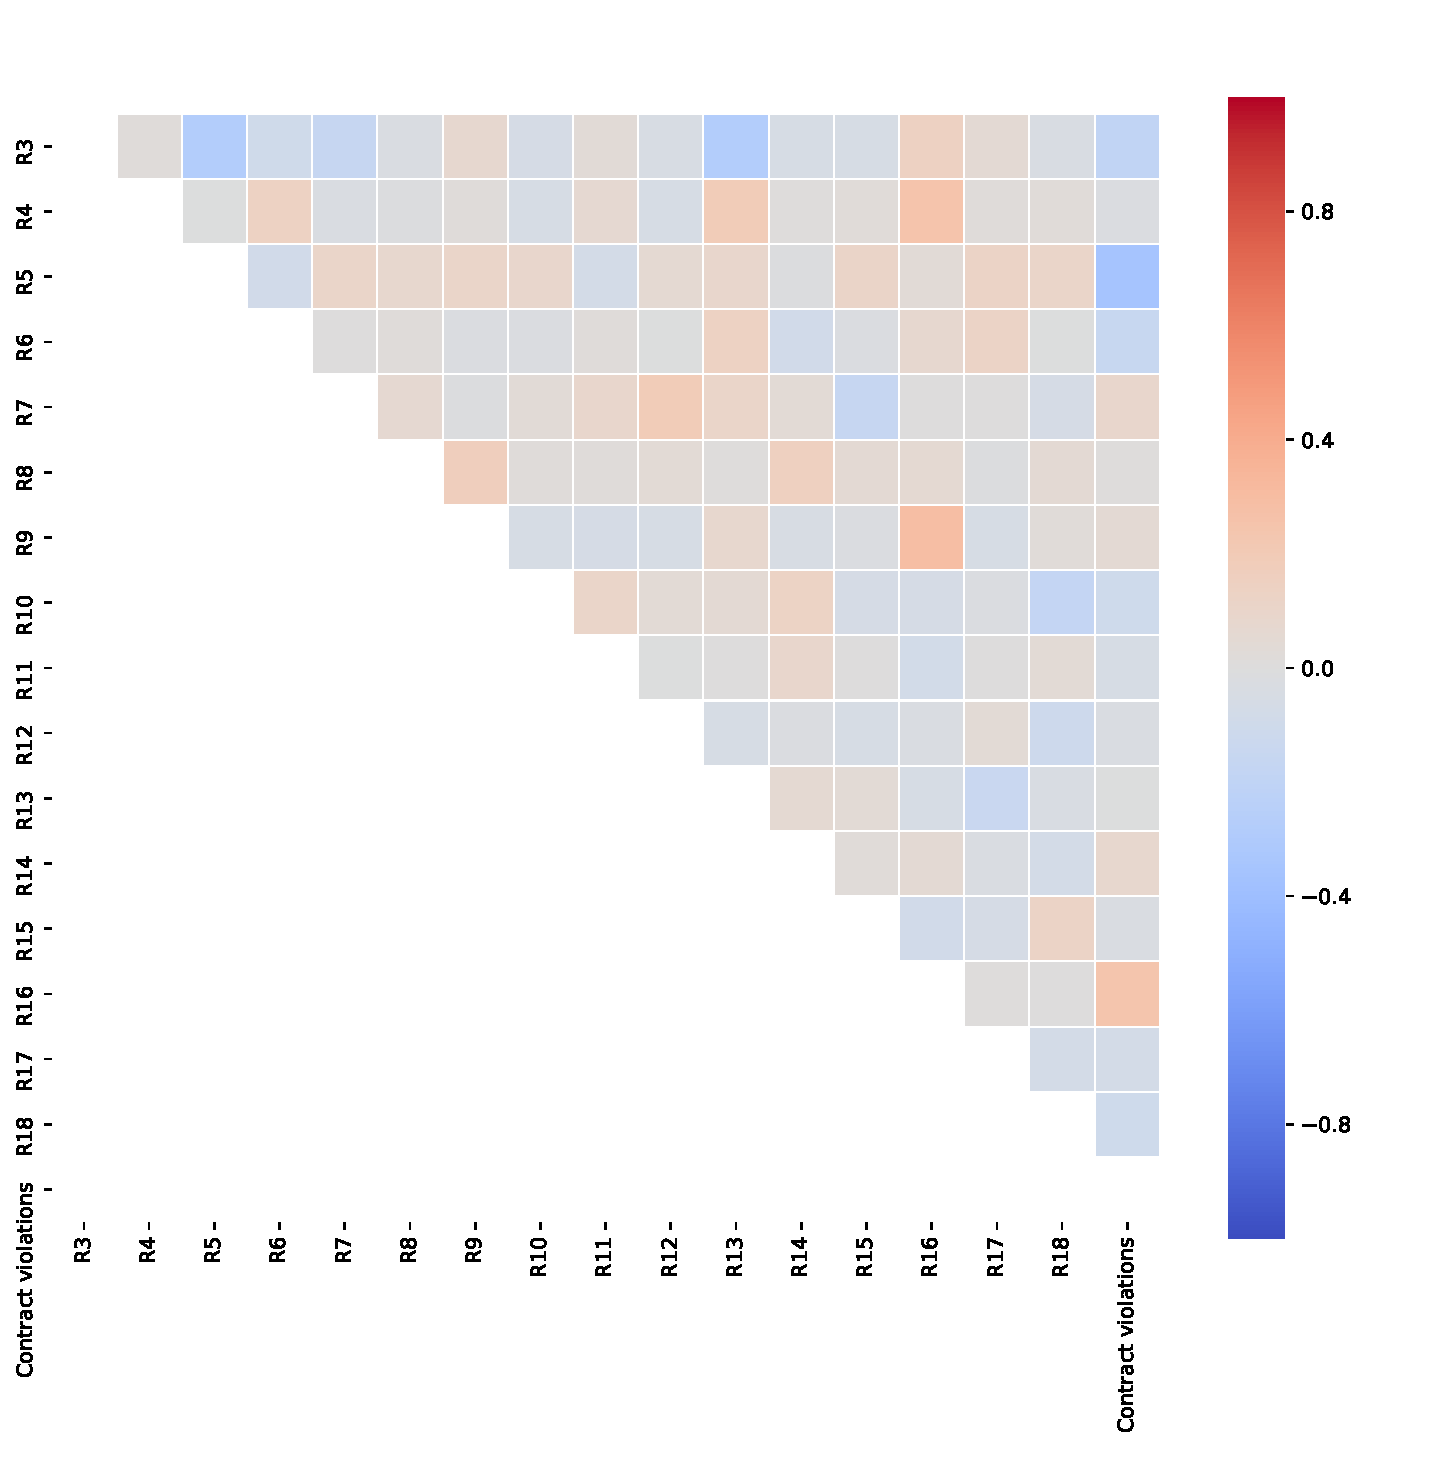
\includegraphics[width=\textwidth]{images/CorrelationAnalysis.pdf}
	\caption[]]{}
	\label{fig:CorrelationAnalysis}
\end{figure}

Cause Figure~\ref{fig:SearchSpaceViewFull} and Figure~\ref{fig:SearchSpaceValid} show that the search space view could not give any conclusions about dependencies between parameters or between parameters and number of contract violations, another method of analysis was performed.

We performed the correlation analysis of parameters to understand how are they relay on each other. The results showed in Figure~\ref{fig:CorrelationAnalysis} as a correlation matrix where the value of the correlation is the color of the cell. Each row and column in this matrix represent the parameter of the genetic algorithm. There is only an upper triangle of the matrix because it is symmetric. The last column of the matrix represents the correlation between parameters of the genetic solver (NP version) and a number of contract violations~(CVs). There are two types of correlation. Direct correlation showed with red color and an inverse correlation with blue color. In the case of the last column, direct correlation means that a bigger value o parameter gives a bigger number of contract violations. Inverse correlation, in the same case, means that the bigger value of parameter gives a smaller number of contract violations. Grey color shows that there is no correlation between values.

From the correlation analysis, we can conclude that there are no strong dependencies between the number of contract violations and parameters. There are two more important parameters: \texttt{CrossoverRate}(R5) and \texttt{CrossoverOnRandomRequestProbability}(R16).
The analysis showed that the \texttt{CrossoverRate} parameter needs to have big value and value of \texttt{CrossoverOnRandomRequestProbability} needs to be as low as possible. In this case of the small value of probability, it may be a good idea to remove this parameter for parameter tuning.

Correlation analysis showed that some parameters have dependencies. Nevertheless, we do not know yet how they depend.

For further investigation of dependencies, we constructed plots that show the distribution of parameter pairs. We will discuss only two distribution. The first plot will show one representative distribution, and the second plot represents how most of the constructed distributions look like.

\begin{figure}
	\centering
	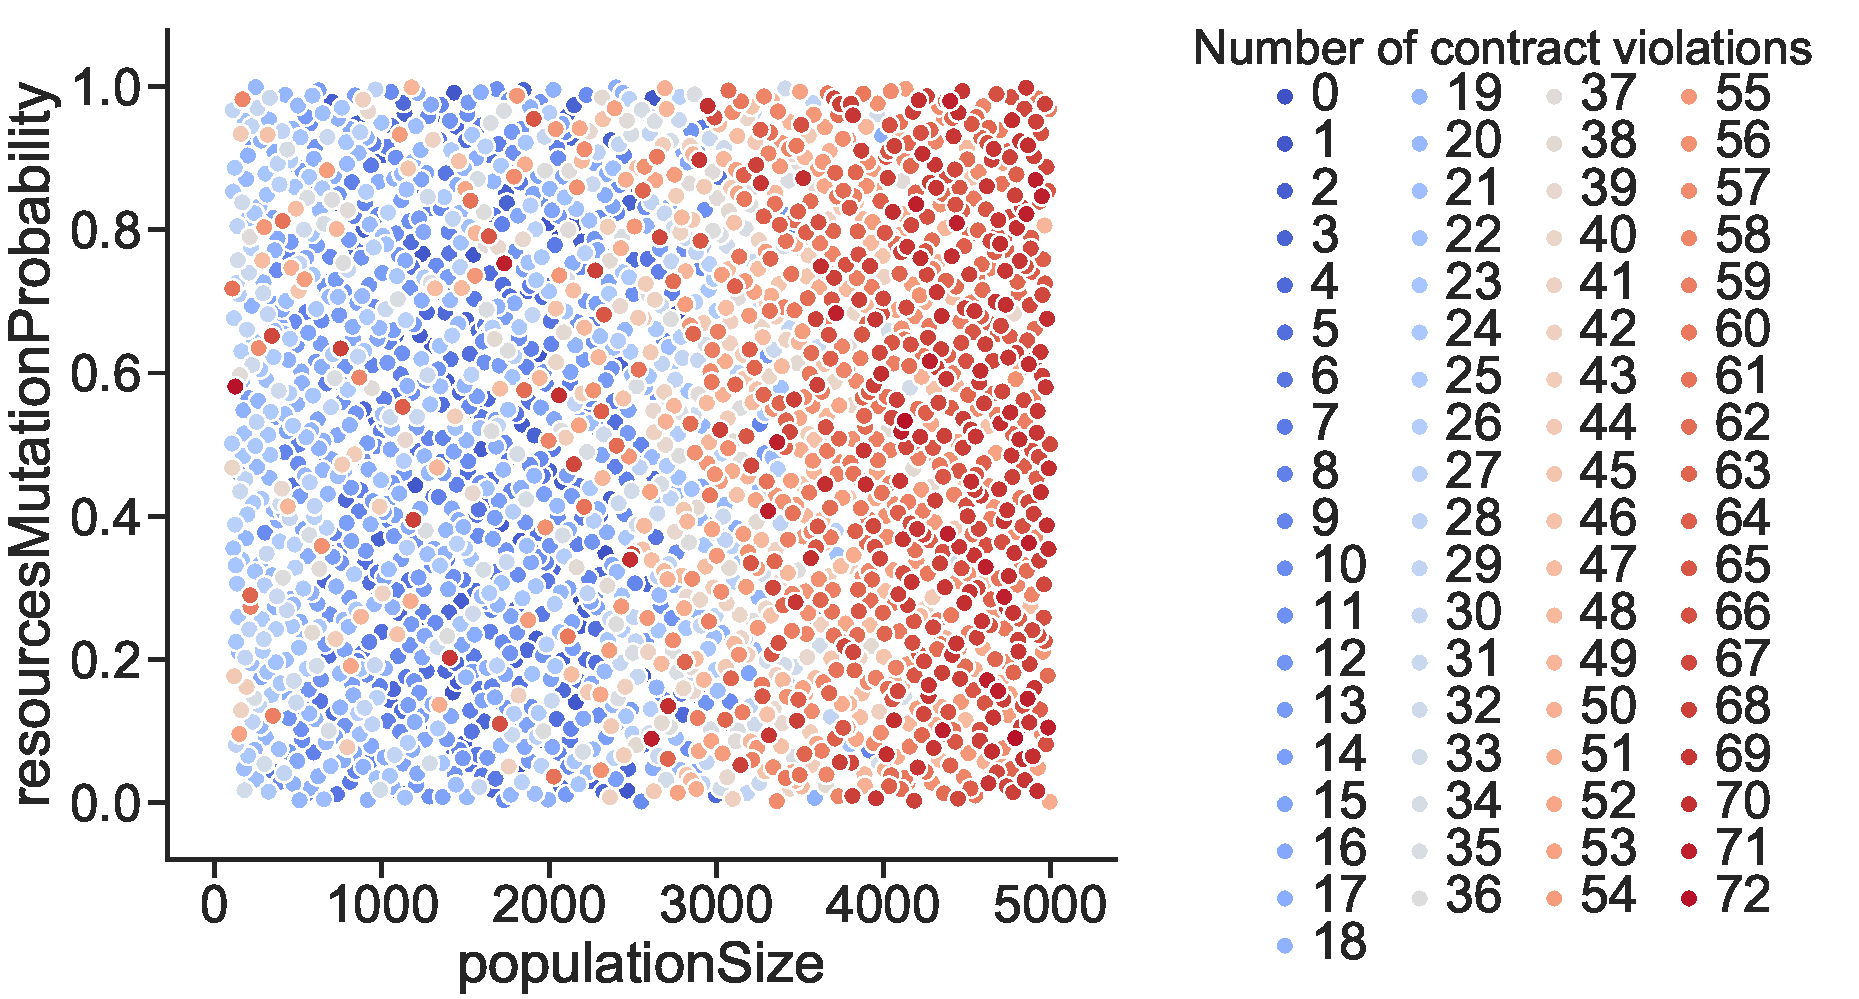
\includegraphics[width=\textwidth]{images/populatioSizeVsResMutationProbability.pdf}
	\caption[]]{}
	\label{fig:populatioSizeVsResMutationProbability}
\end{figure}

The representative distribution showed in Figure~\ref{fig:populatioSizeVsResMutationProbability}. Each point on this plot represent a value combination of two parameters \texttt{populationSize}~(R3) and \texttt{resourcesMutationProbability}~(R8). The color of the point is the number of contract violations. In this case, blue color is a small number of contract violations. Red color represents a big number of contract violations. As we can see, there is gradient coloring from the mostly blue on the left size to mostly red on the right size. Such result means that \texttt{populationSize}~(R3) have a bigger influence on the result than \texttt{resourcesMutationProbability}~(R8). The figure also shows that for any value of \texttt{resourcesMutationProbability}~(R8), there are results with any number of contract violations.

\begin{figure}
	\centering
	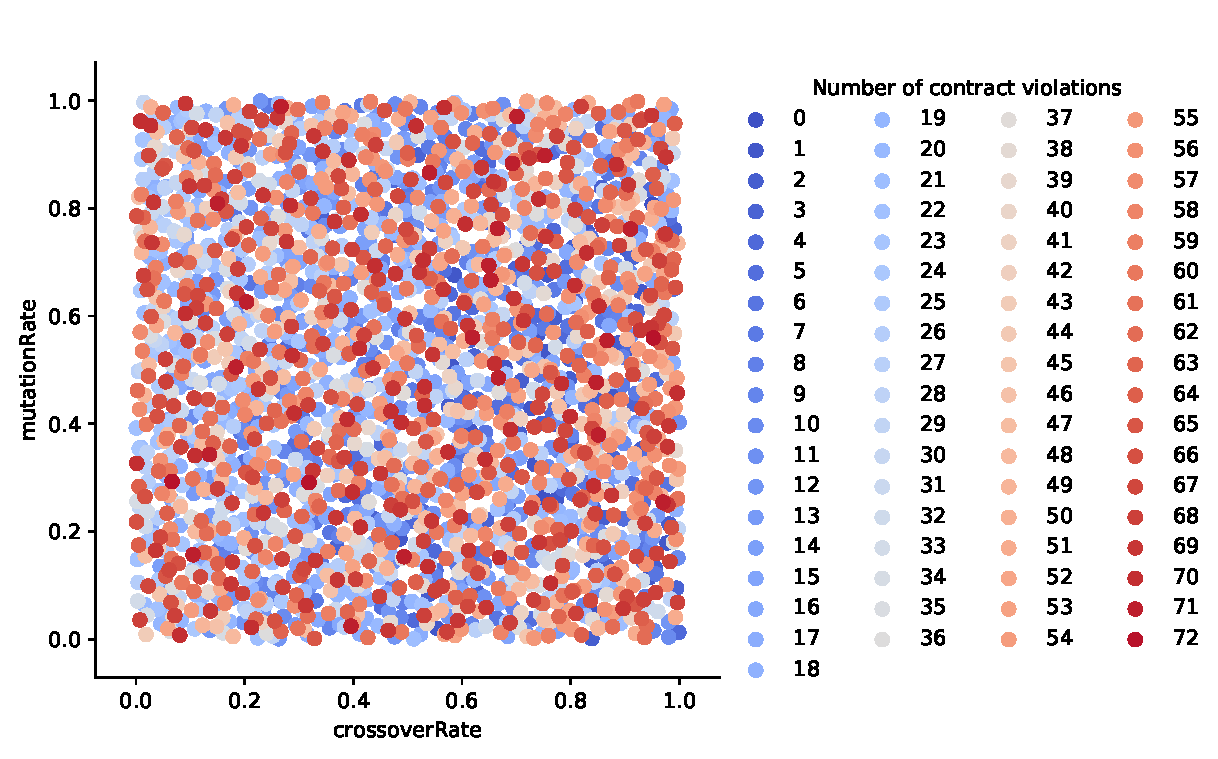
\includegraphics[width=\textwidth]{images/CrossoverRateVsutationRate.pdf}
	\caption[]]{}
	\label{fig:CrossoverRateVmutationRate}
\end{figure}

However, most distributions look like the distribution of \texttt{crossoverRate}~(R5) and \texttt{mutationRate}~(R7). It showed in Figure~\ref{fig:CrossoverRateVsutationRate}. As we can see, "good" and "bad" results exist for all values of the described parameters. That means that these parameters do not depend on each other.

Distributions of combinations of two parameters showed that some parameters have a more significant impact on the result than others. Moreover, there are parameters on the value of which the result does not depend. More examples of such distributions showed in Appendix~\ref{label}.

\begin{figure}
	\subfloat[Name A]{%
		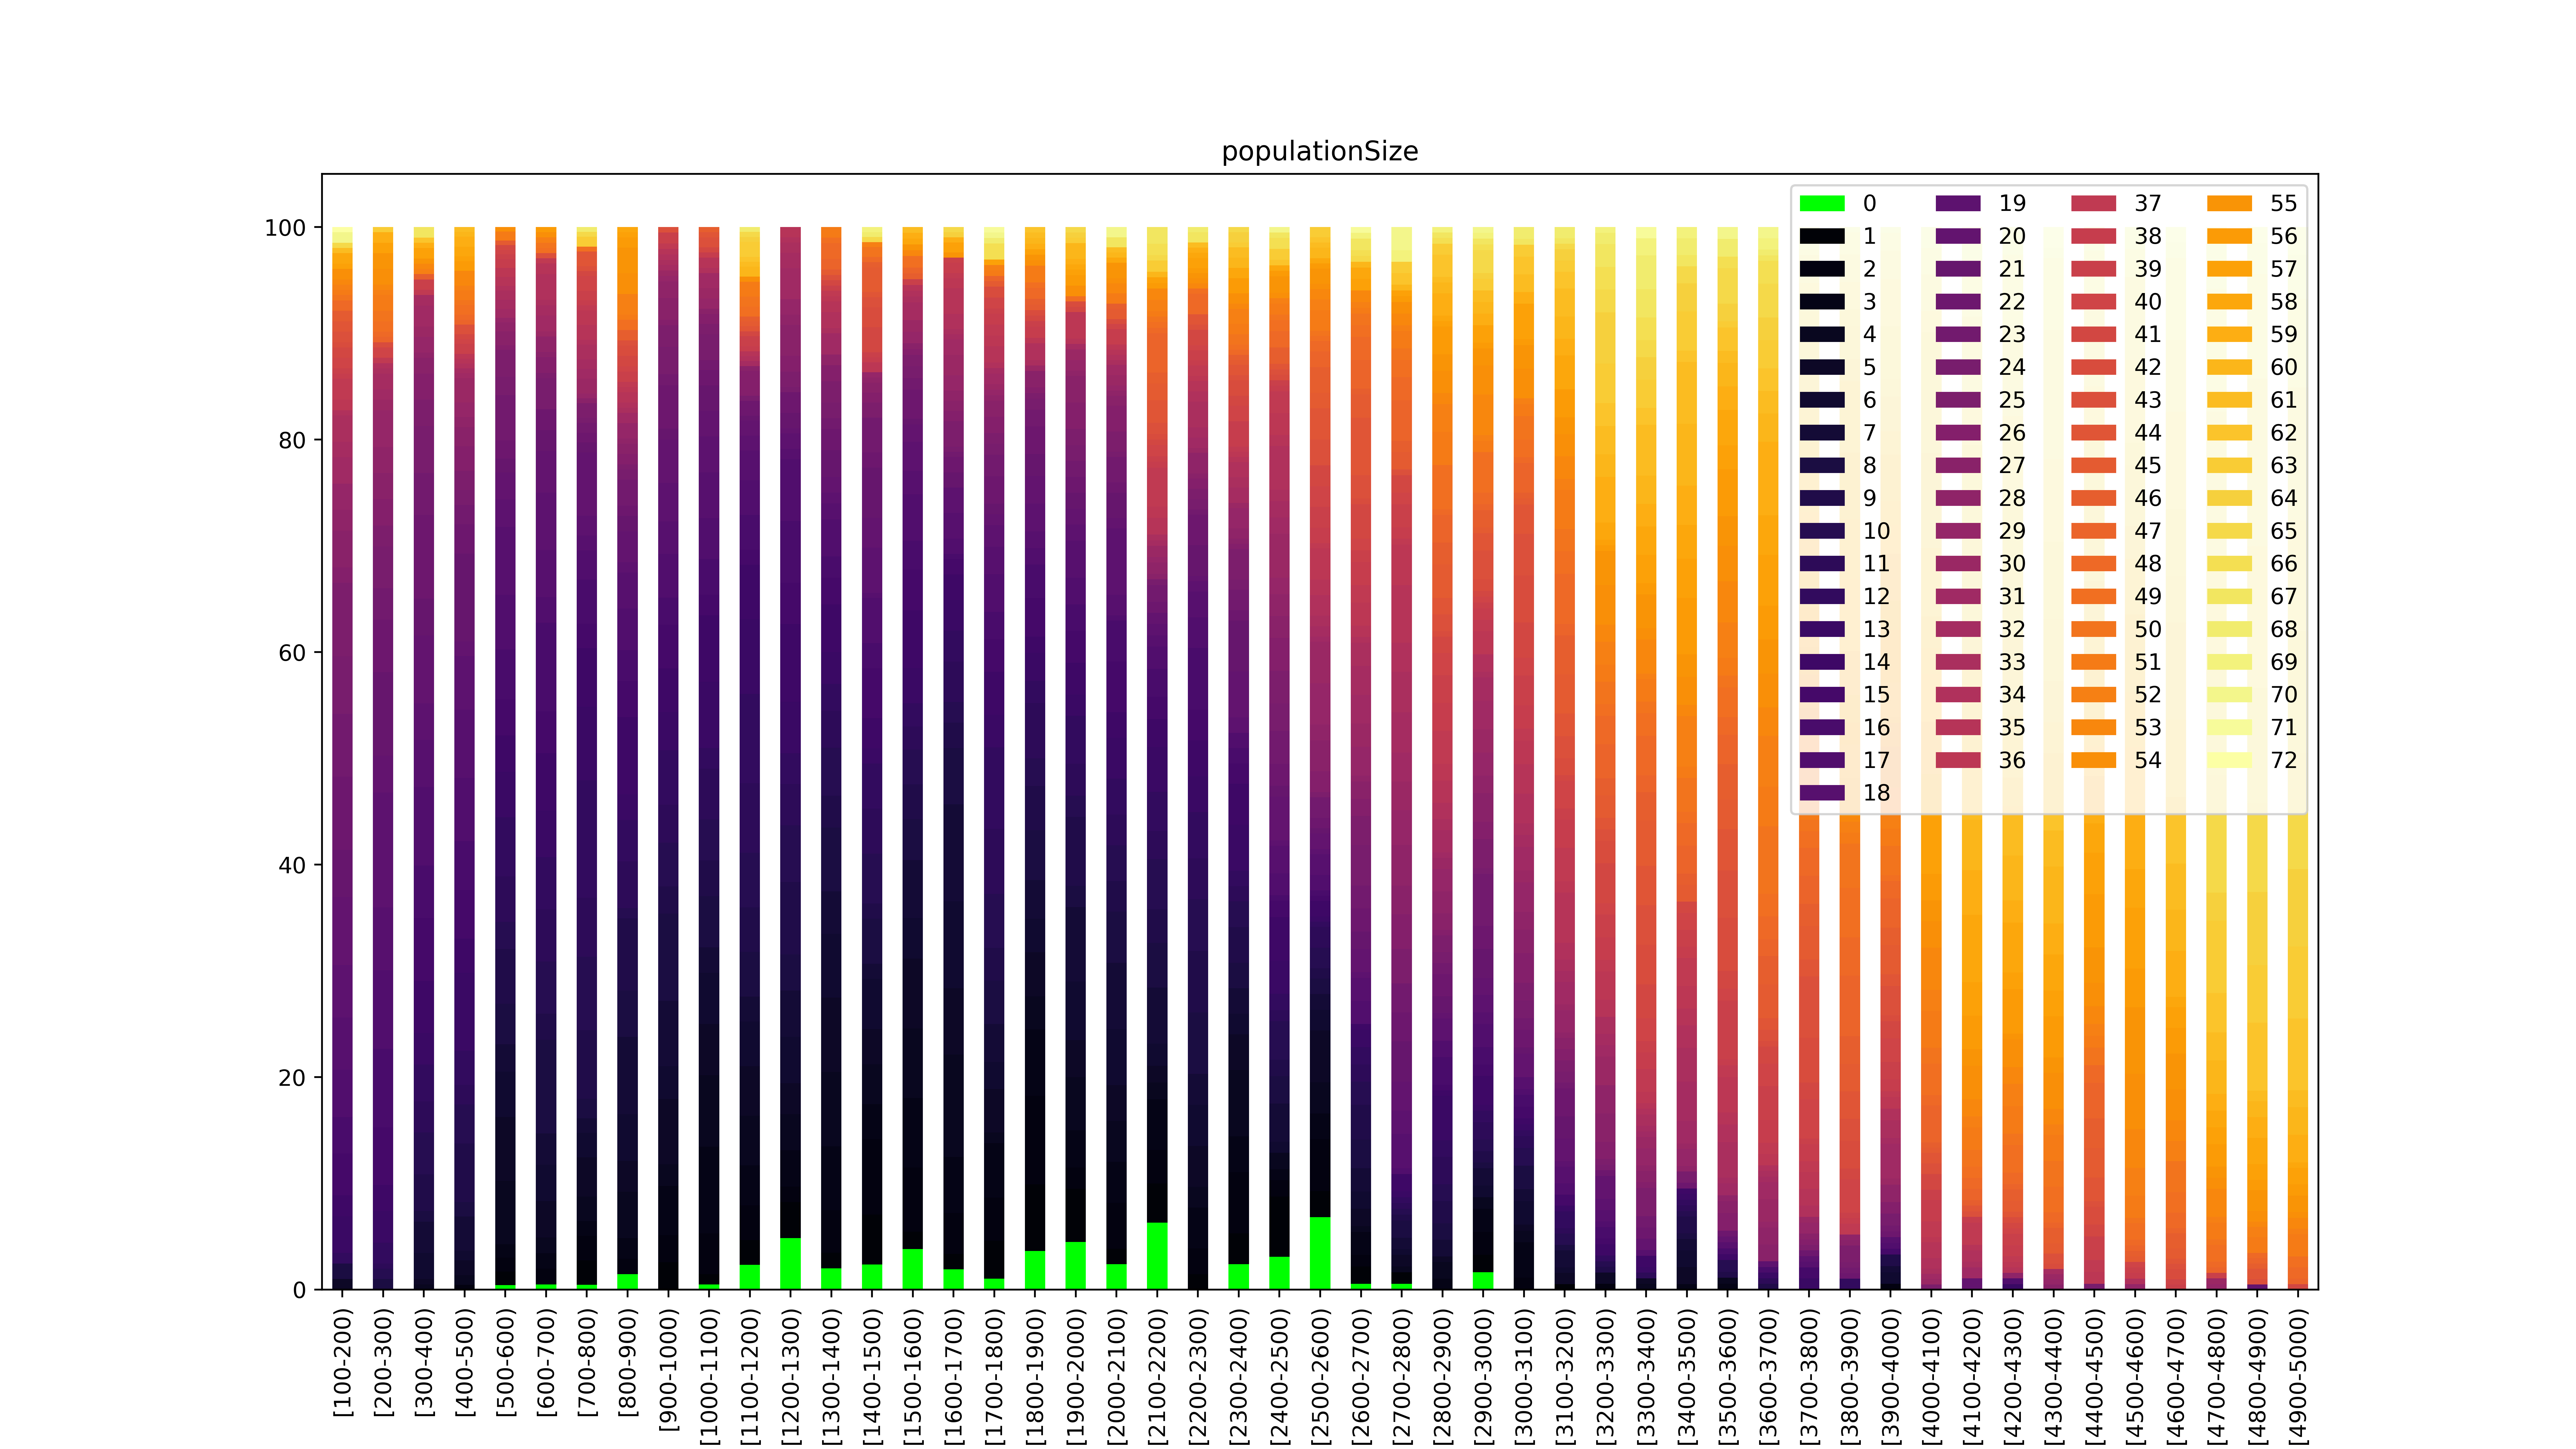
\includegraphics[clip,width=\textwidth]{images/populationSize_gradientBig.png}%
		\label{fig:populationSize_gradientBig}
	}
	
	\subfloat[Name b]{%
		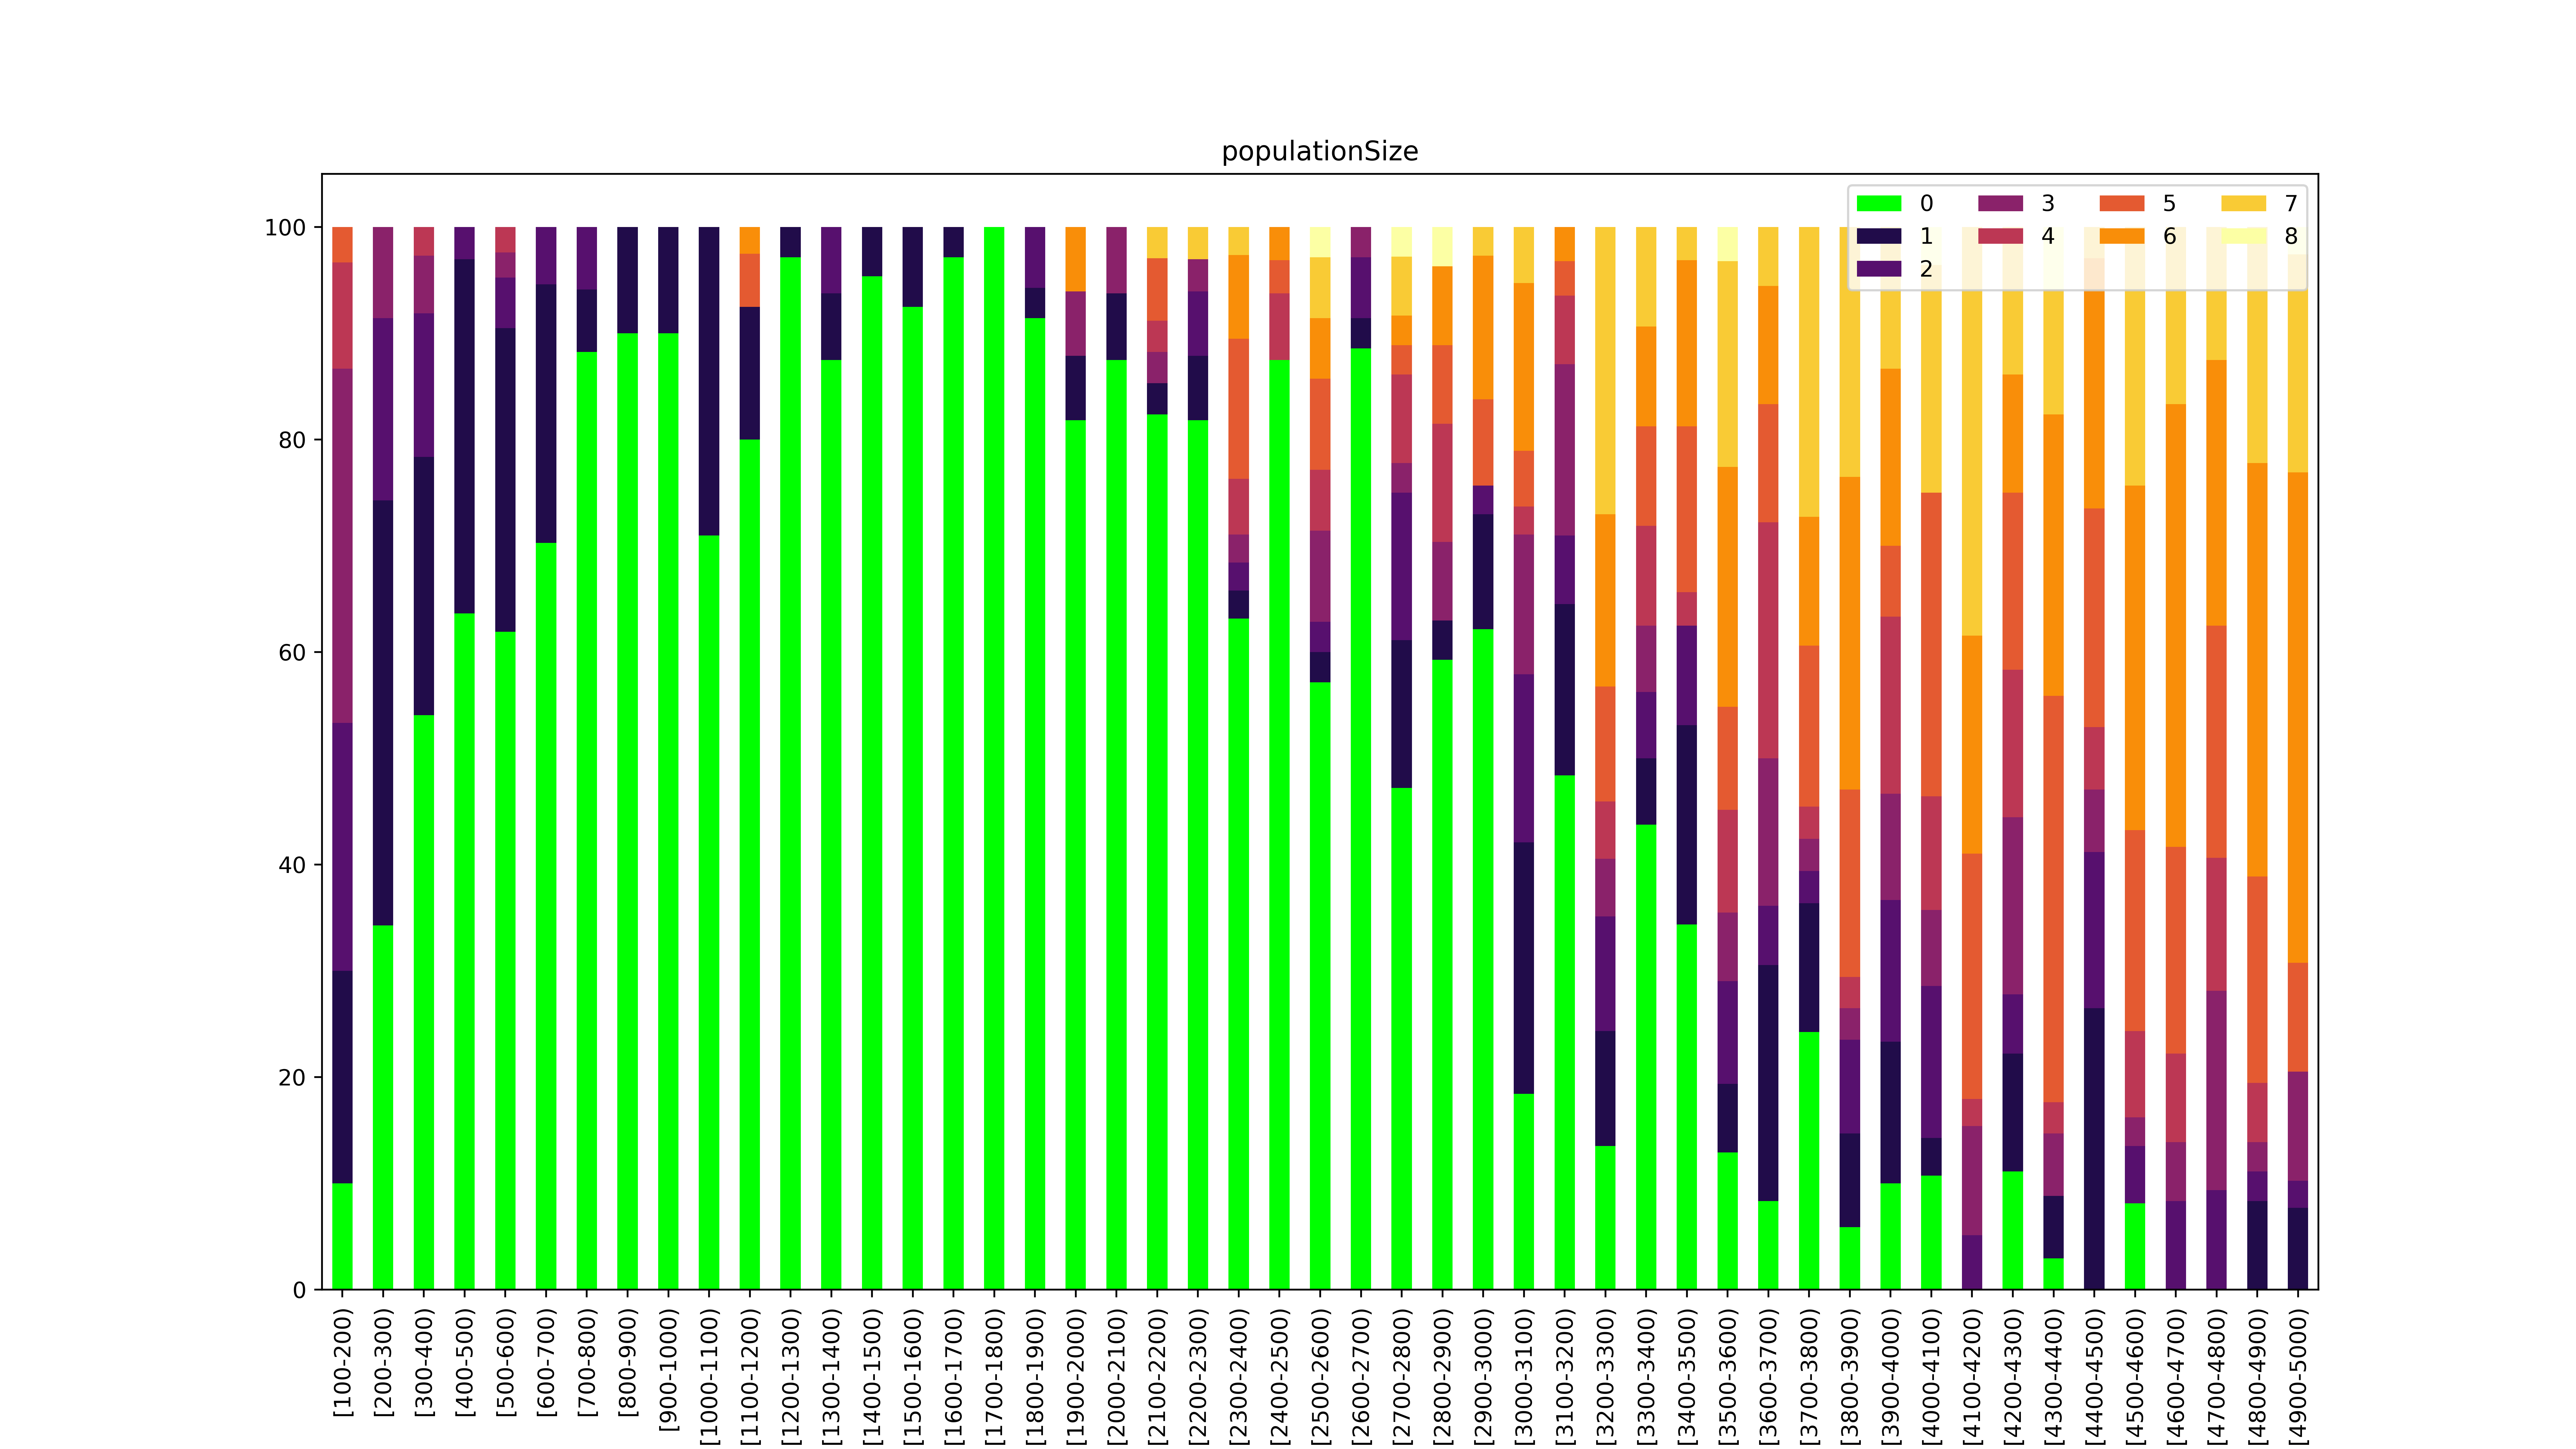
\includegraphics[clip,width=\textwidth]{images/populationSize_gradientSmall.png}%
		\label{fig:populationSize_gradientSmall}
	}
	
	\caption{main caption}
	\label{fig:populationSize_gradient}
\end{figure}

Previously discussed plots show that the results of the genetic solver depend on some parameters such as \texttt{populationSize}~(R3). So we need to analyze how the value of this parameter affects the result. Firstly we discuss the \texttt{populationSize}~(R3) parameter and the second parameter is \texttt{mutationRate}~(R7).

Figure~\ref{fig:populationSize_gradientBig} shows the distribution of the \texttt{populationSize}~(R3) parameter values and the number of contract violations that this value could give. The X-axis is a set of ranges of values for the parameter \texttt{populationSize}~(R3). Each range consists of 100 values. All ranges are sorted. A normalized bar is built for each range. Each bar consists of segments of different heights and colors. The segment color shows the number of contract violations, where black is one violation, and yellow is a large number of violations. The green color of the segment indicates valid results(zero contract violations). The segment height of one color means a percentage of the total number of configurations that have the same parameter value and which give the result with the same number of contact failures.

This distribution shows that the left side and the central part of the plot give a smaller number of contract violations because sectors have mainly dark colors and green color. The right side of the distribution contains higher values of the parameter. Moreover, solutions with those values give more contract violations. As can be seen, valid solutions located in the range from 1000 to 2600.

For a more visual image, we construct a similar graph for the smaller problem. This problem described with parameters:
\begin{itemize}
	\item Software variants: 2,
	\item Number of requests: 2,
	\item Component tree depth: 2,
	\item Resources ratio: 5,
	\item timeout to solve the problem: 5 minutes.
\end{itemize}

It is shown in Figure~\ref{fig:populationSize_gradientSmall}. If we compare Figure~\ref{fig:populationSize_gradientSmall} and Figure~\ref{fig:populationSize_gradientBig}, we can see that they have a similar distribution.

The second  discussed parameter is \texttt{mutationRate}~(R7). The distribution of values of this parameter showed in Figure~\ref{fig:mutationRate_gradient}. For better visual understanding, the distribution is built for a smaller problem described above. 
As we can see, the percentage of valid results for any described range of values of the \texttt{mutationRate}~(R7) parameter varies from 50 to 60. The distributions of most parameters look like the distribution described here. Such a distribution means that the result of the genetic solver does not depend on the value of the parameter. 

\begin{figure}
	\centering
	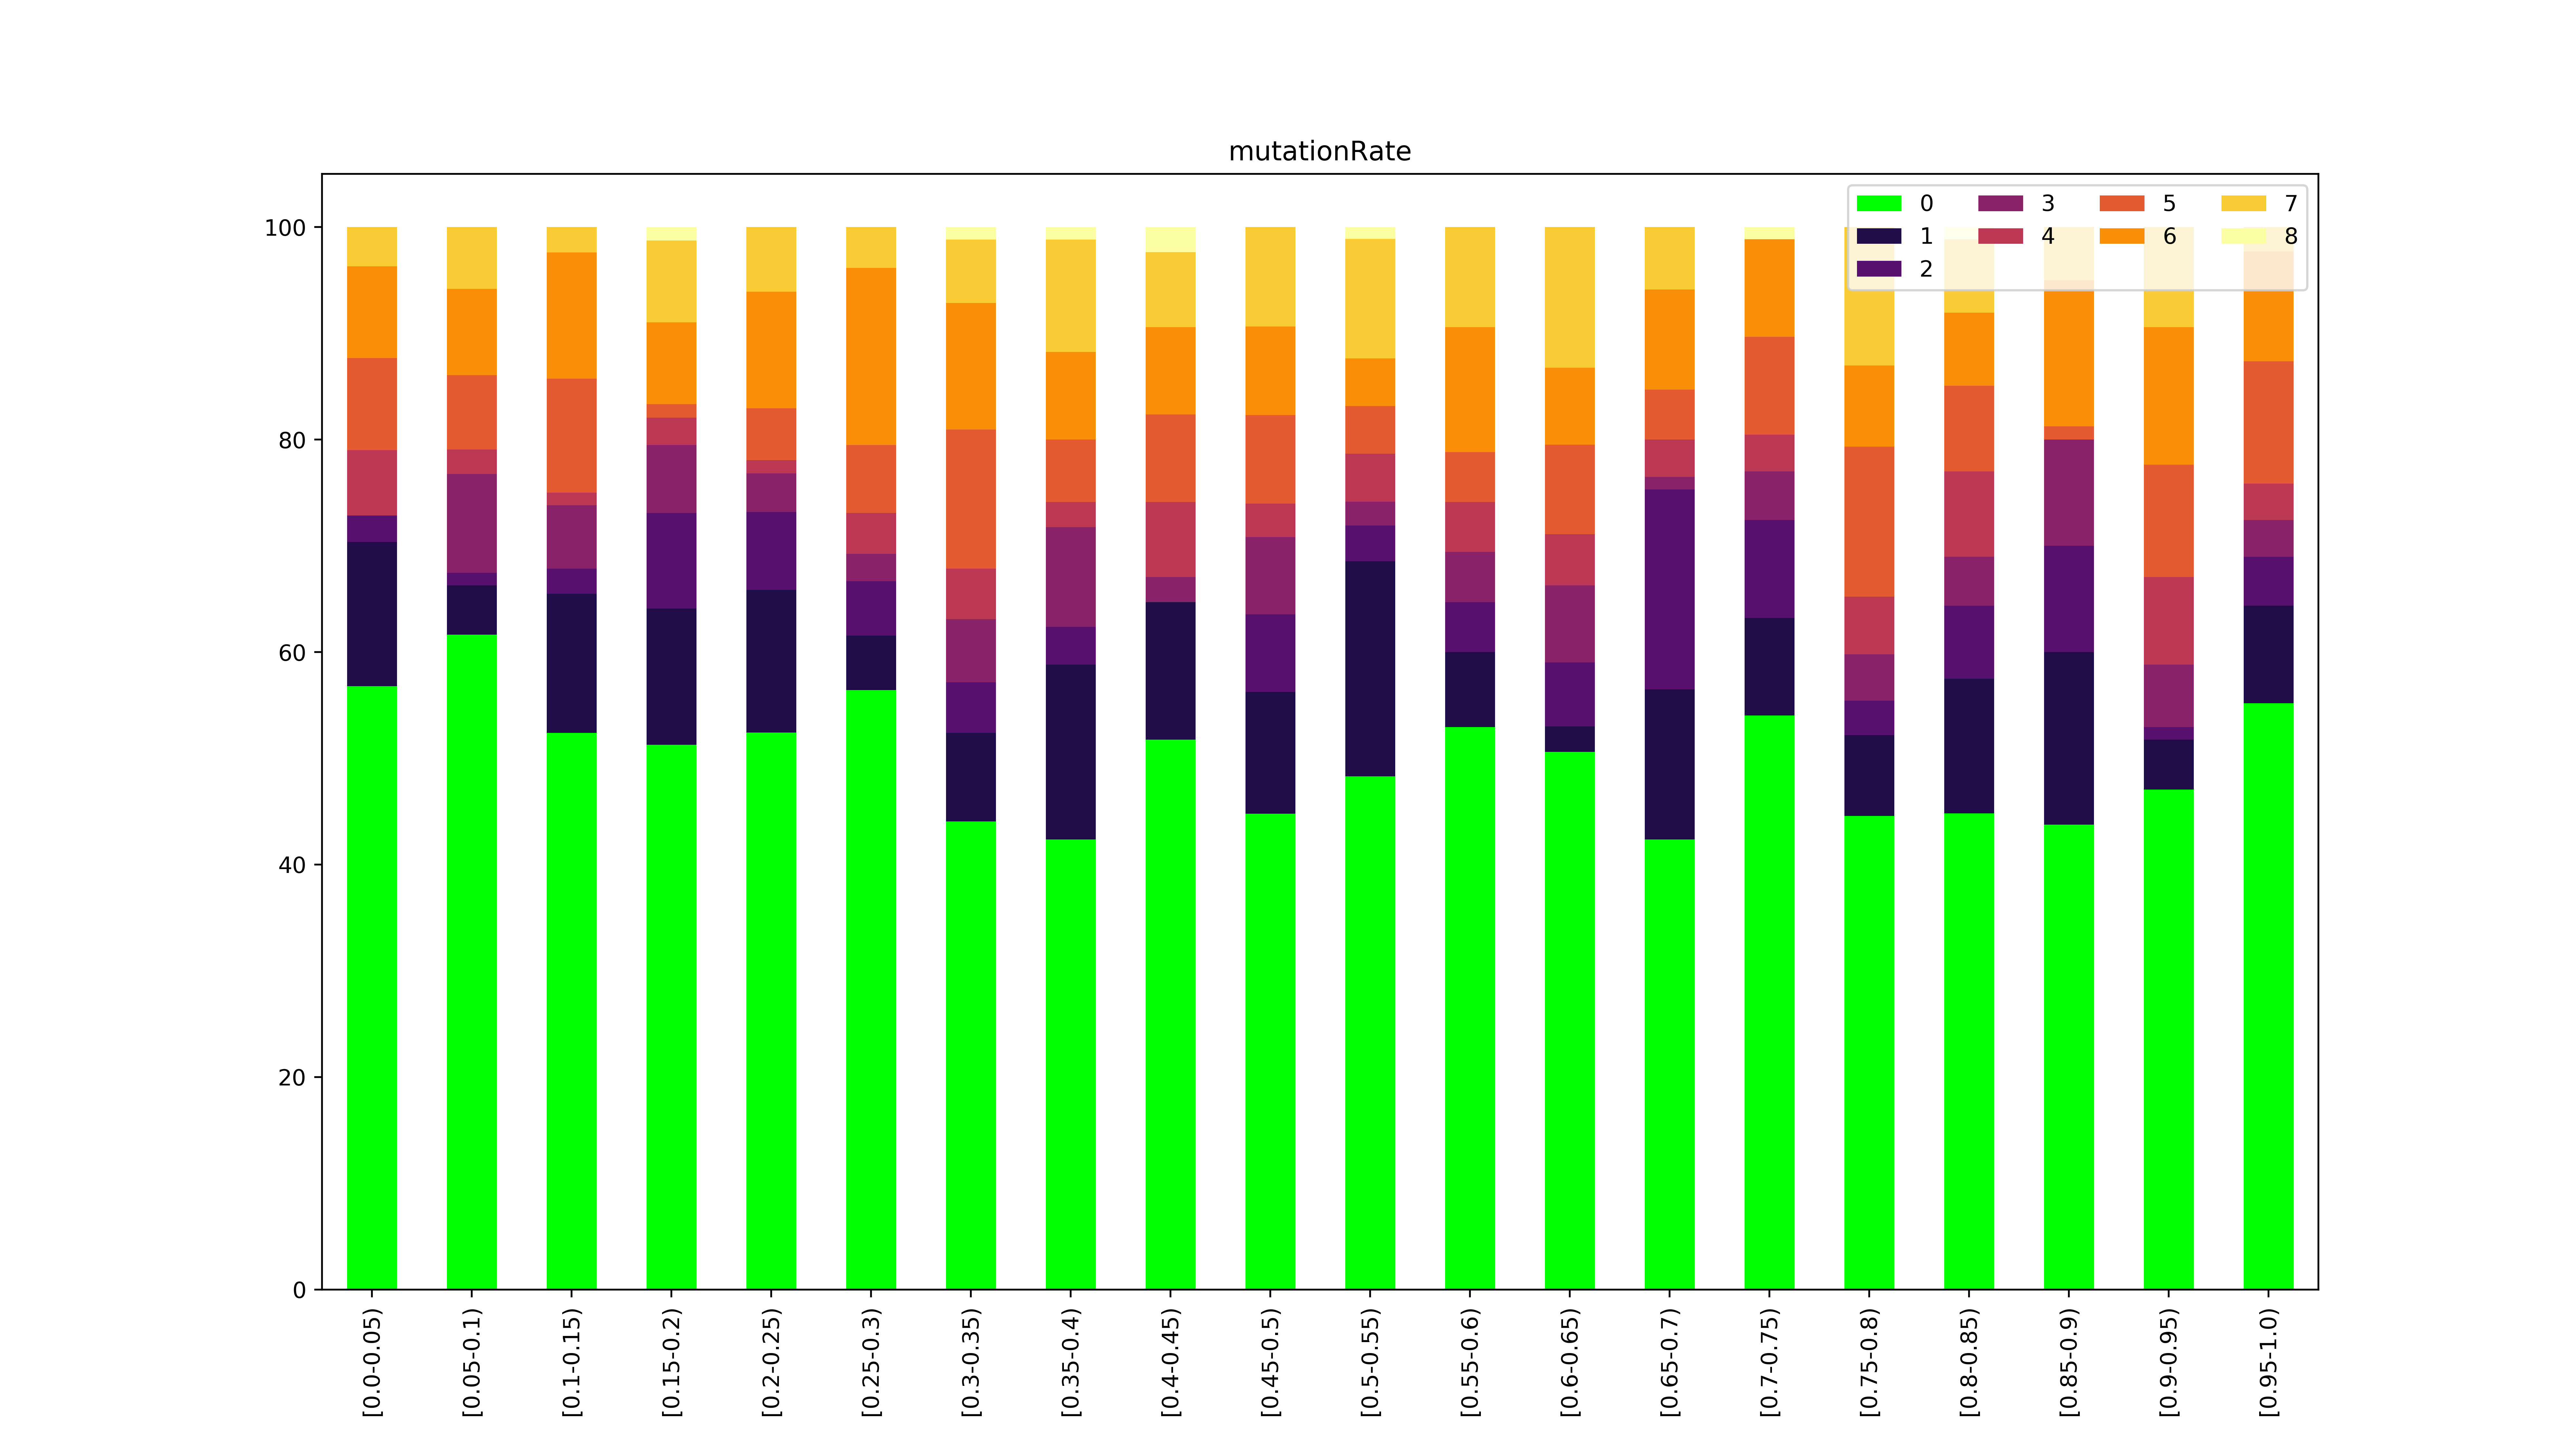
\includegraphics[width=\textwidth]{images/mutationRate_gradient_500dpi.png}
	\caption[]]{}
	\label{fig:mutationRate_gradient}
\end{figure}

The two types of distribution of parameter value and number of contract violation were discussed. Distributions for both problems for each parameter presented in Appendix\ref{label}. These plots confirm the conclusions that we made above. Values of some parameters such as \texttt{populationSize}~(R3), \texttt{crossoverRate}~(R5), \texttt{populateSoftwareSolutionAttempts}~(R13) and \texttt{crossoverOnRandomRequestProbability}~(R16) have a higher effect on the result.
The distribution  of the \texttt{crossoverOnRandomRequestProbability}~(R16) parameter showed in Appendix~\ref{label} confirms conclusions from correlation analysis that lower value gives better result. 
Some parameters give "good" and "bad" results for all values. That means that we could remove them from the parameter tuning and use constant value. Furthermore, for other parameters, values ranges could be adjusted.

To answer the question of what value of parameters with no obvious advantage in distribution, we construct a similar distribution with the quality of the solution.
As earlier we presented two distribution for \texttt{populationSize}~(R3) and \texttt{mutationRate}~(R7) parameters for smaller problem for smaller problem.

Figure~\ref{fig:populationSizeObjective} shows the quality distribution for the \texttt{populationSize}~(R3). This distribution differs from the previous one shown in Figure~\ref{fig:populationSize_gradientSmall} that all non-valid configurations are located in one segment that marked as "non-valid" and have a black color. Valid results consist of segments with different high and color. Each segment represents the percentage of the total number of configurations that have the same parameter value and which give the result near the same quality. All colors except black show the deviation of the quality of the solution from optimum in percent. Greed color represents optimal solutions.

As we can see, if a genetic solver gets valid results, the quality of the solution is optimal, or near-optimal. This distribution also confirms conclusions in Section~\ref{sec:evaluation}.

For current analysis the distribution of the \texttt{mutationRate}~(R7) parameter is more interesting and it showed in Figure~\ref{fig:mutationRateObjective}. The distribution of contract violations shows that any value of the parameter could give a valid result. However, the distribution of quality shows that some values of the parameter could give an optimal solution to the problem. Let us compare two ranges of values [0.45, 0.5) and [0.75, 0.8). Both ranges have near the same percentage of valid results of 50\%.
Nevertheless, the first range could give an optimal solution. The second range could not give such a solution. Moreover, the percentage of near-optimal solutions for the second range is lower.


\begin{figure}
	\centering
	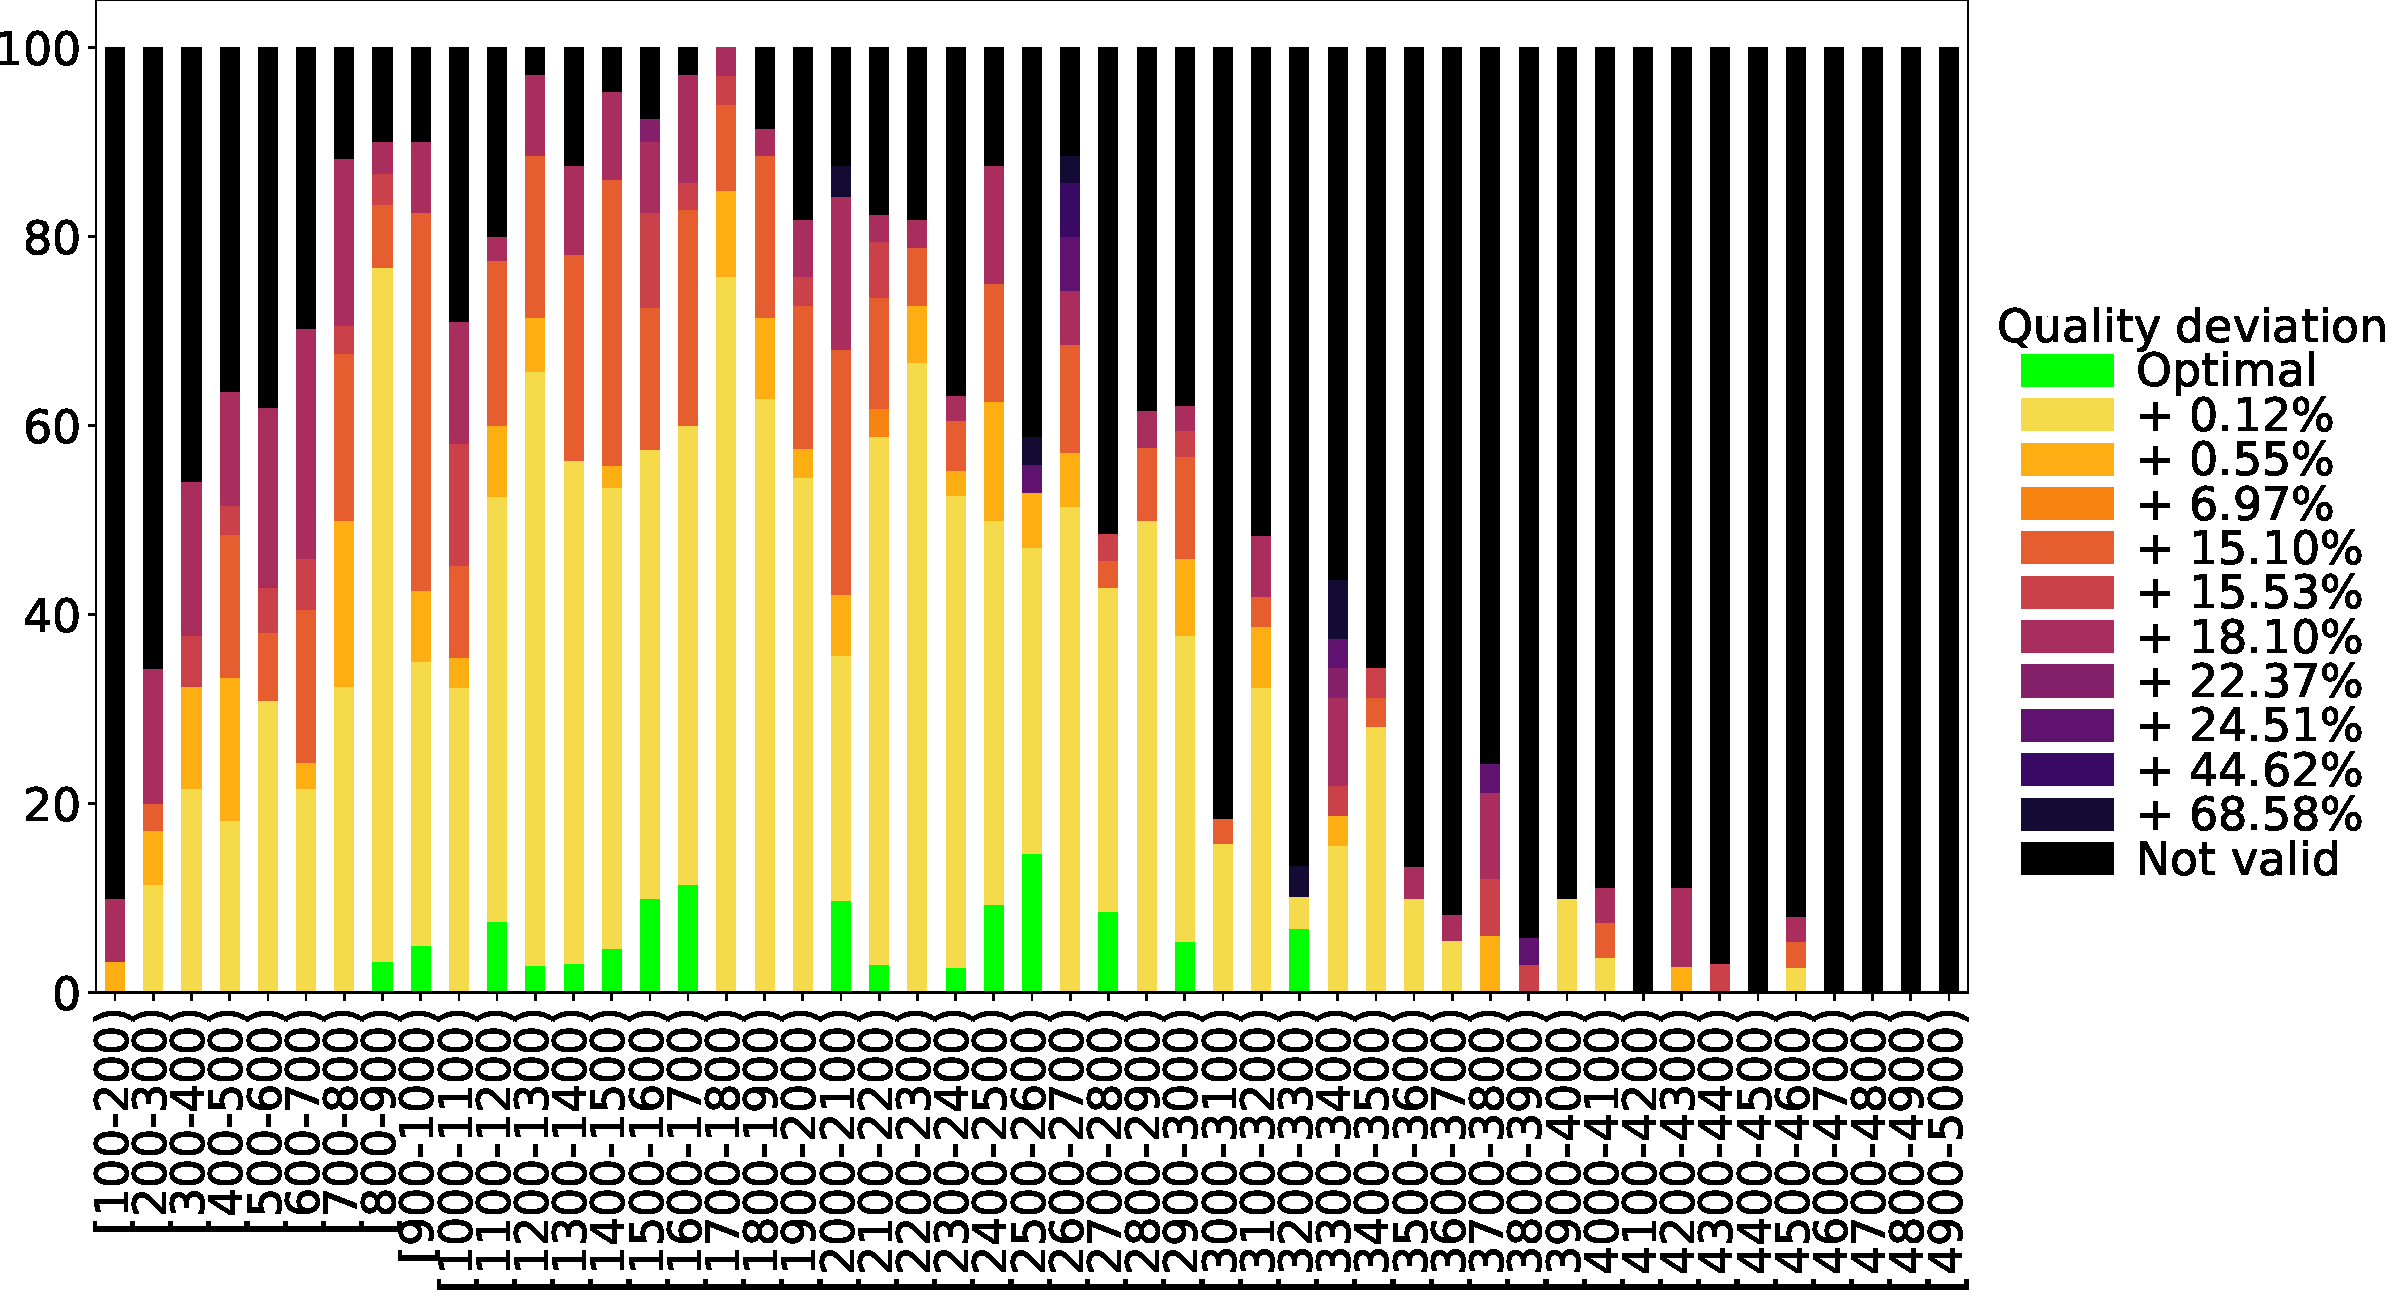
\includegraphics[width=\textwidth]{images/populationSizeObjective.pdf}
	\caption[]]{}
	\label{fig:populationSizeObjective}
\end{figure}


\begin{figure}
	\centering
	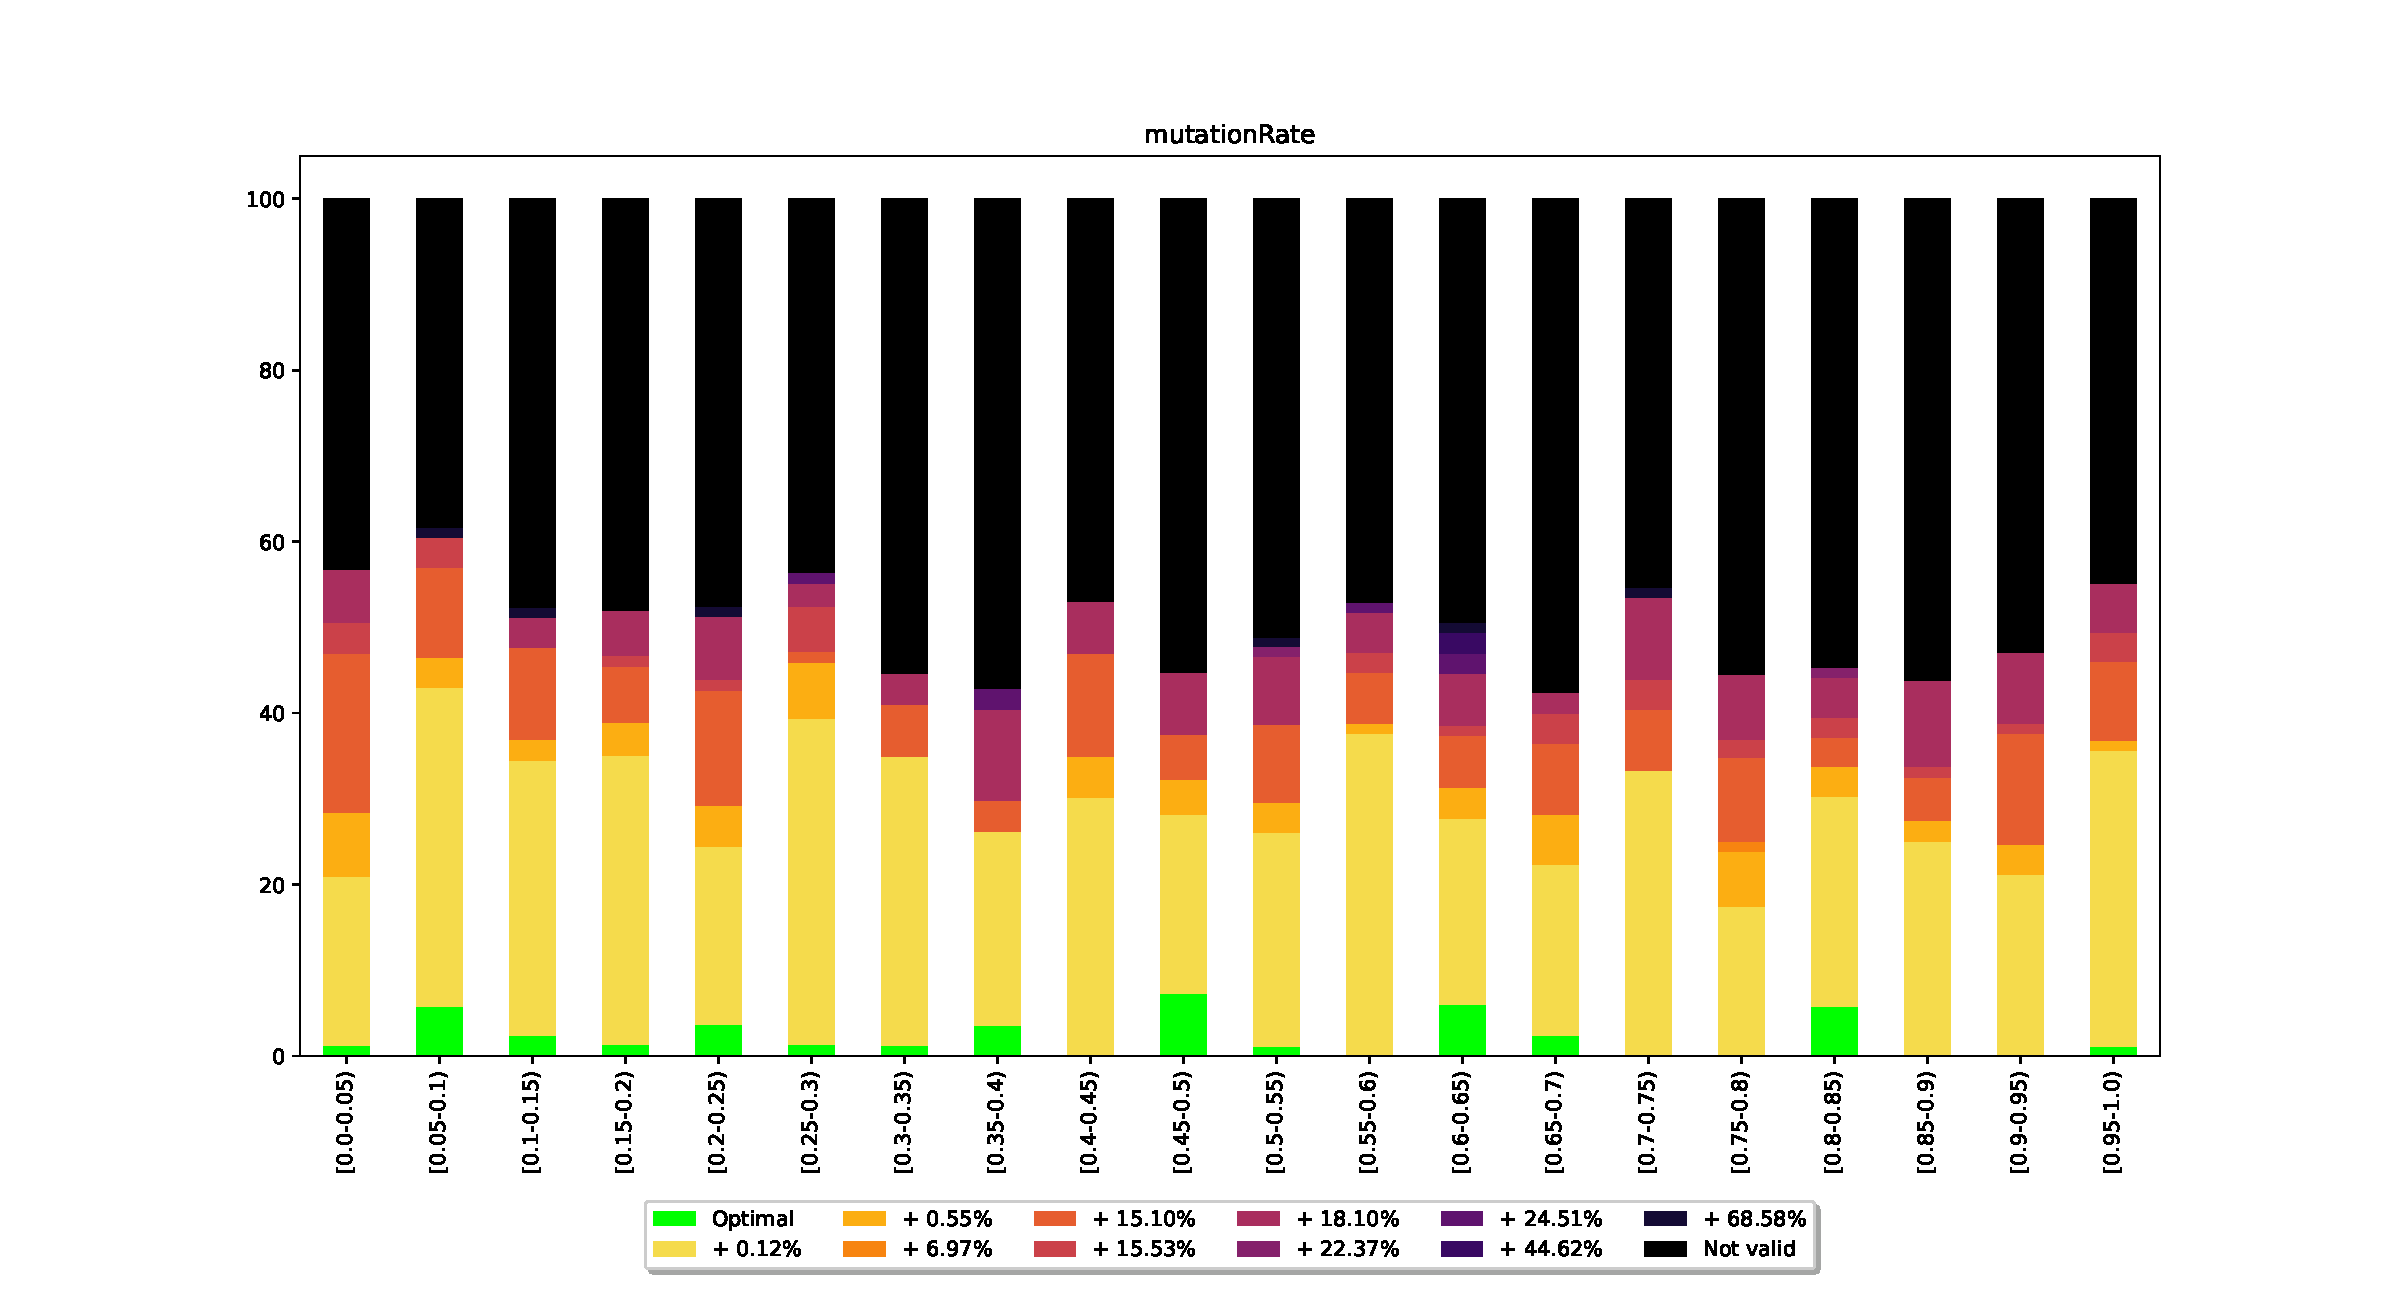
\includegraphics[width=\textwidth]{images/mutationRateObjective.pdf}
	\caption[]]{}
	\label{fig:mutationRateObjective}
\end{figure}

Last discussed plots shows that validity of the result that described as a number of contract violation could not depend on the value of the parameter. However, the quality of the solution depends on the parameter value. As a conclusion, we could say that we could remove some parameters from the parameter tuning if our goal is to find a valid solution. But if we are looking for the best quality of the solution, it needs all the parameters. This fact shows that multi-objective optimization is a complex question.
\chapter{Conclusion}
Parameter tuning works on genetic algorithms well, but not all tasks could be solved by GA.
\chapter{Future work}

The research presented in this thesis shows that the Parameter Tuning could improve the Genetic Solver. However, it is not enough to solve big sized Problems. As mentioned in Section\ref{sec:GeneticAlgorithm:Selector}, there is a framework limitation of used selector algorithms. There is a possibility that another selection algorithm for EA could further improve results. Because during the tuning parameter, BRISE gave optimized parameters that differed only in the selector.

Genetic solver without duplicates~(WD) is a possible starting point for the feature research. We show that this modification works slower than other approaches because it compares each new individual with a set of unique individuals in the population. Nevertheless, the WD and WD-T versions of the genetic solver give results with good quality in less number of generation. Better implementation of this approach could improve the results of the genetic solver.

Another starting point for the future work is a parameter control inside the genetic solver. It will change the parameters of the genetic solver on a fly. 

%\chapter{Einleitung}\label{ch:introduction}
Thematische Einführung, Motivation

\paragraph{Ziel der Arbeit:} Konzept entwickeln, welches Zonenbasierte MRI mit Kraftsteuerung vereinigt.

Aufbau der Thesis vorstellen

In~\Cref{ch:conclusion} kommt die Zusammenfassung.

%\chapter{Grundlagen}\label{ch:basics}

\section{Figures, Zitate, Mathe}
\begin{figure}[h]
\centering
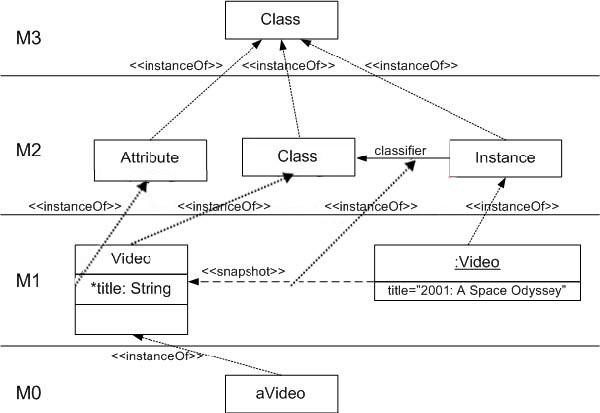
\includegraphics[scale=0.8]{OMG_MOF_4levels}
\caption{Das ist eine schlechte Grafik --- zu viele Pixel. Versuche Vektorgrafiken zu nutzen. Selbst malen geht gut mit draw.io powerpoint
  oder inkscape}\label{fig:mof}
\end{figure}

Wenn eine Abbildung verwendet wird, muss diese immer unbedingt im Text referenziert und beschrieben werden.
Z.B. so: \Cref{fig:mof}.

Zitieren geht so~\cite{haddadin2013towards}.

Math:

$A = \{x | x \in Y\}$

\begin{defs}\label{def:abc}
    A \textbf{Petrinet} is a tuple ${\Sigma = (P, T, F, W)}$.
\end{defs}

Petrinets are defined in~\Cref{def:abc}. See at the head of this document how to create your own definitions/lemma environments.


\subsection{Installation}
\textbf{Windows:} miktex

\textbf{Linux:} texlive-full

\textbf{GUI-Editor} texstudio

Konfiguration vom Editor: Preferences > Build
* default compiler: \emph{latexmk}


\section{Was ist ABC?}

\blindtext

%\chapter{Problemanalyse und Modellierung}

\blindtext
\todo[inline]{Write some more}

\begin{lstlisting}[language=AST,label={lst:example-ast},caption={Example AST}]
RailwayContainer ::= Route* Region*;
abstract RailwayElement ::= <Id:int>;
Region : RailwayElement ::= TrackElement* Sensor*;
Semaphore : RailwayElement ::= <Signal:Signal>;
Route : RailwayElement ::= <Active:boolean> SwitchPosition*;
SwitchPosition : RailwayElement ::= <Position:Position>;
Sensor : RailwayElement;
abstract TrackElement:RailwayElement;
Segment : TrackElement ::= <Length:int> Semaphore*;
Switch : TrackElement ::= <CurrentPosition:Position>;
\end{lstlisting}
%
Das Listing~\ref{lst:example-ast} zeigt eine beispielhafte Grammatik, welche im Attribute im folgenden Listing genutzt wird:

\lstinputlisting[language=JRAG,style=unboxed]{code/requiredSensor.jrag}

%\chapter{Erprobung der Anwendungsinstallation}\label{ch:evaluation}

\blindtext

%\chapter{Zusammenfassung}\label{ch:conclusion}

\blindtext


\printbibliography[heading=bibintoc]\label{sec:bibliography}

%\appendix
%\chapter{Weitere Latex-Dokumentation}
Nachdem nun der Vorspann und~-- bis auf das Literaturverzeichnis am
Ende des Dokumentes auf Seite~\pageref{sec:bibliography}~-- alle
Verzeichnisse erfolgreich ausgegeben wurden, wird nun die Verwendung
der weiteren Umgebungen und Befehle demonstriert, welche im Tutorial
\texturn{treatise.pdf} vorgestellt wurden.

\section{Referenzen und das Literaturverzeichnis}
Das Literaturverzeichnis wird auf Basis der nachfolgend verwendeten
Zitate erstellt und ist auf Seite~\pageref{sec:bibliography} zu finden.
In diesem Textabschnitt werden die zwei bekannten \LaTeX-Bücher
\cite{knuth84} und \cite{goossens94} sowie das Anwenderhandbuch
\cite{hanisch14} zitiert.p

\section{Grafiken und Tabellen in Gleitumgebungen}
Es folgt die Demonstration von Gleitumgebungen, welche sowohl für
Grafiken als auch Tabellen verwendet werden sollten. Im vorliegenden
Beispiel kann unter Umständen der Eindruck entstehen, dass diese Seite
etwas zu überladen mit Gleitobjekten ist. Dies liegt nicht an der
Verwendung der Gleitobjekte sondern vielmehr am zu geringen Textvolumen
und den eingeschränkten Möglichkeiten von \LaTeX{}, diese an geeigneten
Stellen zu platzieren.

\subsection{Abbildungen als Gleitobjekte und das Einbinden von Grafiken}
In \autoref{fig:example} wird dargestellt, wie eine Grafik im PDF"~Format
in ein Dokument eingebunden und auf diese verwiesen werden kann. Ein
Querverweis auf ein Gleitobjekt sollte im Fließtext am besten mit Befehl
\texttt{\textbackslash autoref\{\emph{<Label>}\}} erstellt werden.
Hierfür ist ein entsprechender Anker am zu referenzierenden Objekt nötig,
welcher mit dem Makro \texttt{\textbackslash label} erzeugt wird. Dabei
ist entscheidend, dass dieser Anker erst \emph{nach} der Beschriftung des
Objektes, welche mit \texttt{\textbackslash caption} zu erstellen ist,
definiert werden sollte.

\begin{figure}
\centering
\includegraphics{TUD-black}
\caption{Beispielgrafik}\label{fig:example}
\end{figure}

\subsection{Untergleitobjekte}
Nachdem nun schon eine gleitende Abbildung und zwei gleitende Tabellen
erstellt wurden, folgt jetzt noch eine gleitende Abbildung mit zwei
Unterabbildungen. Durch die drei gesetzten Anker kann im Fließtext
sowohl auf \autoref{fig:logos} als auch auf \autoref{fig:tud} sowie
\autoref{fig:ddc} verwiesen werden.

\begin{figure}
\ffigbox[\FBwidth]%
  {\begin{subfloatrow}%
    \ffigbox[\FBwidth]%
      {\fbox{\includegraphics[height=2cm]{TUD-black}}}%
      {\caption{Eine Abbildung}\label{fig:tud}}%
    \ffigbox[\FBwidth]%
      {\fbox{\includegraphics[height=2cm]{DDC-21}}}%
      {\caption{Eine weitere Abbildung}\label{fig:ddc}}%
  \end{subfloatrow}}%
  {\caption{Eine Gleitumgebung mit zwei Abbildungen}\label{fig:logos}}%
\end{figure}

\subsection{Tabellen als Gleitobjekte}
Tabellen sollten in der \texttt{table}"=Gleitumgebung gesetzt werden.
Welche Umgebung für die Tabelle selbst dabei genutzt wird ist dabei
nicht relevant. Es können sowohl die normale \texttt{tabular}"=Umgebung
als auch die Umgebungen \texttt{tabularx}, \texttt{tabulary} sowie
\texttt{tabu} für variable Spaltenbreiten bei einer fest vorgegebenen
Tabellenbreite oder jede andere Tabellenumgebung genutzt werden.
Nachfolgend wird dies an mehreren Beispielen demonstriert.

\subsubsection{Eine gleitende tabularx-Tabelle}
Es wird eine Tabelle mithilfe der \texttt{tabularx}"=Umgebung erstellt.
Zu sehen ist diese in \autoref{tab:tabularx}. Für diese werden zuvor
neue Spaltentypen definiert.

\newcolumntype{Y}{>{\hspace{0pt}}X}
\newcolumntype{D}{>{\raggedright}Y}
\newcolumntype{E}{>{\centering}Y}
\newcolumntype{F}{>{\raggedleft}Y}

\begin{table}
\begin{tabularx}{\textwidth}{@{}EEEEE@{}}
\toprule
\textbf{Problem ID} & \textbf{Basic} &
\textbf{with new probabilities} & \textbf{without duplicates in population} & \textbf{without duplicates in population + tuning} 
\tabularnewline
1 & 1.23 & 0.01 & 0 & 0
\tabularnewline
10 & 0.26 & 0.01 & 0 & 0
\tabularnewline
13 & 1.23 & 0.01 & 0 & 0
\tabularnewline
19 & 1.23 & 0.01 & 0 & 0
\tabularnewline
28 & 1.23 & 0.01 & 0 & 0
\tabularnewline
31 & 1.23 & 0.01 & 0 & 0
\tabularnewline
\bottomrule
\end{tabularx}
\caption{Eine \texttt{tabularx}"=Tabelle}\label{tab:tabularx}
\end{table}

\subsubsection{Eine gleitende tabulary-Tabelle}
Es wird eine Tabelle mithilfe der \texttt{tabulary}"=Umgebung erstellt.
Zu sehen ist diese in \autoref{tab:tabulary}.

\begin{table}
\begin{tabulary}{\textwidth}{@{}LCRJ@{}}
\toprule
\textbf{Linksbündig} & \textbf{Zentriert} &
\textbf{Rechtsbündig} & \textbf{Blocksatz} \tabularnewline\midrule
Ein linksbündiger Blindtext zur Demonstration einer L"~Spalte &
Ein zentrierter Blindtext zur Demonstration einer C"~Spalte &
Ein rechtsbündiger Blindtext zur Demonstration einer R"~Spalte &
Ein wesentlich längerer und absolut inhaltsleerer Blindtext im
Blocksatz für eine um einiges bessere Demonstration einer J"~Spalte
\tabularnewline\bottomrule
\end{tabulary}
\caption{Eine \texttt{tabulary}"=Tabelle}\label{tab:tabulary}
\end{table}

\subsubsection{Eine gleitende tabu-Tabelle}
In \autoref{tab:tabu} ist eine weitere Tabelle mit variabler Breite der
Spalten und festgelegter Gesamtbreite zu sehen, welche in der Umgebung
\texttt{tabu} gesetzt wurde. Auch für diese wird zuerst ein neuer
Spaltentyp definiert, der die Unzulänglichkeiten der Umgebung reduziert.
Mit \texttt{\textbackslash ttabbox} aus dem Paket \texttt{floatrow} wird
die Beschriftung auf die Breite der Tabelle begrenzt.

\makeatletter
\newcolumntype{Z}{}
\renewcommand*{\NC@rewrite@Z}[1][]{%
  \NC@find>{\hspace{0pt}}X[#1]<{\@finalstrut\@arstrutbox}%
}
\makeatother

\begin{table}
\ttabbox{%
  \begin{tabu} to .8\textwidth {@{}Z[3,l]Z[3,c]Z[3,r]Z[2,j]@{}}
    \toprule
    \textbf{Linksbündig} & \textbf{Zentriert} &
    \textbf{Rechtsbündig} & \textbf{Blocksatz} \tabularnewline\midrule
    Ein linksbündiger Blindtext zur Demonstration einer Z[l]"~Spalte &
    Ein zentrierter Blindtext zur Demonstration einer Z[c]"~Spalte &
    Ein rechtsbündiger Blindtext zur Demonstration einer Z[r]"~Spalte &
    Ein Blindtext im Blocksatz innerhalb einer Z"~Spalte
    \tabularnewline\bottomrule
  \end{tabu}%
}{%
  \caption[Eine \texttt{tabu}"=Tabelle]{%
    Eine \texttt{tabu}"=Tabelle in Verbindung mit dem Befehl
    \texttt{\textbackslash ttabbox}, welcher vom Paket \texttt{floatrow}
    für Beschriftungen in Objektbreite bereitgestellt wird%
  }%
  \label{tab:tabu}%
}
\end{table}

\section{Zitate}
Bei der Verwendung von wörtlichen Zitaten sollten diese als solche
gekennzeichnet werden.
\enquote{Dies ist ein zugegebenermaßen nicht sehr sinnvolles Zitat.}
\cite[58]{hanisch14}
Für eine möglichst gut nachvollziehbare Referenz sollte nicht nur
das Werk selber sondern zumindest die Seitenzahl und gegebenenfalls
der Absatz der originalen Textstelle angegeben werden.
\begin{quoting}
\enquote{%
  Dies ist ein noch sinnloseres Zitat. Allerdings wird zumindest die
  Wirkung der Umgebung \texttt{quoting} bei der Absatzauszeichnung
  deutlich.

  Wie zu sehen ist, wird der zweite Absatz~-- wie jeder weitere~--
  aufgrund der Option \texttt{parskip=false} eingezogen.
}
\cite[sinngemäß nach][\pno{} 12, zweiter Absatz]{hanisch14}
\end{quoting}
Ebenfalls sollten sinngemäße Zitate mit einer möglichst genauen Referenz
angegeben werden. Dies kann im Laufe der Arbeit auch für einen selbst von
Vorteil sein, wenn beispielsweise die originale Textpassage noch einmal
analysiert werden soll.


\confirmation

\end{document}
